%% DO NOT FORGET PART
% THE JUSTIFICATIONS IN THE EXPERIMENTAL PART FOR THE LOADED AND NO-LOAD CONDITIONS ARE NOT GOOD
% DOING THE SIMULATIONS RELATED TO FIG 16 TO MAKE IT FOR 2 AMP OF REFERENCE POINT
% DEFINING I_REF AND INTRODUCING ITS NUMBER FOR FIG 16 AND SOMEHWERE IN THE EXPERIMENTAL RESULTS
% PARAGRAPH "HAVE A LOOK AT ME"
% TEMPLATE
\documentclass[journal,a4paper,10pt,twoside]{IEEEtran} % FOR THE FINAL REVISION
%\documentclass[journal,a4paper,10pt,twoside, peer review]{IEEEtran} %https://www.overleaf.com/project/5e2c41154c5dc6000173e05b FOR THE PEER REVIEW REVISION
% TEST2 (MADE ON DESKTOP)
% PACKAGES
\usepackage{import}
\usepackage{graphicx}
\usepackage{xcolor}
\usepackage{soul}
\usepackage{times}
\usepackage{epsfig}
\usepackage{amsfonts}
\usepackage{amssymb}
\usepackage{colortbl}
\usepackage{upgreek}
\usepackage{booktabs}
\usepackage{multicol}
\usepackage{lipsum}
\usepackage{cite}
\usepackage{amsmath}
\usepackage[cmintegrals]{newtxmath}
\usepackage{bm}
\usepackage{url}
\usepackage{subfig}
\usepackage{multirow}
\usepackage{array}
\usepackage{dblfloatfix}
%\usepackage{stfloats}  %% PLEASE DO NOT USE THIS, INSTEAD, USE DBLFLOATFIX!
\usepackage{dblfloatfix}
\usepackage{adjustbox}

\usepackage{kantlipsum} % EXAMPLE FOR AN ENGLISH ARTICLE

% STRUCTURE

\hyphenation{op-tical net-works semi-conduc-tor}

\begin{document}
	
	%\title{DPM for Suppression of Mode-Changing Transients in WPT Transmitters}	%STARTS THE TITLE AND TITLE AREA
	%\title{SPI Controller for LCC Networks used in WPT Applications}
	%\title{SPI Controller to Stabilize LCC Networks used in WPT Applications}
	\title{{\color{blue}Single-Oriented} PWM-Synchronized Sampling Technique for Stabilizing LCC Networks used in WPT Applications}
	
	\author{\IEEEauthorblockN{
        Farzad Farajizadeh,~\IEEEmembership{Member,~IEEE,}
        D. Mahinda Vilathgamuwa,~\IEEEmembership{Fellow,~IEEE,}
        Dejan P. Jovanovic,~\IEEEmembership{Member,~IEEE,}
        and Gerard Ledwich,~\IEEEmembership{Fellow,~IEEE}}
        
		\thanks{
			F. Farajizadeh, D. M. Vilathgamuwa, D. P. Jovanovic, and G. Ledwich are with the Department of Electrical Engineering and Computer Science, Queensland University of Technology, Brisbane, QLD 4001, Australia (e-mail: f.faradjizadeh@gmail.com; mahinda.vilathgamuwa@qut.edu.au; g.ledwich@qut.edu.au).
		}
	}
	
	%\markboth{Journal of \LaTeX\ Class Files,~Vol.~14, No.~8, August~2015}
	%{Shell \MakeLowercase{\textit{et al.}}: Bare Demo of IEEEtran.cls for IEEE Journals}
	
	
	%\IEEEpubid{\begin{minipage}{\textwidth}\ \\[12pt] \centering
	%	1551-3203 \copyright 2015 IEEE. Personal use is permitted, but republication/redistribution requires IEEE permission.\\
	%	See http://www.ieee.org/publications standards/publications/rights/index.html for more information.
	%	\end{minipage}}
	
	%\IEEEspecialpapernotice{(Invited Paper)}	
	%\IEEEpubidadjcol 							% PLEASE, DO NOT FORGET TO USE ME AT THE END OF EACH PAGE TO MAKE YOUR COLUMNS NEAT. I AM ALSO USEFUL FOR ID NUMBER NOT TO BE OVERFLOWN.
	
	
	\maketitle % ENDS THE TITLE AREA
	
	\begin{abstract}
		This paper presents a new method of {\color{blue}Single-Oriented} PWM-Synchronized Sampling (SOPWMS2) to estimate the envelope of a high frequency Alternating Current (AC) signal obtained from a {\color{blue}high order system}.
		Synchronized by the PWM signal of the supplying converter, features such as the envelope estimated at a minimum rate of sampling, and the absence of extra low-pass filters in reconstructing the envelope signal make this technique significantly simple to be implemented in high frequency applications, such as Wireless Power Transfer (WPT) systems. To demonstrate how SOPWMS2 operates, a new concept of vertically shifted transfer function is proposed and used to model the plant around its steady state frequency of operation. The obtained asymmetric transfer function can represent the envelope of the output signal when it is fed by the envelope of the input signal. {\color{red}Having the dominant orientation of the obtained envelope transfer function in the concerned operational bandwidth (frequency domain), the sampling instance with reference to the power converter PWM signals is determined, and the controller can be tuned accordingly.} To study the operation of the proposed technique, an LCC compensated wireless power transmitter is considered as a high order plant, then with the use of SOPWMS2 technique and a PI controller, a simple feed-back loop is closed to stabilize and control the transmitter current. Finally, the system is numerically simulated and experimentally tested, and the results verify the proposed approach.
	\end{abstract}
	
	\begin{IEEEkeywords}
        Current Control, Envelope Detection, LCC Compensator, Mode Changing Transients, Resonant Converter, Synchronized Sampling, Wireless Power Transfer (WPT).
    \end{IEEEkeywords}
	
	\ifCLASSOPTIONpeerreview
	\begin{center} \bfseries EDICS Category: 3-BBND \end{center}		% EXTRA INFORMATION ON THE COVER PAGE
	\fi
	\IEEEpeerreviewmaketitle											% INSERTS A PAGE BREAK AND MAKES THE SECOND TITLE
	
	\section{Introduction}
	
	\IEEEPARstart{H}{igh} frequency power transmission has been receiving increased attention with the growing demand for high power density electric devices. Increase of the operational frequency can reduce the size of electric devices, enhance their efficiencies, and pave the way for future utilization of special applications, namely wireless power transfer (WPT) systems.
	
	Unlike low and medium frequency applications, reconstructing the oscillating sampled signals in a discrete domain with conventional approaches is not easily achievable for high frequency systems. The main barriers of digital sampling in high frequency applications are the limits in the sampling rate and the delays resulted by data conversion and signal reconstruction \cite{fadali2013digital}.
	
	According to the Nyquist sampling theorem, to completely reconstruct an analogue oscillating signal in a discrete domain, the rate of sampling needs to be at least twice the frequency of oscillation \cite{NYQUIST_1,NYQUIST_2,NYQUIST_3}. Digital samplers are mostly carried out with the use of Zero-Order Hold (ZOH) technique, in which the sampler takes and holds the sampled data until the next sampling event \cite{fadali2013digital,ZOH}. This technique behaves as a low-pass filter and the decrease in the sampling frequency leads to the increased delay between the reconstructed digital signal and the input analog signal \cite{fadali2013digital}. {\color{blue}ZOH also mirrors the frequency content of the sampled data along a frequency which is half the sampling frequency.} Therefore, the sampling frequency needs to be properly selected to capture the desirable information from the input signal \cite{NYQUIST_2,NYQUIST_3,NYQUIST_4}. To appropriately reconstruct the sampled data, some low-pass filters can also be used. One of the well-known types of these low-pass filters is anti-aliasing, which prevents the frequency content around the Nyquist freqeuncy to influence the sampled data \cite{NYQUIST_4,NYQUIST_5,NYQUIST_6}. ZOH can also lead to some stability issues due to the unstable zeros in the discrete domain of the sampled system, which is exclusively studied by {\AA}str{\"o}m and Moore \cite{UNSTABLE_1,UNSTABLE_2}.
	
	Fortunately, in most of the high frequency applications, stabilizing and controlling the sub-harmonic dynamics of a high frequency AC signal are of the main goals, and the other harmonics are usually mitigated by the natural behavior of the system and additional filters and compensators, such as LCC and series capacitor compensators in WPT applications. This means sampling rate can be smaller than the Nyquist sampling rate corresponding to the signal fundamental frequency. {\color{blue}However, sub-harmonic dynamics of the signal is not directly achievable.}
	
	One of the most convenient ways to observe the sub-harmonic behavior of high frequency output signals is through their envelope \cite{ENVELOPE_1,ENVELOPE_2,ENVELOPE_3,ENVELOPE_4,ENVELOPE_5}. To extract the envelope of an AC signal, different approaches are presented and successfully used in industry, and some of them are briefly explained in the following.
	
	In extracting the envelope of an oscillating signal, {d-q} technique can be considered as one of the most reputed approaches. This method is based on Park transformation, and by determining the fundamental frequency of the oscillating signal, it can map the output(s) of the system on orthogonal direct (d) and quadrature (q) axes \cite{DQ_1,DQ_2,DQ_3} and reflect the fundamental frequency content of the signal as Direct Current (DC) values on the rotating {d} and {q} axes. 
	%% >> Literature Review
	Although this technique is extensively used in different applications, the need for knowing the fundamental frequency, the time delay produced by phase locked loop (PLL) controller to track the fundamental frequency, calculations needed for obtaining the envelope of the analogue signal (${\mathrm{r=\sqrt{d^2+q^2}}}$), and the presence of the undesirable double fundamental frequency content (and maybe other harmonics and sub-harmonics) in the obtained {d-q} signals make it a sophisticated choice for envelope detection at high frequencies.
	
	The other approach of envelope estimation is signal rectification. In this technique, the oscillating signal under study can be halved or fully rectified. The rectification is normally done with the use of active components, such as Op-Amps. Then the obtained rectified signal is fed to a low-pass filter to cancel out the second order harmonics \cite{REC_1,REC_2,REC_3,REC_4}. Simplicity of the structure makes this technique as an attractive option to be used in different applications.
	%% >> Literature Review
	Nevertheless, additive sub-harmonic noises, on the one hand, can produce an oscillating offset to the sampled signal, and consequently, increase the second order harmonic content the estimated envelope \cite{REC_4, REC_5}. On the other hand, the need for a low-pass filter can introduce a delay to the reconstructed envelope signal \cite{REC_1}.
	
	Therefore, in this article, taking the advantages of both {d-q} and signal rectification techniques, a new sampling technique is proposed that is able to effectively estimate the envelope of a high frequency oscillating signal. The simplicity of structure and low sampling rate make this technique suitable for high frequency applications. %{\color{red}However, the simplicity of structure is achieved at the cost of knowing the frequency response of the plant.}
	
	To illustrate this technique, a high frequency WPT system consisting of an LCC equipped transmitter and a series capacitor compensated receiver is considered as a case study. Although the provided principles are applicable for other types of systems, attractive features of LCC compensators in WPT applications, specially in dynamic chargers, make it an interesting high frequency system to be studied in this article \cite{farajizadeh, pantic, MPLCC}. The objectives considered for this system are to extract the envelope signal with the use of the proposed technique and fed it to a simple PI controller to stabilize the mode changing transients of the transmitter current.
	Mode changing transients in WPT systems, especially for dynamic chargers is a usual phenomenon \cite{farajizadeh,MODE_1,MODE_2,MODE_3}. This is mainly due to the frequent activation and deactivation of the transmitter pads depending on the receiver (pickup) position, as shown in Fig.~\ref{FIG1}. Selective excitation of the transmitter pads can decrease the power losses and improves the efficiency of the system \cite{farajizadeh,MODE_2,MODE_3}. Consequently, this can result in some harmful transients in the system that can influence the life-time and reliability of WPT systems.
	
	%%FIG1
	\begin{figure}
	    \centering
	    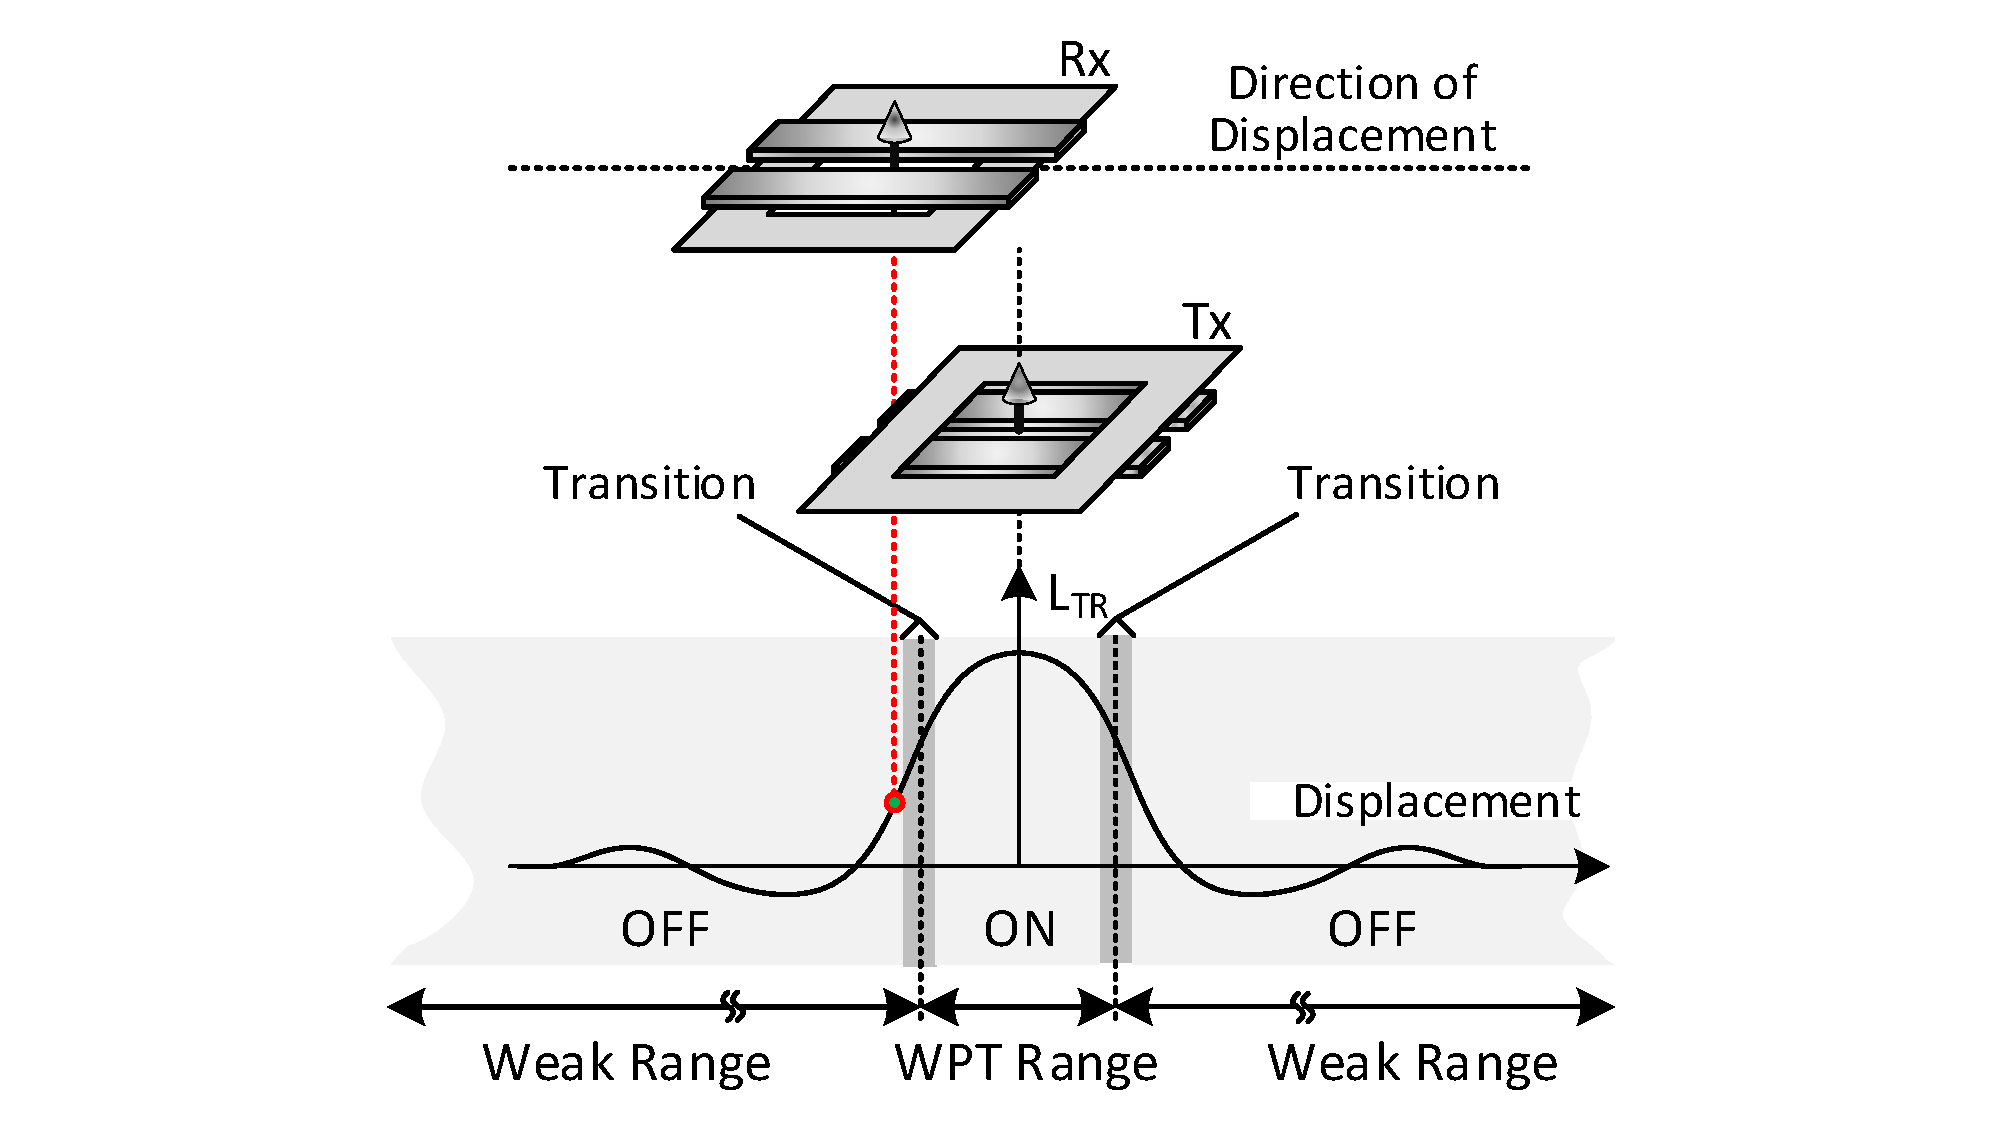
\includegraphics[clip, trim=2cm 0.5cm 2cm 0cm, width=0.8\columnwidth]{FIGS/FIG1.pdf}
	    \caption{Switching between different modes of operation in a transmitter pad with respect to the receiver position.}
	    \label{FIG1}
	\end{figure}
	
	To elaborate the proposed technique, the layout of this article is organized as follows. The WPT system under study is simplified as explained in Section II. Then the asymmetric transfer function of the envelope is obtained with a new concept of vertically shifted model, which is explained in section III. After determining the dominant behavior of the envelope transfer function, the new technique of sampling entitled as ``{Single-Oriented PWM-Synchronized Sampling} (SOPWMS2)" is proposed in Section IV. This section is also dedicated to the stability analysis of the system and tuning the controller. Finally, in Section V, the proposed technique is implemented in an experimental setup and the results are used to validate the proposed approach.

	\section{Detailed Model of the System}
	
	Dynamic response of a system is mostly influenced by the dominant natural frequencies (eigenvalues) that are closer to the fundamental frequency of operation and vertical axis $\mathrm{j}\omega$. {\color{blue}In this article}, the dynamic behavior of a WPT system shown in Fig.~\ref{FIG1} is to be studied. To this end, forming the state-space matrix equation is the starting point. This equation for the given system, neglecting the equivalent series resistors (ESRs) of the front-end inductor ($R_\mathrm{S}$) and the transmitter coil ($R_\mathrm{T}$), can be given as in \eqref{EQ1}.
	
	%%FIG2
	\begin{figure}
	%\vspace{-2mm}
	    \centering
	    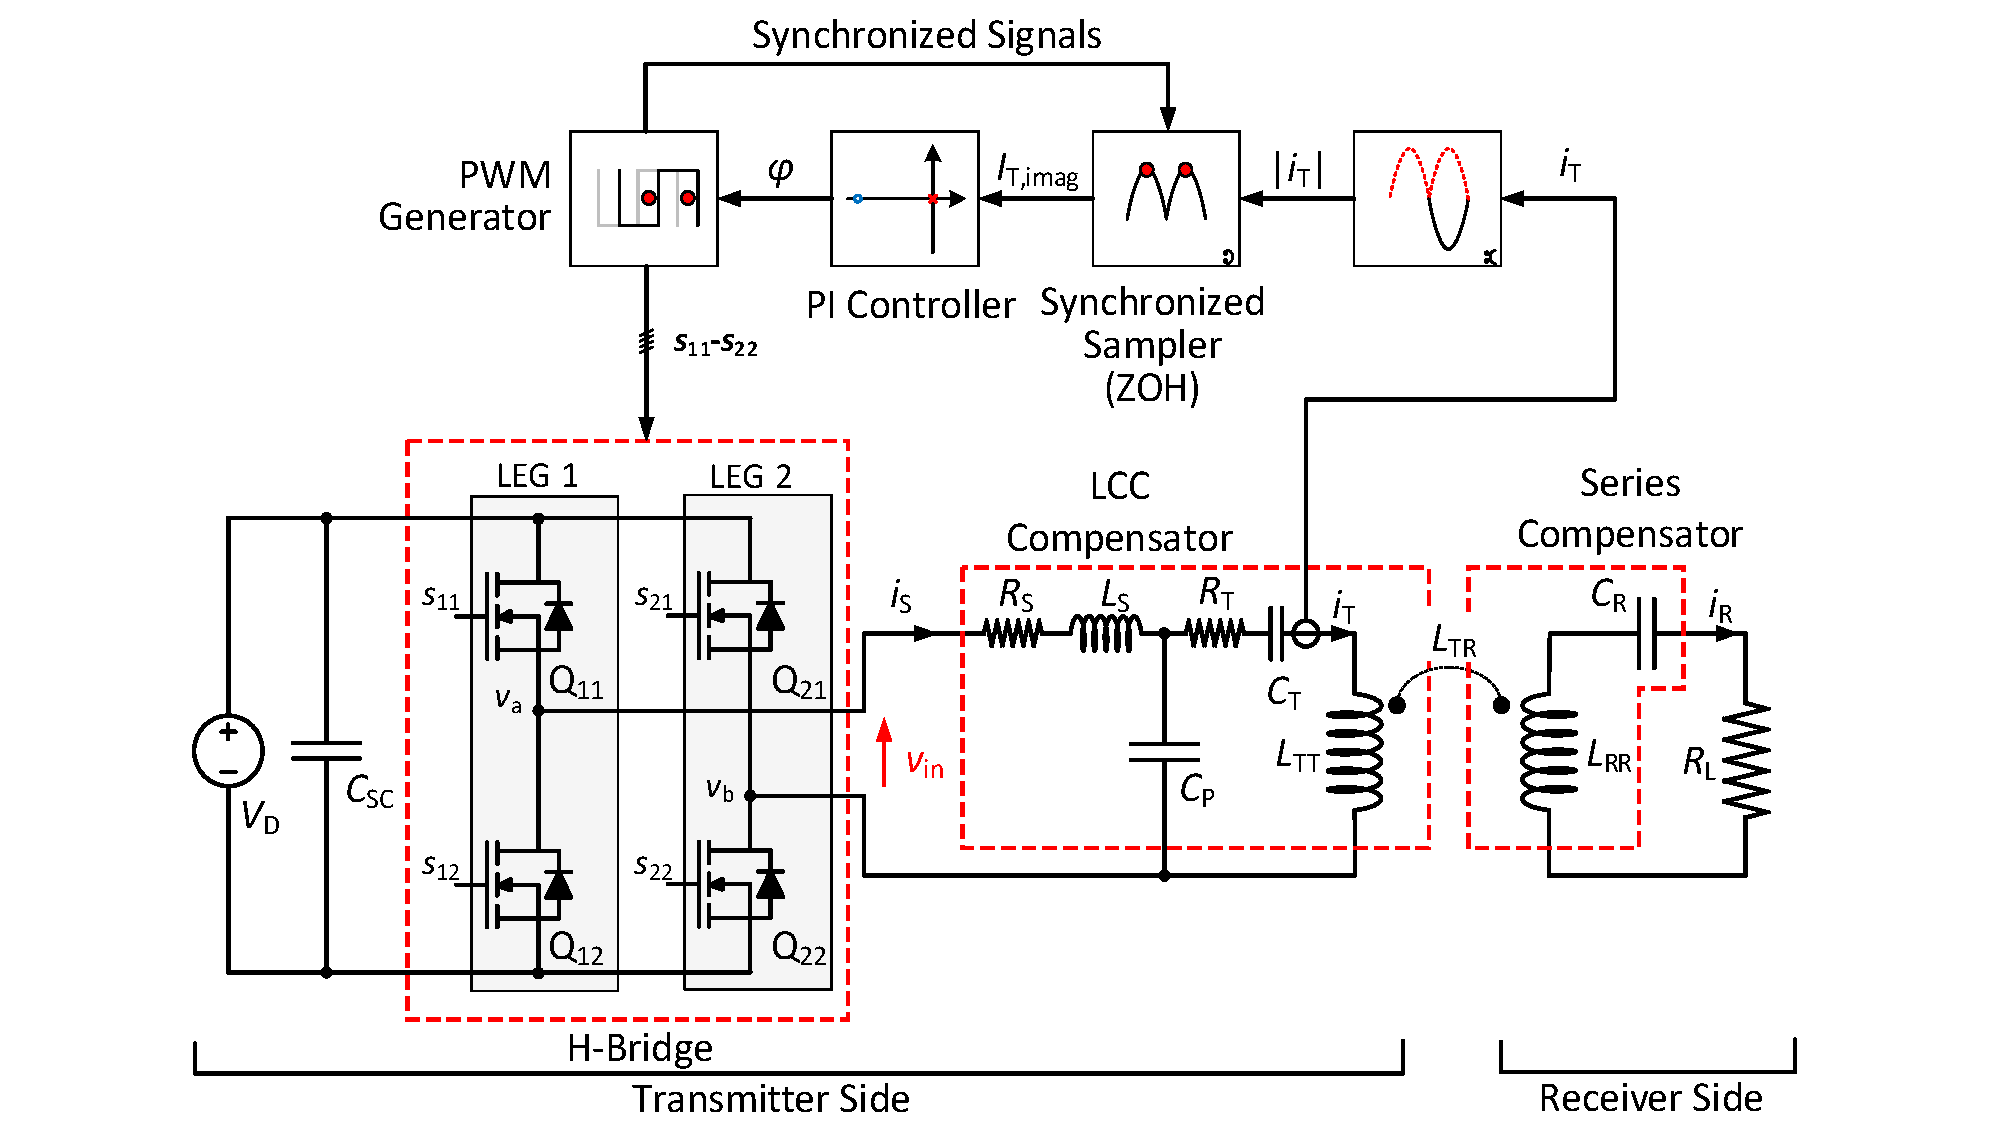
\includegraphics[clip, trim=3cm 0.25cm 3cm 0.25cm, width=1\columnwidth]{FIGS/FIG2.pdf}
	    \vspace{-5mm}
	    \caption{The WPT system compensated by an LCC compensator at the transmitter side and a series capacitor at the receiver side.}
	    \label{FIG2}
	    \vspace{-3mm}
	\end{figure}
	
	%%EQ1
	\begingroup
	\scriptsize
	%\vspace{-10mm}
	\begin{flalign}
	    s
	    %\times
	    \underbrace{
	    \begin{bmatrix}
	     {V}_\mathrm{P}\\{V}_\mathrm{T}\\{V}_\mathrm{R}\\{I}_\mathrm{S}\\{I}_\mathrm{T}\\{I}_\mathrm{R}
	    \end{bmatrix}
	    }_\textbf{X}
	    =
	    \underbrace{
	    \begin{bmatrix}
	        0                       &   0   &   0   &   \frac{1}{C_\mathrm{P}}   &   -\frac{1}{C_\mathrm{P}}  &   0\\
	        0                       &   0   &   0   &   0               &   \frac{1}{C_\mathrm{T}}   &   0\\
	        0                       &   0   &   0   &   0               &   0               &   \frac{1}{C_\mathrm{R}}\\
	        -\frac{1}{L_\mathrm{S}}          &   0   &   0   &   0               &   0               &   0\\
	        -\frac{L_{\mathrm{RR}}}{\Delta}  &   \frac{L_{\mathrm{RR}}}{\Delta} &   \frac{L_{\mathrm{TR}}}{\Delta}   &   0               &   0               &   \frac{R_\mathrm{L}L_{\mathrm{TR}}}{\Delta}\\
	        -\frac{L_{\mathrm{TR}}}{\Delta}  &   \frac{L_{\mathrm{TR}}}{\Delta} &   \frac{L_{\mathrm{TT}}}{\Delta}   &   0               &   0               &   \frac{R_{\mathrm{LL}}_{\mathrm{TT}}}{\Delta}
	    \end{bmatrix}
	    }_\textbf{A}
	    %\times
	    \underbrace{
	    \begin{bmatrix}
	     {V}_\mathrm{P}\\{V}_\mathrm{T}\\{V}_\mathrm{R}\\{I}_\mathrm{S}\\{I}_\mathrm{T}\\{I}_\mathrm{R}
	    \end{bmatrix}
	    }_\textbf{X}
	    +
	    \underbrace{
	    \begin{bmatrix}
	     0\\0\\0\\ \frac{1}{L_\mathrm{S}}\\0\\0   
	    \end{bmatrix}
	    }_\textbf{B}
	    %\times
	    \underbrace{
	    {V}_{\mathrm{in}}
	    }_\textbf{U} &&
	    \label{EQ1}
	    %\nonumber
	\end{flalign}
	\endgroup
	

	\noindent where \textbf{X} contains the state variables, which are the voltage across the parallel capacitor $C_\mathrm{P}$ (${V}_\mathrm{P}$), voltage across the transmitter series capacitor $C_\mathrm{T}$ (${V}_\mathrm{T}$), voltage across the receiver series capacitor $C_\mathrm{R}$ (${V}_\mathrm{R}$), current of the LCC front-end inductor $L_\mathrm{S}$ (${I}_\mathrm{S}$), current of the transmitter coil (${I}_\mathrm{T}$), and current of the receiver coil (${I}_\mathrm{R}$). Along with the self-inductance of the transmitter ($L_{\mathrm{TT}}$) and receiver ($L_{\mathrm{RR}}$), all the parameters in the state-matrix (\textbf{A}) are shown in Fig.~\ref{FIG2}. In this matrix, $\Delta$ is used for clarity, and it is equal to $L_{\mathrm{TR}}^2-L_{\mathrm{RR}}L_{\mathrm{TT}}$. 
	
	%%FIG3
	\begin{figure}
	\vspace{0mm}
	    \begin{center}
	            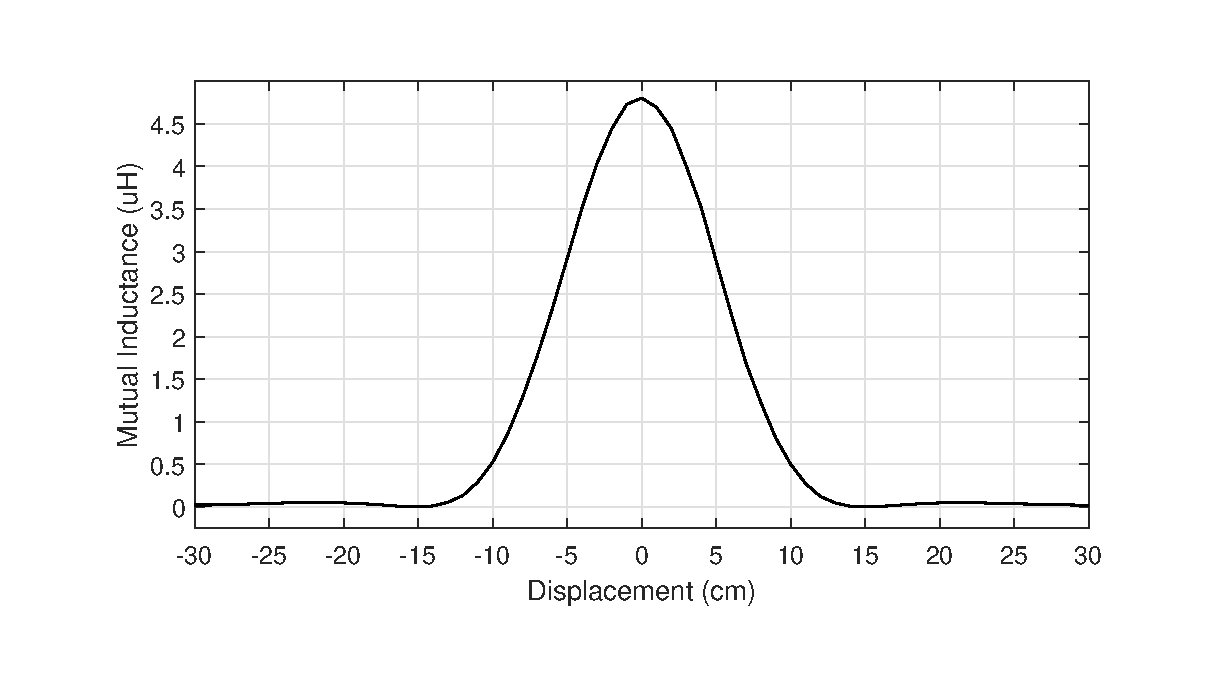
\includegraphics[clip, trim=1.5cm 0.9cm 1cm 0.925cm, width=1\columnwidth]{FIGS/FIG3.eps}
	    \end{center}
	    \vspace{0mm}
	    %\caption{Eigenvalues of the proposed system, with and without the presence of the load.}
	    \caption{Mutual inductance profile when the receiver moves from -31 cm to 31 cm with the reference point of the transmitter aligned position.}
	    \label{FIG3}
	    \vspace{-3mm}
	\end{figure}
	
	%%EQ2
	\begin{flalign}
	    \omega_0=\frac{1}{\sqrt{L_{\mathrm{S}}C_{\mathrm{P}}}}=\frac{1}{\sqrt{C_{\mathrm{T}}\left(L_{\mathrm{TT}}-K_\mathrm{SSF}L_{\mathrm{S}}\right)}}=\frac{1}{\sqrt{L_{\mathrm{RR}}C_{\mathrm{R}}}} &&
	\end{flalign}
    
	\noindent where $\omega_0$ is the tuning frequency of the system and $K_\mathrm{SSF}$ is the soft-switching factor, which is unity for zero phase switching and is ${\pi^2}/{8}$ for zero current switching \cite{pantic}.
	With the use of realistic variations of the transmitter-receiver mutual inductance shown in Fig.~\ref{FIG3}, which is obtained from the laboratory setup with the specifications given in Table~\ref{TBL1}, displacement of the eigenvalues obtained from \eqref{EQ1} are depicted in Fig.~\ref{FIG4}.
	
	%%FIG4
	\begin{figure}
	    \begin{center}
        \subfloat[]{
	            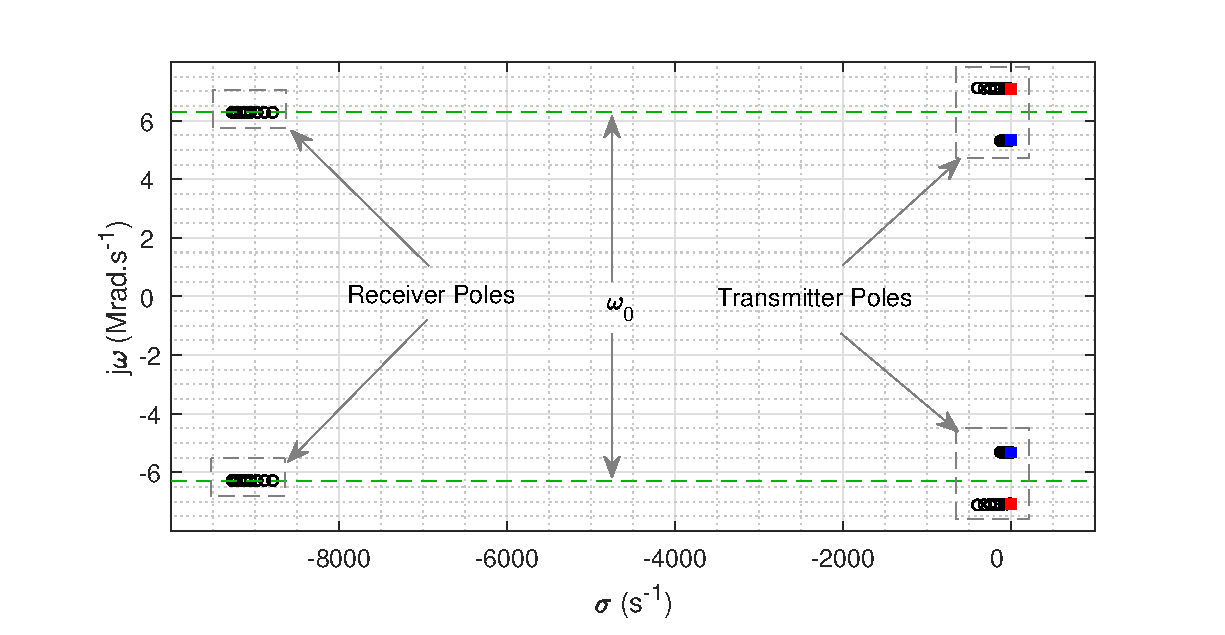
\includegraphics[clip, trim=0.6cm 0cm 1.5cm 0.6cm, width=1\columnwidth]{FIGS/FIG4A.eps}
	    }\\
	    \vspace{-3mm}
	    \subfloat[]{
	            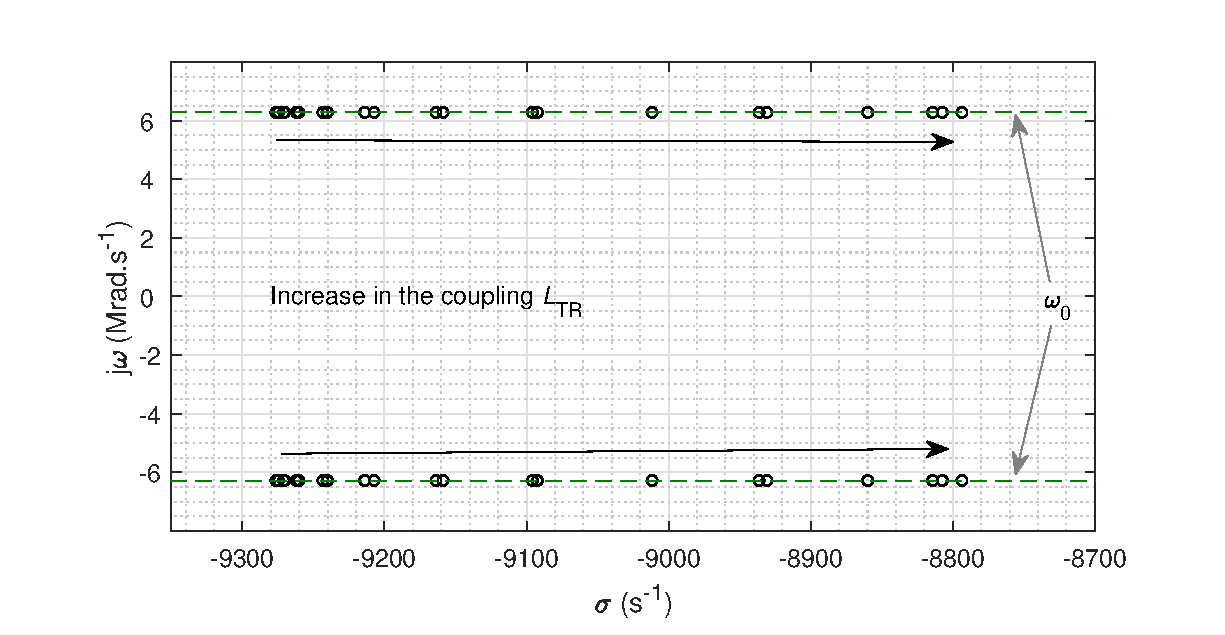
\includegraphics[clip, trim=0.6cm 0cm 1.5cm 0.6cm, width=1\columnwidth]{FIGS/FIG4B.eps}
	    }\\
	    \vspace{-3mm}
	    \subfloat[]{
	            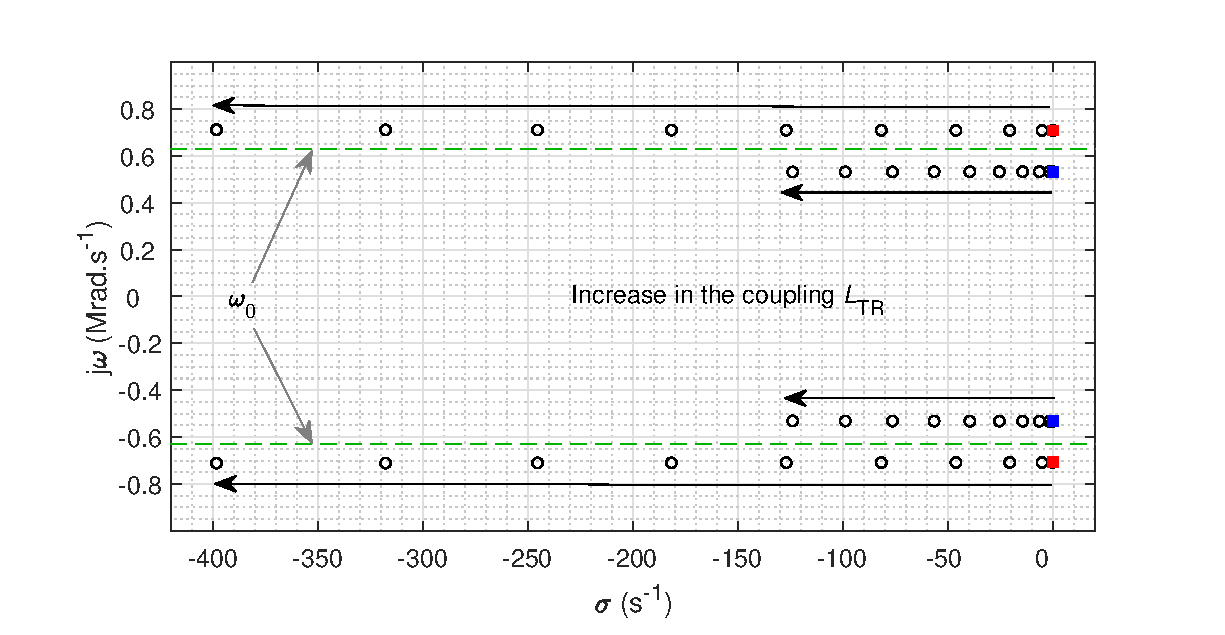
\includegraphics[clip, trim=0.6cm 0cm 1.5cm 0.6cm, width=1\columnwidth]{FIGS/FIG4C.eps}
	    }
	    \vspace{-3mm}
	    \end{center}
	    %\caption{Eigenvalues of the proposed system, with and without the presence of the load.}
	    \caption{Changes of eigenvalues when the coupling in the proposed system changes; (a) overall poles, (b) receiver poles, and (c) transmitter poles.}
	    \label{FIG4}
	    \vspace{-5mm}
	\end{figure}
	
	As it is shown in Fig.~\ref{FIG4}, poles of the transmitter are closer to the $\mathrm{j}\omega$ axis, and as a result they are more influential on the dynamic behavior of the system compared to those of the receiver poles.  Considering the variation of transmitter-receiver mutual inductance shown in Fig.~\ref{FIG3}, the higher the mutual inductance, the further the transmitter poles move away from the vertical axis, and the closer the receiver poles shift towards to the imaginary axis. The occurrence of such a phenomenon is expected, as the higher the power received from the transmitter, the higher the damping factor would be and the transmitter poles move further to the left of the s-plane. In other words, as long as bifurcation does not happen and eigenvalues get closer to each other, damping factor of the system increases, and it makes the system to be more stable. This phenomenon is observable from the Bode diagram of the LCC front-end current ${I}_\mathrm{S}$ to the LCC input voltage ${V}_{\mathrm{in}}$ transfer function ($\mathrm{H'}(s)$) shown in Fig.~\ref{FIG5}, when the transmitter-receiver mutual inductance changes through Fig.~\ref{FIG3} profile \cite{farajizadeh,bif}. {\color{blue}Worthy to mention that similar increase in the bandwidth also occurs between the input signal and other state variables of the system, such as the transmitter current $I_\mathrm{T}$ to the input voltage $V_\mathrm{in}$ transfer function of $\mathit{H}(s)$. However, as this phenomenon is more observable in $\mathrm{H'}(s)$, variations of bandwidth is only depicted for $\mathrm{H'}(s)$.}
    %%FIG5
	\begin{figure}
	    \begin{center}
        \subfloat[]{
	            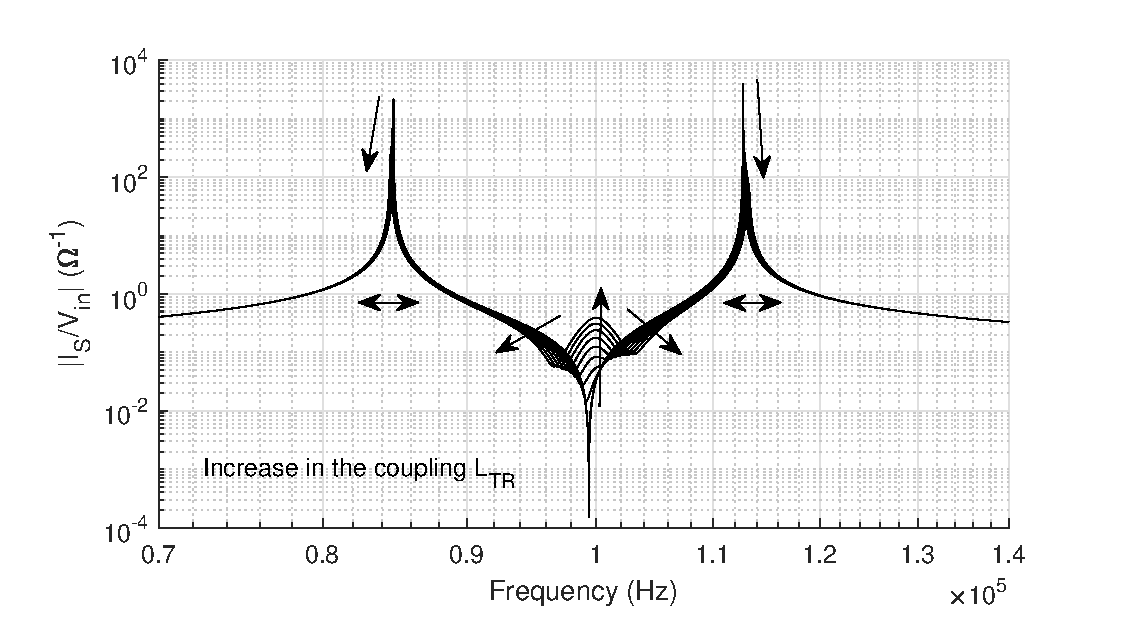
\includegraphics[clip, trim=0.6cm 0cm 1cm 1cm, width=1\columnwidth]{FIGS/FIG5A.eps}
	    }\\
	    \vspace{-3mm}
	    \subfloat[]{
	            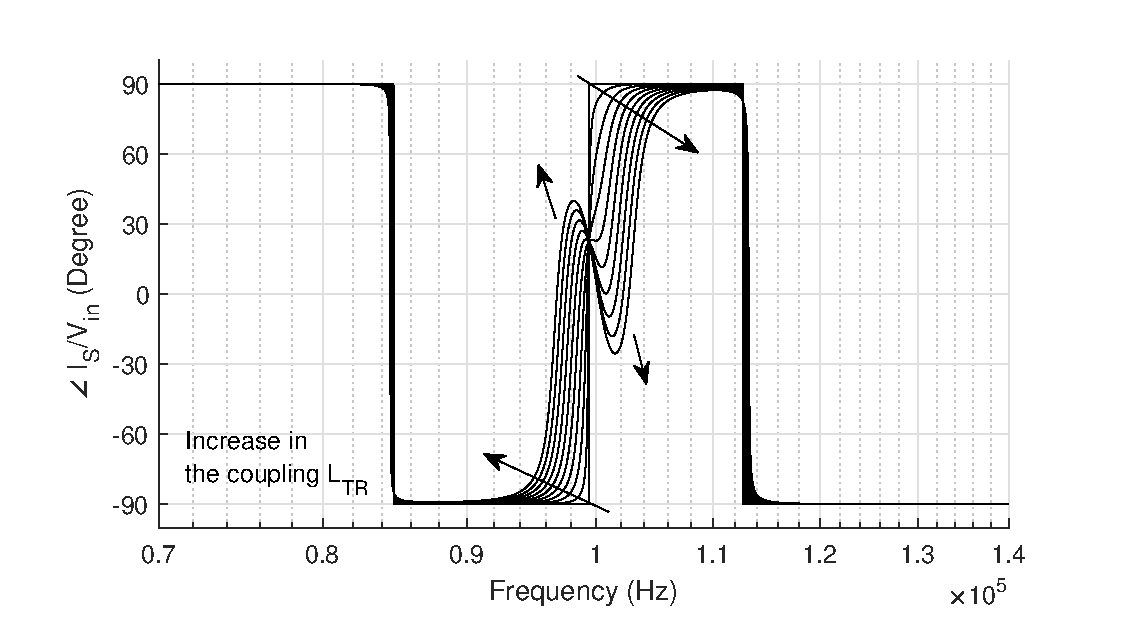
\includegraphics[clip, trim=0.6cm 0cm 1cm 1cm, width=1\columnwidth]{FIGS/FIG5B.eps}
	    }\\
	    \vspace{-3mm}
	    \end{center}
	    %\caption{Eigenvalues of the proposed system, with and without the presence of the load.}
	    \caption{Variation of the bandwidth in the Bode diagram of ${{I}_{\mathrm{S}}}/{{V}_{\mathrm{in}}}$.}
	    \label{FIG5}
	    \vspace{-3mm}
	\end{figure}
	
	Therefore, the worst case of dynamic behavior happens when there is no coupling between the transmitter and receiver. This also simplifies the analysis by removing the receiver part from the WPT system shown in Fig.~\ref{FIG2}. Moreover, to show the effect of ESRs of the transmitter on the dynamic behavior of the system, the influential ESRs, which are related to the source and front end series inductance ($R_\mathrm{S}$) and transmitter ESR ($R_\mathrm{T}$) are considered in the model. As a result, the state-space model of the system can be scaled down as follows.
	
	%%EQ3
	\begingroup
	\small
	\begin{flalign}
	    s\times
	    \underbrace{
	    \begin{bmatrix}
	     {V}_\mathrm{P}\\{V}_\mathrm{T}\\{I}_\mathrm{S}\\{I}_\mathrm{T}   
	    \end{bmatrix}
	    }_\textbf{X}
	    =
	    \underbrace{
	    \begin{bmatrix}
	        -\frac{1}{L_{\mathrm{S}}}    &   0   &   -\frac{R_{\mathrm{S}}}{L_{\mathrm{S}}}   &    0\\
	        \frac{1}{L_{\mathrm{TT}}}     &   -\frac{1}{L_{\mathrm{TT}}}  &   0                 &   -\frac{R_{\mathrm{T}}}{L_{\mathrm{TT}}}\\
	        0     &   0   &   \frac{1}{C_{\mathrm{P}}}                 &   -\frac{1}{C_{\mathrm{P}}}\\
	        0     &   0   &   0                 &   \frac{1}{C_{\mathrm{T}}}
	    \end{bmatrix}
	    }_\textbf{A}
	    \times
	    \underbrace{
	    \begin{bmatrix}
	     {V}_\mathrm{P}\\{V}_\mathrm{T}\\{I}_\mathrm{S}\\{I}_\mathrm{T}    
	    \end{bmatrix}
	    }_\textbf{X}
	   +
	    \underbrace{
	    \begin{bmatrix}
	     \frac{1}{L_{\mathrm{S}}}\\0\\0\\0   
	    \end{bmatrix}
	    }_\textbf{B}
	    \times
	    \underbrace{
	    {V}_{\mathrm{in}}
	    }_\textbf{U} &&
	    \label{EQ3}
	\end{flalign}
	\endgroup
	
	Equation \eqref{EQ3} is considered as the simplified model of the system, and in the next section it is shown how the implementation of the vertically shifted model of the system helps designing a simplified controller to stabilize the system.
	
	\section{Asymmetric Envelope Transfer Function}
	In this section, it is shown how the envelope transfer function of a linear system can be obtained. Using this concept, the dynamic behavior of the system around a specific frequency of operation can be modelled. This approach is especially useful when the amplitude of the oscillating output is to be observed and controlled, as shown in Fig.~\ref{FIG6}.

	%%FIG6
	\begin{figure}
	    \begin{center}
                \subfloat[]{
	                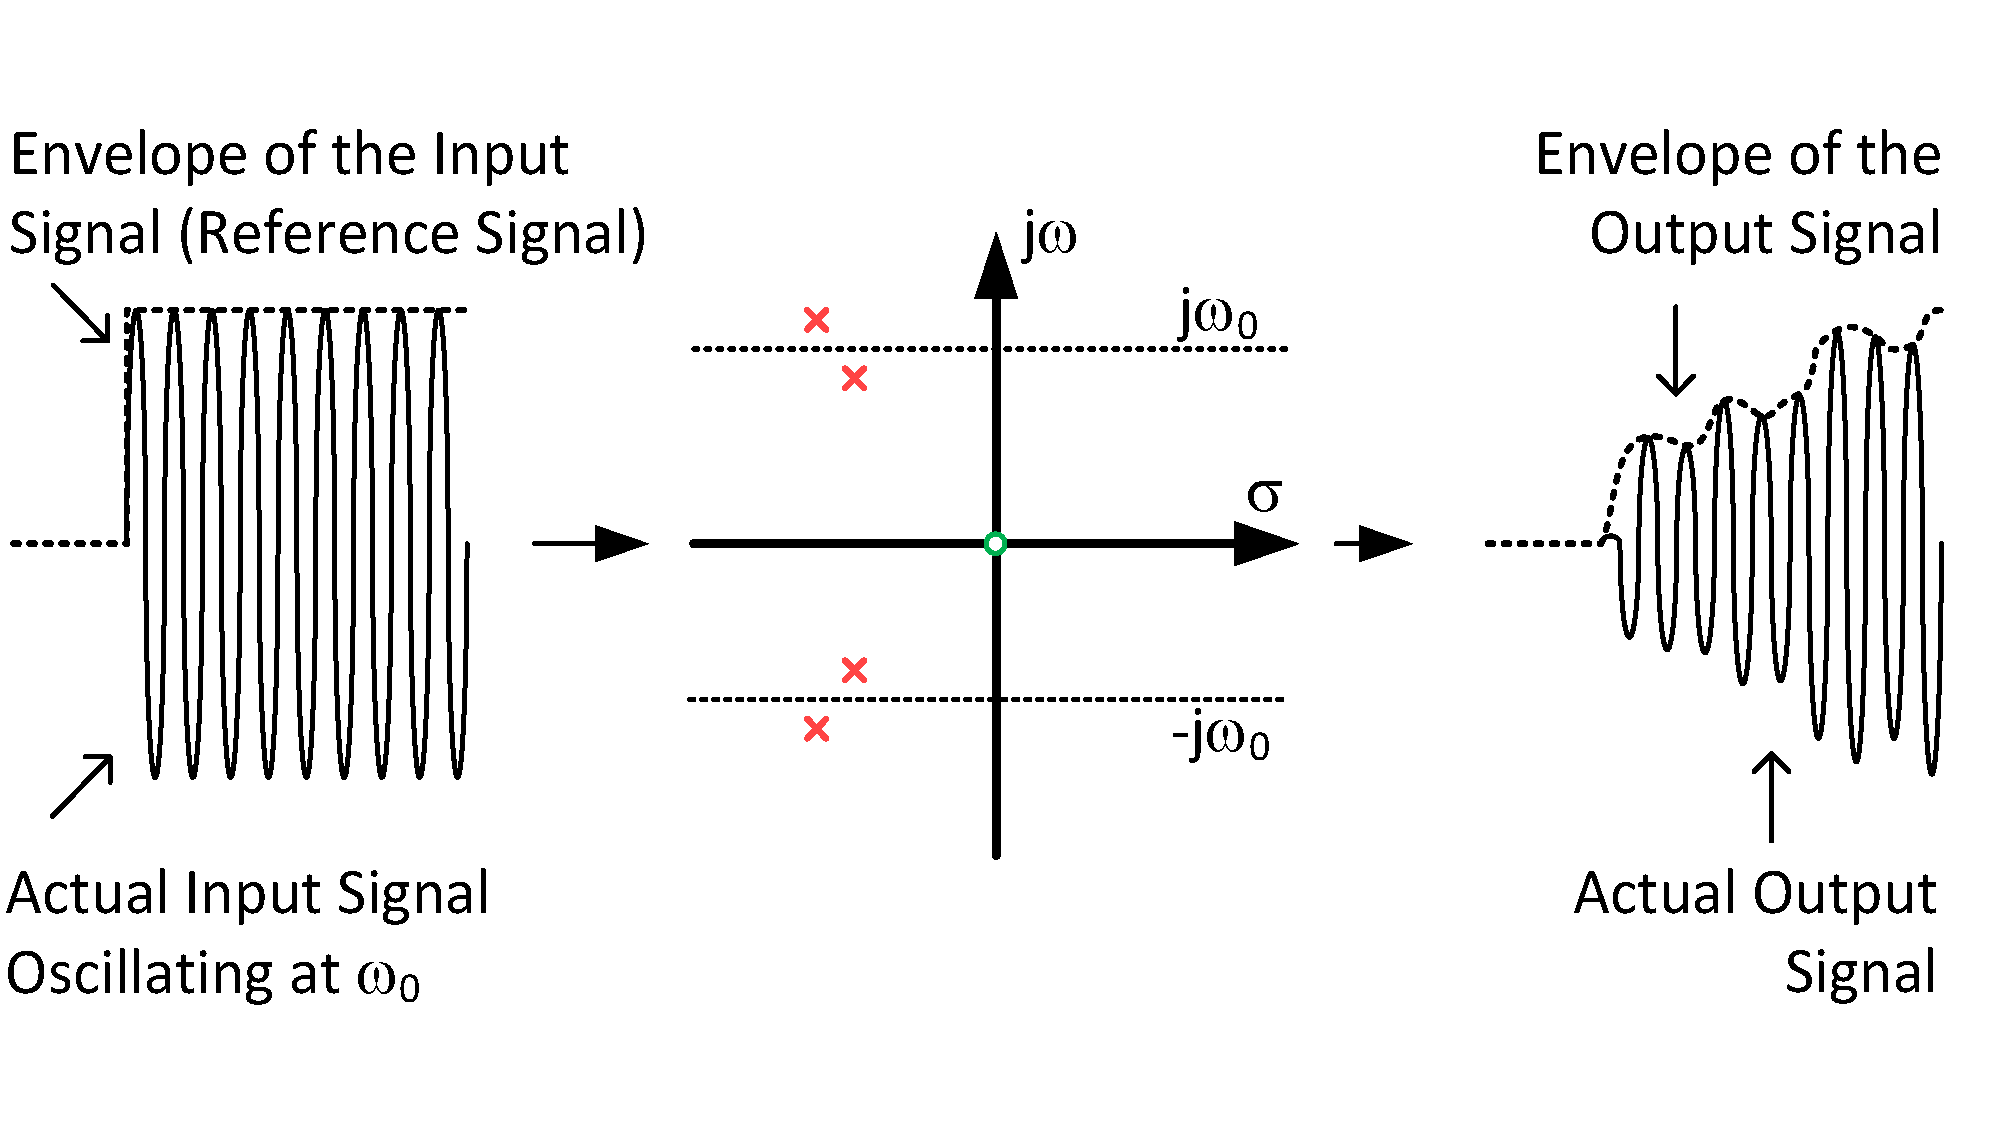
\includegraphics[clip, trim=0cm 2cm 0cm 2cm, width=1\columnwidth]{FIGS/FIG6A.pdf}
	            }\\
	           % \vspace{-5mm}
	            \subfloat[]{
	                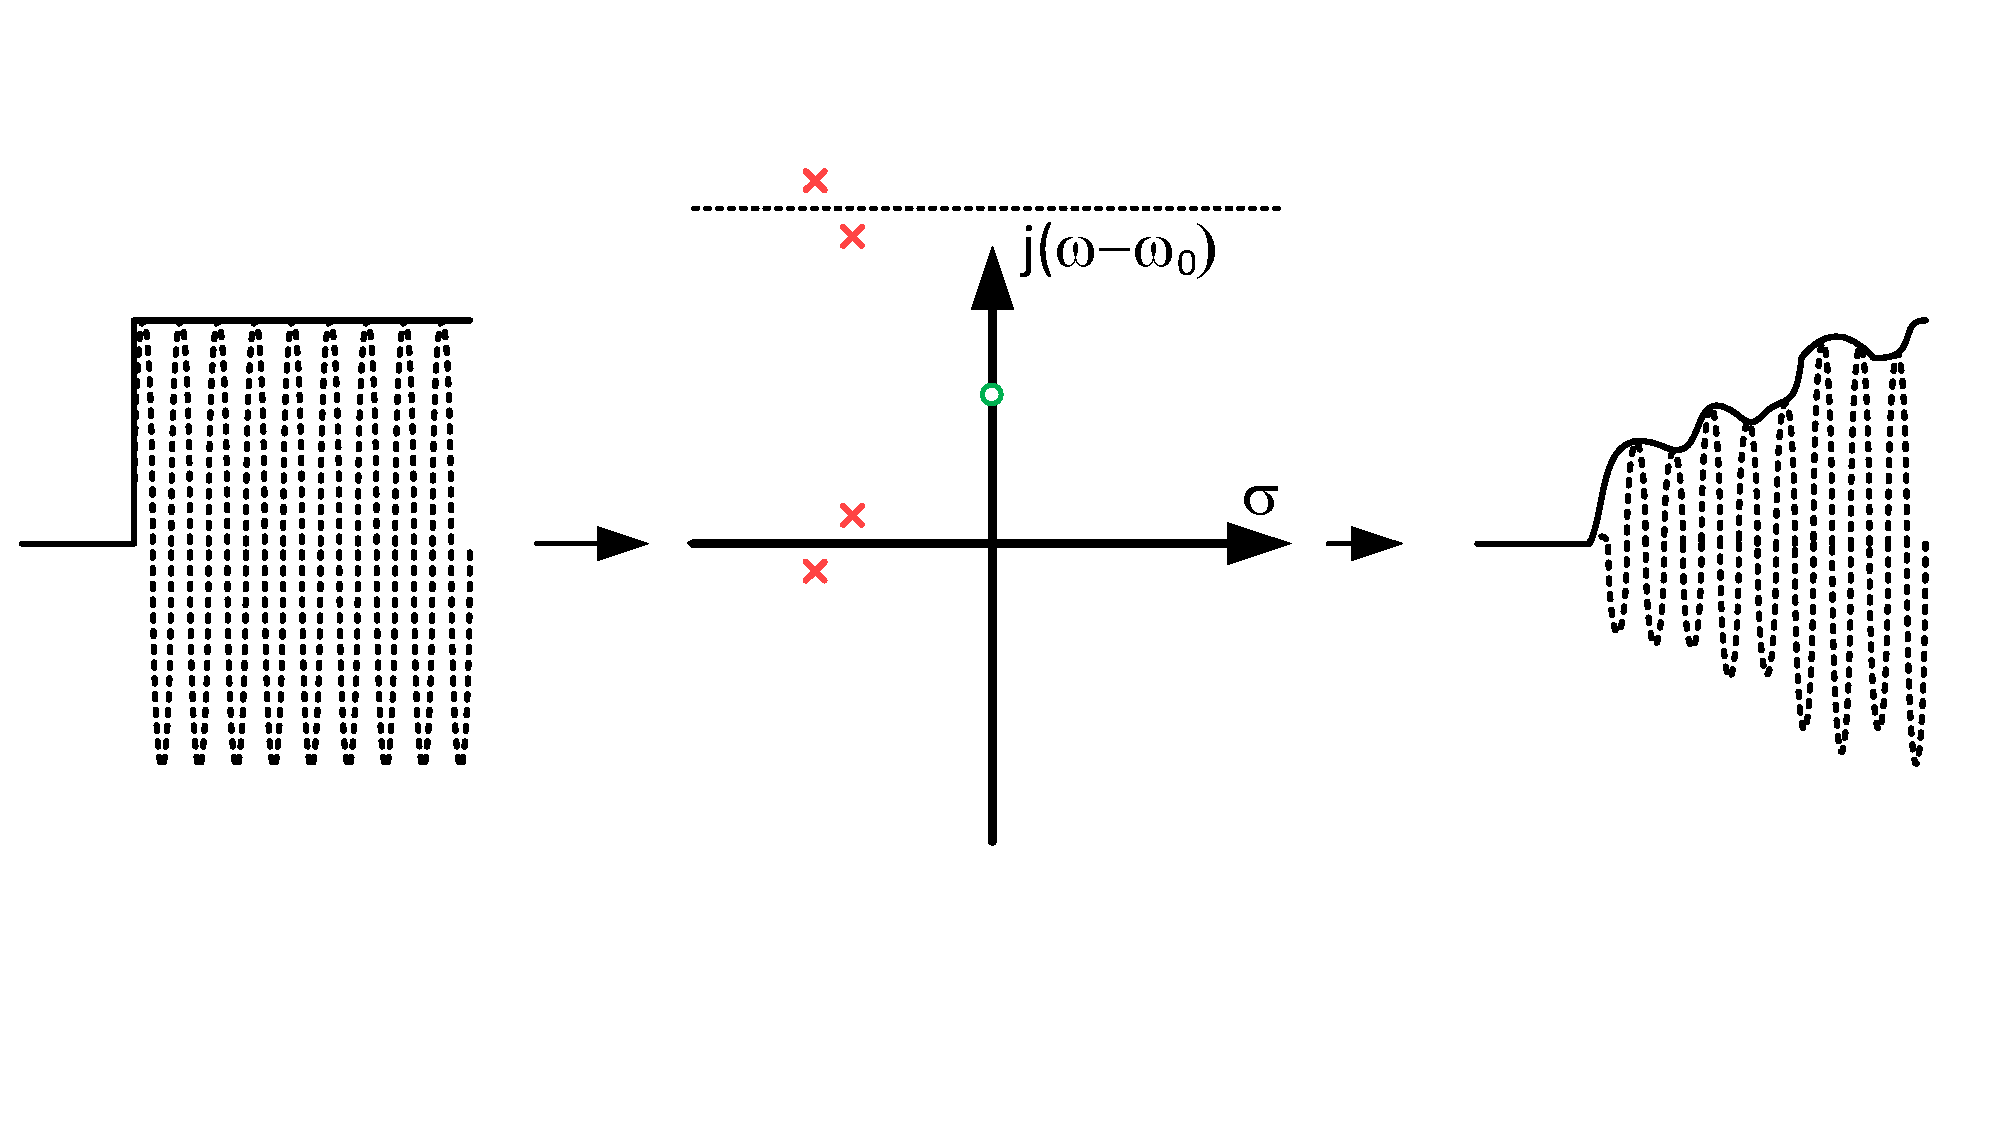
\includegraphics[clip, trim=0cm 4cm 0cm 2cm, width=1\columnwidth]{FIGS/FIG6B.pdf}
	            }\\
	           % \vspace{-5mm}
	            \subfloat[]{
	                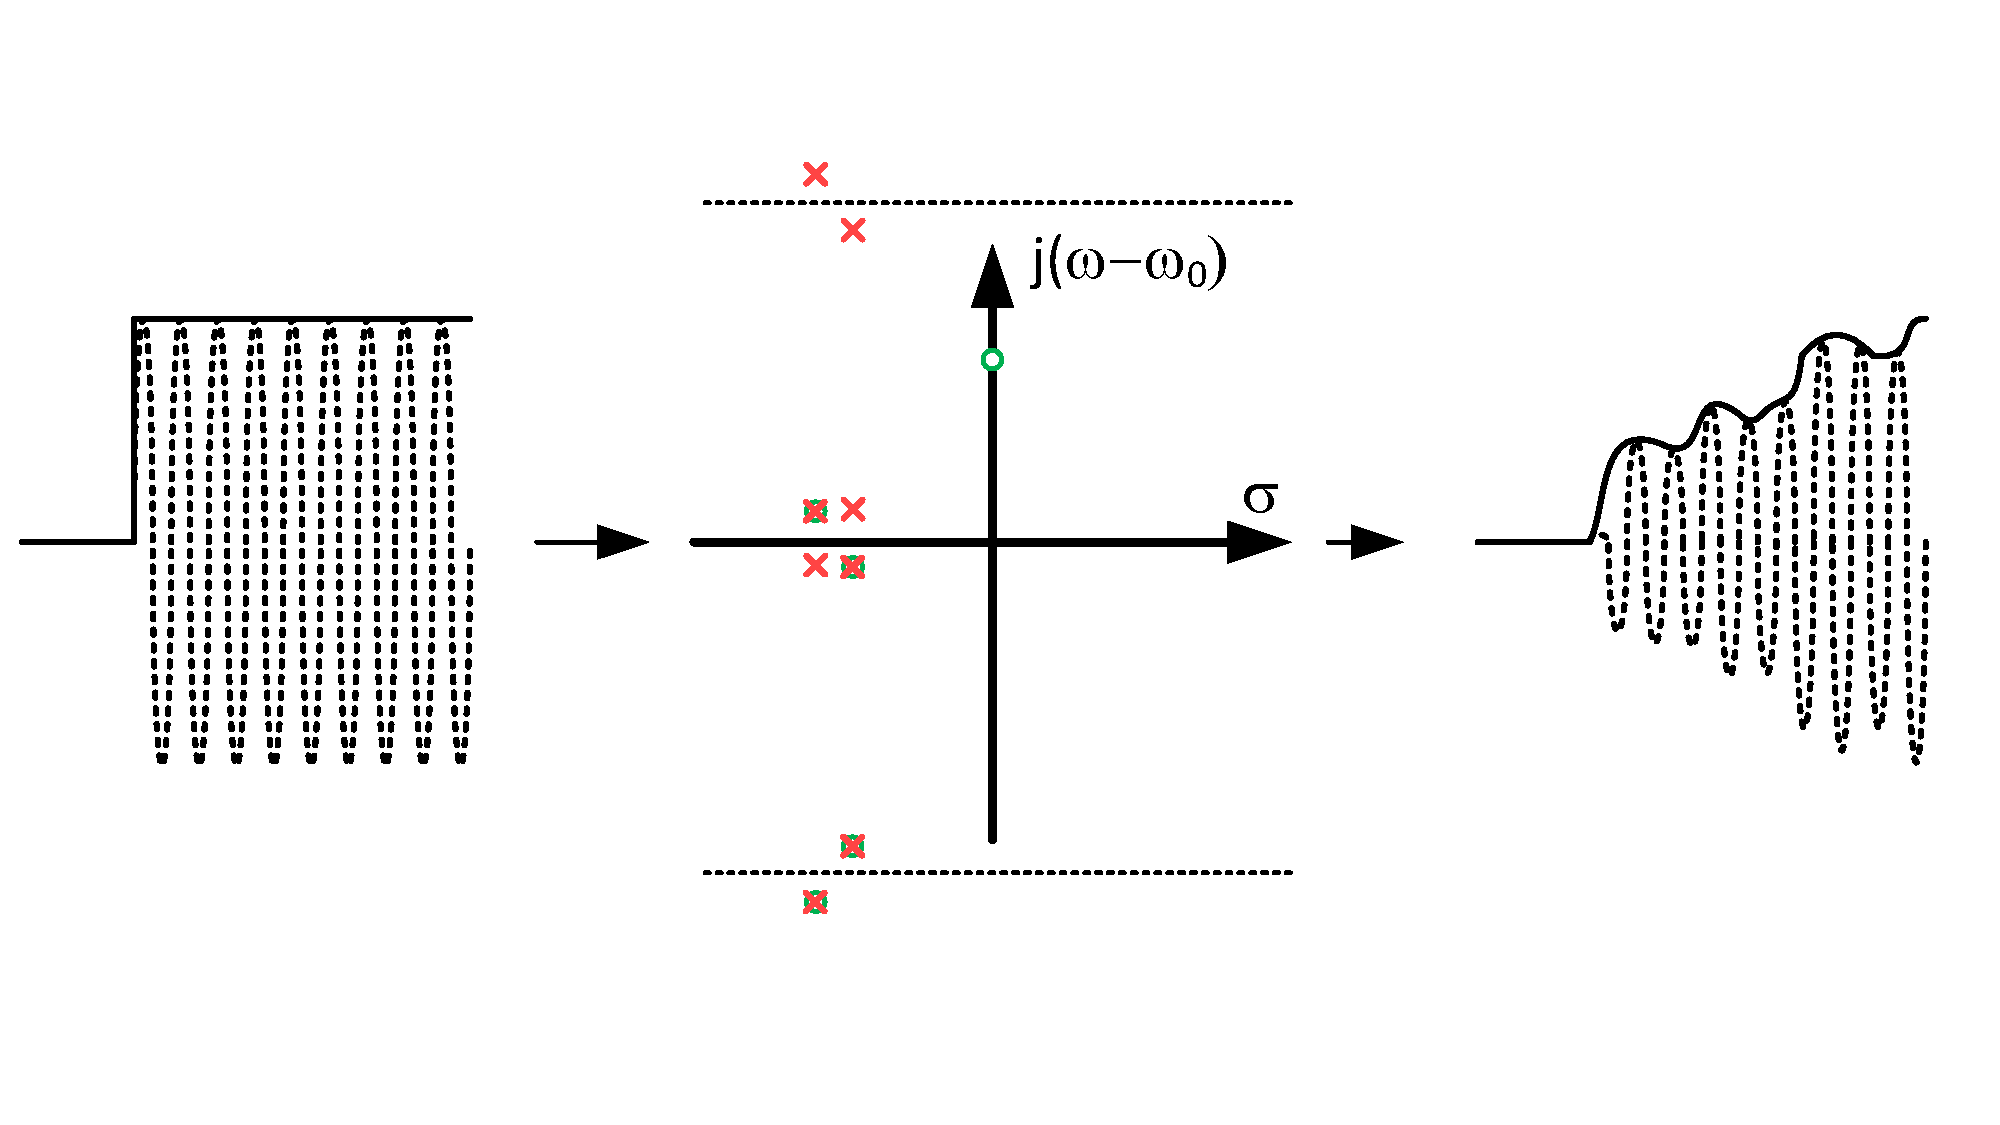
\includegraphics[clip, trim=0cm 2cm 0cm 2cm, width=1\columnwidth]{FIGS/FIG6C.pdf}
	            }\\
	    \vspace{-3mm}
	    \end{center}
	    %\caption{Eigenvalues of the proposed system, with and without the presence of the load.}
	    \caption{Vertically shifted model of a multi-order system; (a) actual poles (o) and zeros (x), (b) vertically shifted model with the reference of operating frequency of $\omega_0$, and (c) asymmetric vertically shifted transfer function after multiplying the denominator by the complex conjugate of the asymmetric poles.}
	    \label{FIG6}
	    \vspace{-3mm}
	\end{figure}
	
	Towards this end, s-parameter in \eqref{EQ3} is vertically shifted to either $\mathrm{j}\omega_0$ or $-\mathrm{j}\omega_0$. By extracting $\mathit{H}(s)$, a transfer function that links the input $V_\mathrm{in}$ to the output $I_\mathrm{T}$ from \eqref{EQ3} can be represented as in \eqref{EQ4}. 
	%%EQ4
	\begin{flalign}
	    \mathit{H}(s)=\frac{I_\mathrm{T}}{V_\mathrm{in}}=\mathrm{G}\frac{\mathrm{N}(s)}{\mathrm{D}(s)} &&
	    \label{EQ4}
	\end{flalign}
	
 	\noindent where $\mathrm{N}(s)=\prod_{i=1}^{m}(s+z_i)$, $\mathrm{D}(s)=\prod_{i=1}^{n}(s+p_i)$, and $\mathit{H}(s)$ is strictly proper ($n>m$). To obtain the vertically shifted transfer function from $\mathit{H}(s)$, the analytical reference point of s-plane is changed from the origin of the s-plane to the operating frequency of $\omega_0$. For this purpose, $s$ in the original transfer function of the system $\mathit{H}(s)$ is replaced by $s-\mathrm{j}\omega_0$ to form $\mathit{H}(s-\mathrm{j}\omega_0)$ as given in \eqref{EQ5}. Figs.~\ref{FIG6}(a) and (b) show the actual and vertically shifted s-plane zeros and poles of a multi-order system respectively.
 	%%EQ5
	\begin{flalign}
	    \mathfrak{H}(s)=\mathit{H}(s-\mathrm{j}\omega_0)=\mathrm{G}\frac{\prod_{i=1}^{m}(s+z_i-\mathrm{j}\omega_0)}{\prod_{i=1}^{n}(s+p_i-\mathrm{j}\omega_0)} &&
	    %=\mathfrak{H}_\mathrm{R}(s)+\mathrm{j}\mathfrak{H}_\mathrm{I}(s)&&
	    \label{EQ5}
	\end{flalign}

	The obtained transfer function $\mathfrak{H}(s)$ has real ($\mathfrak{H}_\mathrm{R}(s)$) and imaginary ($\mathfrak{H}_\mathrm{I}(s)$) parts. $\mathfrak{H}_\mathrm{R}(s)$ and $\mathfrak{H}_\mathrm{I}(s)$ can be obtained by multiplying the numerator and denominator of $\mathfrak{H}(s)$ by the complex conjugate of its denominator, as given in \eqref{EQ6}. 
	%%EQ6
	\begin{flalign}
	    \mathfrak{H}(s)=\mathrm{G}\frac{\prod_{i=1}^{m}(s+z_i-\mathrm{j}\omega_0)\prod_{i=1}^{n}(s+p_i+\mathrm{j}\omega_0)}{\prod_{i=1}^{n}(s+p_i-\mathrm{j}\omega_0)\prod_{i=1}^{n}(s+p_i+\mathrm{j}\omega_0)} &&
	    %\label{EQ6}
	    \nonumber
	\end{flalign}
		\begin{flalign}
	    %\mathfrak{H}(s)=\mathit{H}(s-\mathrm{j}\omega_0)=\mathrm{G}\frac{\prod_{i=1}^{m}(s+z_i-\mathrm{j}\omega_0)}{\prod_{i=1}^{n}(s+p_i-\mathrm{j}\omega_0)}
	    =\mathfrak{H}_\mathrm{R}(s)+\mathrm{j}\mathfrak{H}_\mathrm{I}(s)&&
	    \label{EQ6}
	\end{flalign}	

	%%EQ7
 	 \begin{figure*}[b!]
 	 \vspace{-3mm}
	 \begingroup
	 \small
	 \begin{flalign}
	 \mathit{H}(s)=\frac{1}{C_{\mathrm{P}}L_{\mathrm{S}}L_{\mathrm{TT}}}
	 \left(
	 \frac{s}{s^4+
	 \left({\frac{1}{Q_{\mathrm{S}}}}+\frac{1}{Q_{\mathrm{T}}}\right)\omega_0 s^3
	 +\left({2+{\left(1-K_\mathrm{SSF}\right)}{\frac{L_{\mathrm{S}}}{L_{\mathrm{TT}}}}}\right)\omega_0^2 s^2
	 +\left(1+{\left(1-K_\mathrm{SSF}\right)}{\frac{L_{\mathrm{S}}}{L_{\mathrm{TT}}}}{{\frac{1}{Q_{\mathrm{S}}}}}+{\frac{1}{Q_{\mathrm{T}}}}\right)\omega_0^3 s
	 +\left(1-K_\mathrm{SSF}\frac{L_{\mathrm{S}}}{L_{\mathrm{TT}}}\right)\omega_0^4}
	 \right)&&
	 \label{EQ7}
	 \end{flalign}
 	 \vspace{-5mm}
 	 \endgroup
 	 \end{figure*}
	
	In this way, the asymmetric transfer function $\mathfrak{H}(s)$ can be explained in two symmetric real ($\mathfrak{H}_\mathrm{R}(s)$) and imaginary ($\mathfrak{H}_\mathrm{I}(s)$) parts. Figs.~\ref{FIG6}(c) shows the resultant zeros and poles after multiplying the numerator and denominator of $\mathfrak{H}(s)$ by the complex conjugate of its denominator.
	%% FORMER EQ7

    %% FIG7
	 	\begin{figure}[t!]
	 	\begin{center}
	                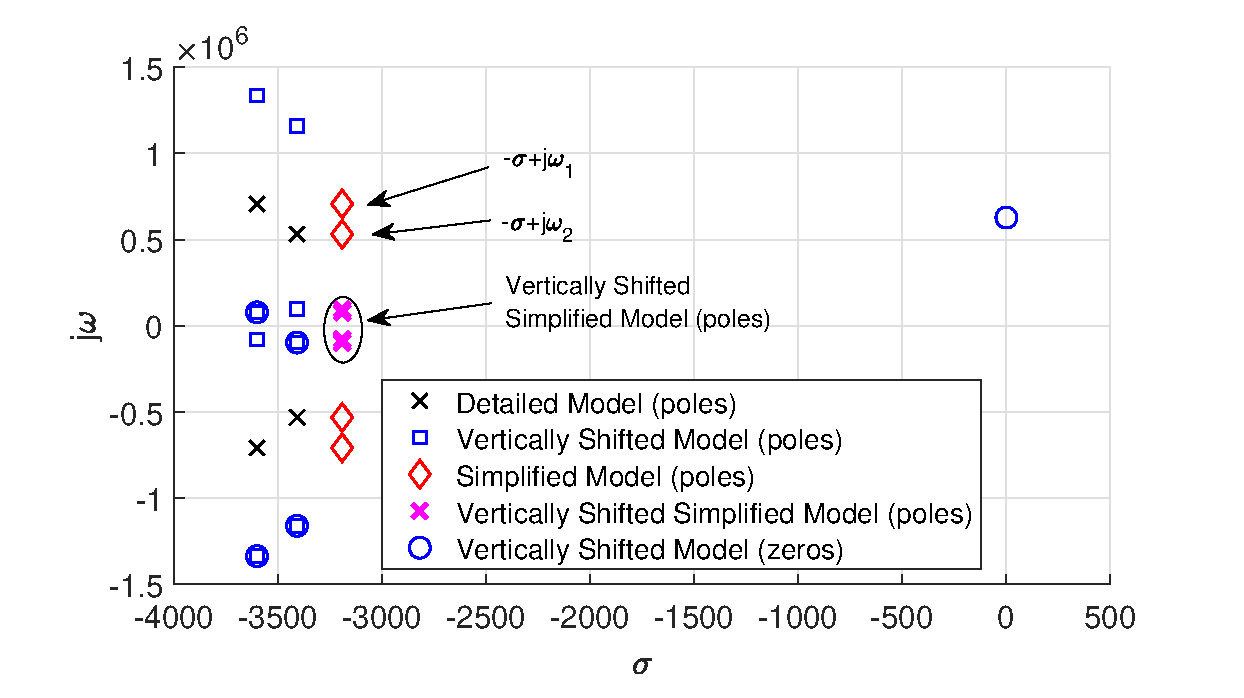
\includegraphics[clip, trim=2mm 0cm 0.5cm 0cm, width=1\columnwidth]{FIGS/FIG7_POLES.eps}
	    \end{center}
	    %\caption{Eigenvalues of the proposed system, with and without the presence of the load.}
	    \vspace{-3mm}
	    \caption{Zeros and poles obtained from the detailed and approximated models.}
	    \label{FIG7}
	    \vspace{-3mm}
	\end{figure}

	  %% FIG9
	 	\begin{figure} [t]
	    \begin{center}
	    \vspace{3mm}
                \subfloat[]{
	                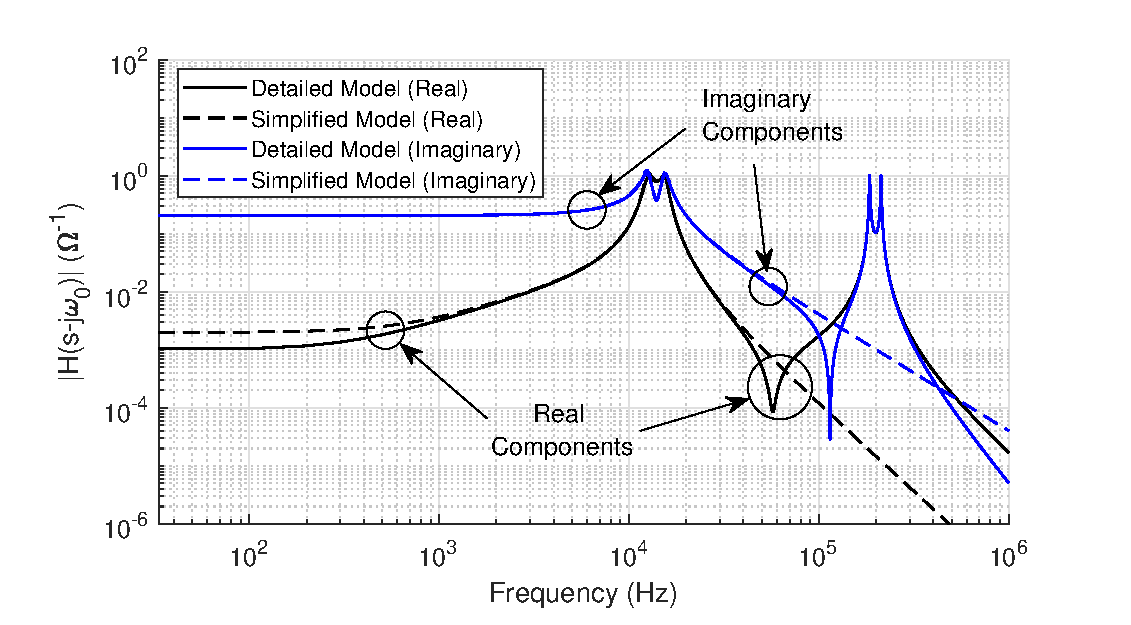
\includegraphics[clip, trim=0.5cm 0 cm 0.5cm 0.5cm, width=1\columnwidth]{FIGS/FIG9A.eps}
	            }\\
	            \vspace{-3mm}
	            \subfloat[]{
	                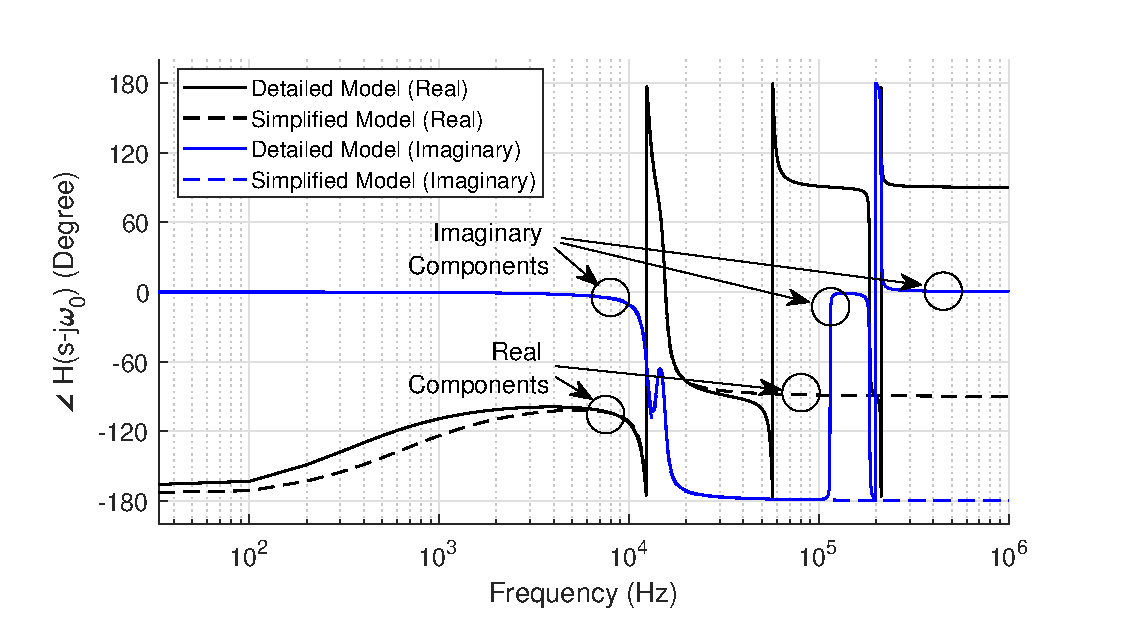
\includegraphics[clip, trim=0.5cm 0cm 0.5cm 0.5cm, width=1\columnwidth]{FIGS/FIG9B.eps}
	            }\\
	    \end{center}
	    %\caption{Eigenvalues of the proposed system, with and without the presence of the load.}
	    \vspace{-3mm}
	    \caption{Bode diagram of $\mathfrak{H}_\mathrm{R}(\mathrm{j}\omega)$ and $\mathfrak{H}_\mathrm{I}(\mathrm{j}\omega)$; (a) amplitude, (b) angle.}
	    \label{FIG9}
	    \vspace{-3mm}
	\end{figure}
	
		 %% FIG10
	 	\begin{figure}[t]
	    \begin{center}
	                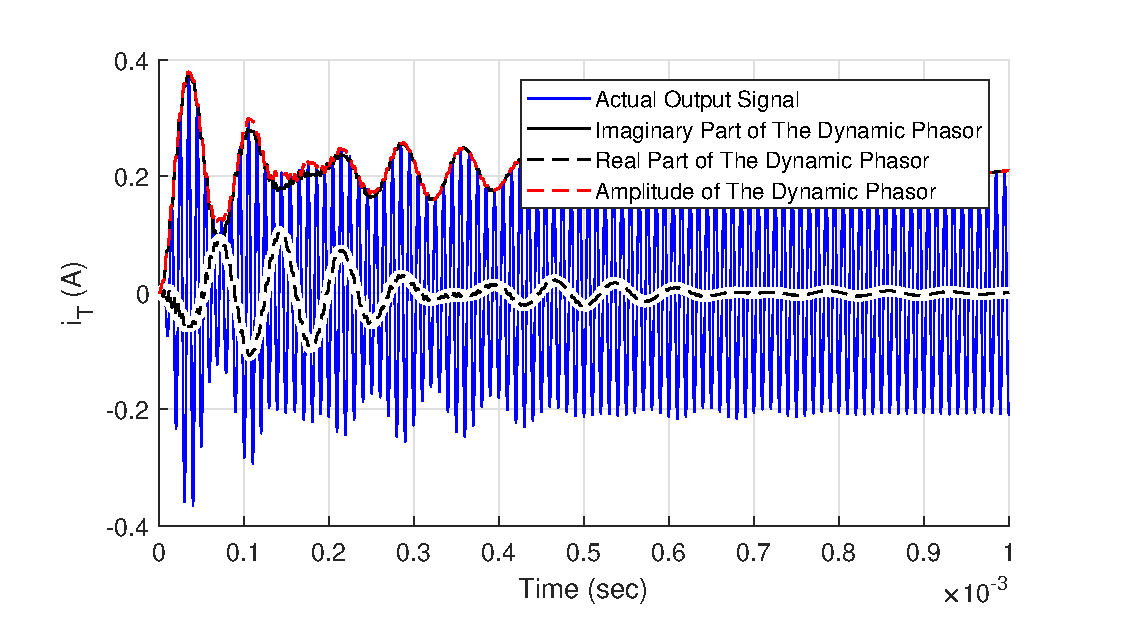
\includegraphics[clip, trim=0.5cm 0cm 0.5cm 0cm, width=1\columnwidth]{FIGS/FIG10.eps}
	    \end{center}
	    %\caption{Eigenvalues of the proposed system, with and without the presence of the load.}
	    \vspace{-3mm}
	    \caption{Step response of amplitude for the LCC front-end loop current $i_{\mathrm{T}}$ for its time-domain behavior and the amplitude of its dynamic phasor (envelope).}
	    \label{FIG10}
	    \vspace{-3mm}
	\end{figure}


	 Therefore, the concerned system can be written in terms of two real $\mathfrak{H}_\mathrm{R}(s)$ and imaginary $\mathfrak{H}_\mathrm{I}(s)$ parts. These transfer functions are the real and imaginary parts of the steady-state gain of $\mathit{H}(\mathrm{j}\omega_0)$ when the dynamics around the frequency of concern ($\omega_0$) is considered. Therefore, $\mathfrak{H}(0)=\mathit{H}(\mathrm{j}\omega_0)$, and $\mathfrak{H}(s)$ resembles the dynamic complex gain that links the envelope of the output signal ($i_\mathrm{T}$) to the envelope of the input signal ($v_\mathrm{in}$). As a result, the amplitude of the step response of $\mathfrak{H}(s)$ is the envelope of the output signal, as shown in Fig.~\ref{FIG6}. For the given LCC network shown in Fig.~\ref{FIG2}, $\mathit{H}(s)={I}_{\mathrm{T}}/{V}_{\mathrm{in}}$ can be obtained as in \eqref{EQ7}. In this equation, $Q_\mathrm{S}={L_{\mathrm{S}}\omega_0}/{R_{\mathrm{S}}}$ and $Q_\mathrm{T}={L_{\mathrm{TT}}\omega_0}/{R_{\mathrm{T}}}$ are the quality factors of the LCC front-end inductance and the transmitter coil respectively.
	 
	 Although the order of the resultant complex transfer function $\mathfrak{H}(s)$ is double the original transfer function $\mathit{H}(s)$, some poles and zeros are shifted way far away from the operating frequency $\omega_0$, and they can be approximated by their steady state behavior at $\omega_0$ (e.g. $(s+\sigma_1-\mathrm{j}(\omega_1+\omega_0))\rightarrow(\sigma_1-\mathrm{j}(\omega_1+\omega_0))$). Moreover, if the quality factor of the system is high enough, the real component of the uninfluential poles and zeros can also be neglected (e.g.
	 $(\sigma_1-\mathrm{j}(\omega_1+\omega_0))\rightarrow(-\mathrm{j}(\omega_1+\omega_0))$).
	 If the system needs to be further simplified, the uninfluential zeros and poles can be removed altogether as shown in Appendix.
	 
	 For the specifications given in Table~\ref{TBL1}, the zeros and poles obtained from the detailed and simplified models are shown in Fig.~\ref{FIG7}. For the specified system, 
	 % the Bode diagrams of $\mathfrak{H}(s)$ and its real and imaginary components are shown in Figs.~\ref{FIG8} and \ref{FIG9} respectively.
	 Bode diagrams of the real and imaginary components of $\mathfrak{H}(s)$ are shown in Fig.\ref{FIG9}. Referring to Fig.~\ref{FIG9}, it is clear that the simplified transfer functions of $\mathfrak{H}_\mathrm{R}(s)$ and $\mathfrak{H}_\mathrm{I}(s)$ can be effectively used for frequencies below  $15~\mathrm{kHz}$. 
	 Worthy to mention that simplified equations given in the appendix can also be used to reduce the order of $\mathfrak{H}_\mathrm{R}(s)$ and $\mathfrak{H}_\mathrm{I}(s)$; however, from here onwards, to make sure that the dynamic behavior of the system is completely modeled, the detailed transfer functions are used to analyze the system and design the controller. 
	 
	 To have some intuition about the time-domain behavior of the detailed $\mathit{H}(s)$ and $\mathfrak{H}(s)$, an input oscillating variable with a step change in its amplitude ($v_\mathrm{in}=A_\mathrm{m}\mathrm{u}(t)\sin{(\omega_0 t)}$; $f_0=\mathrm{100~\mathrm{kHz}}$, $A_\mathrm{m}=1~\mathrm{V}$) is applied to the detailed model of the concerned system $\mathit{H}(s)$, and its resultant influence on the output variable $i_\mathrm{T}$ is compared with the step response of its vertically shifted model $\mathfrak{H}(s)$ when it is fed by $V_\mathrm{in}(t)=A_\mathrm{m}\mathrm{u}(t)$ in Fig.~\ref{FIG10}. The input and output signals of the vertically shifted model $\mathfrak{H}(s)$ can be called dynamic phasors.
	 
	 One of the advantages of the vertically shifted model is to find the dominant orientation of the system, {\color{red}which is $\arctan(\mathfrak{H}_\mathrm{I}(s)/\mathfrak{H}_\mathrm{R}(s))$}, to its real or imaginary transfer functions at different frequencies. As it can be seen in 
	 %Figs.~\ref{FIG8} and \ref{FIG9}
	 Fig.~\ref{FIG9}, $\mathfrak{H}_\mathrm{I}(s)$ is considerably larger than $\mathfrak{H}_\mathrm{R}(s)$ before $5~\mathrm{kHz}$. Nonetheless, $\mathfrak{H}_\mathrm{R}(s)$ component gets closer to $\mathfrak{H}_\mathrm{I}(s)$ somewhere around $15~\mathrm{kHz}$ and $200~\mathrm{kHz}$. It means, on the one hand, $\mathfrak{H}_\mathrm{I}(s)$ can be a reasonable approximation of $\mathfrak{H}(s)$ when the operating frequency is less than $5~\mathrm{kHz}$. On the other hand, if the amplitude fluctuations of the oscillating input signal approaches the extreme frequencies, such as $15~\mathrm{kHz}$ and $200~\mathrm{kHz}$, $\mathfrak{H}_\mathrm{I}(s)$ cannot accurately follow the entire behavior of the system. 
	 
	 Comparing the resultant imaginary part of the dynamic phasor with its amplitude in Fig.~\ref{FIG10}, this deviation is observable at the beginning of the step response transients. During this time, the real part of the dynamic phasor has a significant amplitude, and it oscillates at a frequency around $15~\mathrm{kHz}$ which is close to the peak of the $\left|\mathfrak{H}_\mathrm{R}(s)\right|$ (and $\left|\mathfrak{H}_\mathrm{I}(s)\right|$) in their Bode diagrams shown in Fig.~\ref{FIG9}. 
	 Digital sampling and the presence of the close-loop controllers usually introduce an effective bandwidth to the resultant system frequency response. Hence, with the use of an appropriate controller, the frequency response of the closed loop system can be appropriately shaped in such a way that the imaginary transfer function $\mathfrak{H}_\mathrm{I}(s)$ provides a close approximation to the actual transfer function $\mathfrak{H}(s)$. complex orientation of the plant remains constant, the system effectively follows the dominant orientation. 
	 In the next section, the sampling technique required to observe the dominant behaviour (orientation) of the system {\color{red}using the proposed technique of vertically shifted transfer function is examined}.
	 
	 \section{Single-Oriented PWM-Synchronized Sampling Technique}
	 Fig.~\ref{FIG11} shows the generic closed-loop block-diagram of the sampled system to stabilize dynamic transients of the vertically shifted model of the system. With this end in view, the dynamic phasor of the direct ($Y_\mathrm{R}$) and quadrature ($Y_\mathrm{I}$) output components are to be sampled and fed back to the controller. Aiming to reduce the complexity of the controller, decreasing the sampling rate, and removing the undesirable delay of the low-pass filters, taking the samples from the dominant orientation of the system is carried out by the proposed SOPWMS2 technique. In the following, this technique is explained.
	 
	 %% FIG11
	 \begin{figure}
	     \centering
	     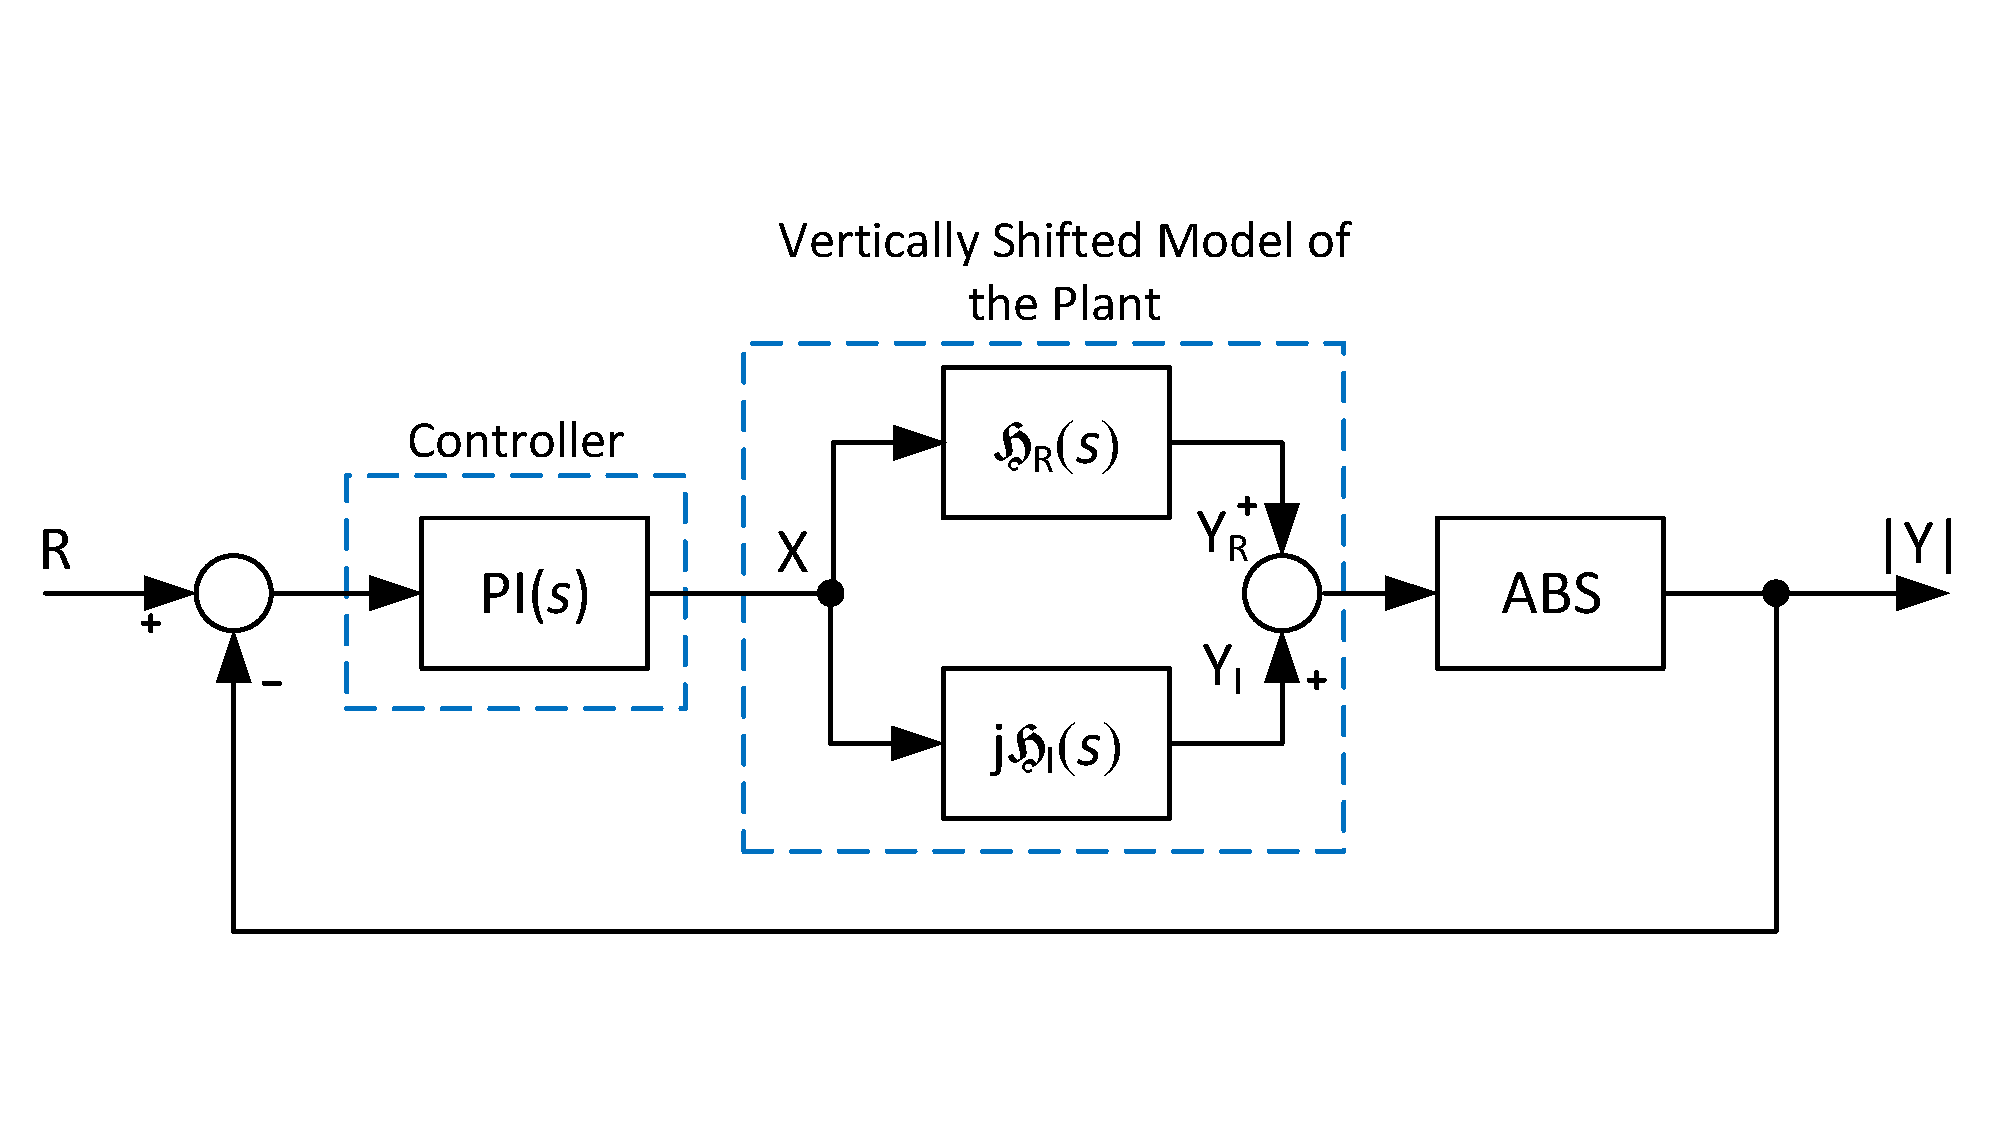
\includegraphics[clip, trim=0cm 2.5cm 0cm 2.5cm, width=1\columnwidth]{FIGS/FIG11.pdf}
	     \vspace{-5mm}
	     \caption{Generic close-loop controller to stabilize the verticaly shifted model of the plant.}
	     \label{FIG11}
	     \vspace{0mm}
	 \end{figure}
	 
	  To derive the dynamic phasor with the proposed PWM-synchronized sampling technique, sampling instants (interrupts) should be synchronized with the reference signal. The reference signal can be generated internally or externally. When the reference signal is externally made (e.g. taking the voltage from the point of common coupling in a network as a reference variable), synchronization can be achieved by a PLL \cite{PLL}. Nonetheless, when the reference signal is internally made (e.g. taking output voltage of a converter, which is made by the controller PWM signals, as a reference signal), synchronization can be easily done with the use of PWM signals that generate the reference signal $v_{\mathrm{in}}$. %Fig.~\ref{FIG12} shows an example of the sampling interrupts which are synchronized by the PWM signal. 
	  
	  Taking the reference signal of $x$ given in \eqref{EQ8} as an example, it can be proved that other output signals of the system, such as $y$ can be represented as in \eqref{EQ9}.
	 %EQ8
	 \begin{flalign}
	    x=X_{\mathrm{in}}(t)\cos(\omega_0t) &&
	    \label{EQ8}
	\end{flalign}
	 %EQ9
	 \begin{flalign}
	    y=Y(t)\cos(\omega_0t+\psi)   &&
	    \label{EQ9}
	\end{flalign}
	 
	 Therefore, the dynamic phasor $Y(t)$ can be mapped on two orthogonal pairs of real $Y_\mathrm{R}(t)$ and imaginary $Y_\mathrm{I}(t)$ time varying components in the following way.
	  %EQ10
	 \begin{flalign}
	    y=Y_\mathrm{R}(t)\cos(\omega_0t)+Y_\mathrm{I}(t)\sin(\omega_0t)   &&
	    \label{EQ10}
	\end{flalign}
	 From \eqref{EQ10}, it is clear that the amplitude (envelope) of the output signal can be obtained as follows.
	  %EQ11
	 \begin{flalign}
	    \left|Y(t)\right|=\sqrt{Y_\mathrm{R}^2(t)+Y_\mathrm{I}^2(t)}   &&
	    \label{EQ11}
	\end{flalign}
	
	 The real part $Y_\mathrm{R}(t)$ is in-phase with the reference signal $v_\mathrm{in}(t)$, and $Y_\mathrm{I}(t)$ {\color{red}leads} by $90^\circ$. This means that the dynamic phasor of the output signal can be digitally reconstructed by taking proper samples synchronized by the input signal $x$. Fig.~\ref{FIG12} shows how taking samples at the moments of PWM zero crossing (``I"), and PWM mid-points (``R"), PWM-synchronized sampling technique can effectively retrieve the envelope of the output signal $i_\mathrm{T}$ at the time resolution of sampling intervals $T_\mathrm{S}$.
	 
    %% FIG12
	 \begin{figure}
	     \centering
	     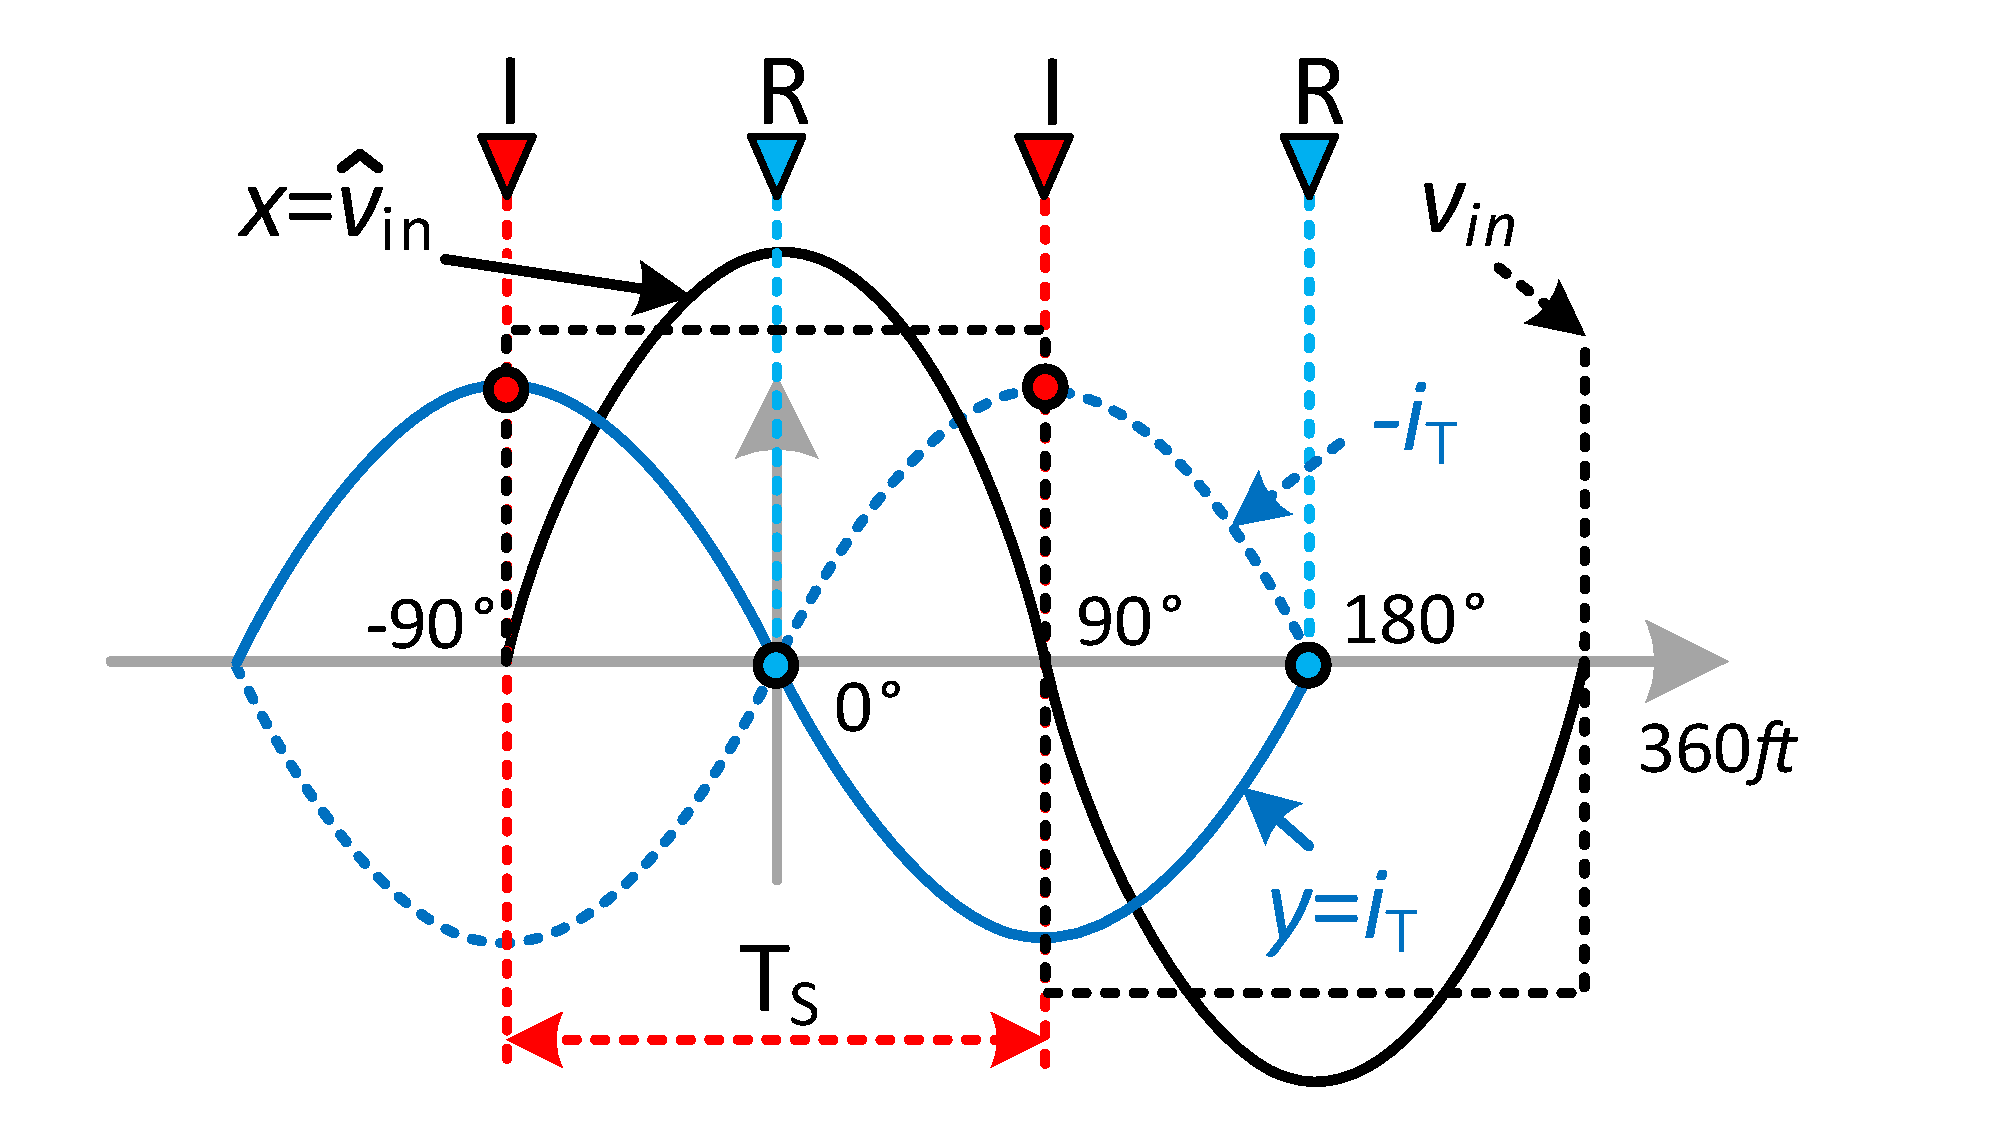
\includegraphics[clip, trim=-80mm 5mm -80mm 5mm, width=1\columnwidth]{FIGS/FIG12.pdf}
	     \caption{PWM-synchronized sampling with the reference of the input voltage PWM to take samples from the imaginary ``I" and real ``R" components of the output signal $i_\mathrm{T}$.}
	     \label{FIG12}
	     \vspace{0mm}
	 \end{figure}	  
	 
	 To implement the SOPWMS2, the dominant {\color{red}orientation} of the vertically shifted transfer function needs to be identified. This {\color{red}orientation} usually follows the steady-state behavior of the system ($\mathfrak{H}(0)$). However, when the suppression of the system transients is concerned, the effective frequency bandwidth of this {\color{red}orientation} should be determined. This step has been taken in Section III, and it has been shown that the given system in its effective band-width of operation ($0~\mathrm{Hz}$ to $5~\mathrm{kHz}$) is inclined towards its imaginary component (as shown in Fig~\ref{FIG9}), and its dominant orientation is $90^\circ$. Therefore, it has almost a constant phase angle of $90^\circ$ in its operating band-width, and its whole behavior can be estimated by taking PWM-synchronized samples from
	 ``I" instances shown in Fig.~\ref{FIG12}, where its sampling phase angle with the reference to its input variable ($v_\mathrm{in}$) is the same with the effective phase angle (dominant orientation) of its vertically shifted model $\angle \mathfrak{H}(0)$. Finally, the coefficients of the PI controller is tuned in such a way that it can effectively control the system and stabilize its transients with the use of the obtained PWM-sampled output signal $i_\mathrm{T}$. For this purpose, the Nyquist contours of the vertically shifted system $\mathfrak{H}(\mathrm{j}\omega)$ together with its real $\mathfrak{H}_\mathrm{R}(\mathrm{j}\omega)$ and imaginary $\mathrm{j}\mathfrak{H}_\mathrm{R}(\mathrm{j}\omega)$ parts are depicted in Fig.~\ref{FIG13}. Having all poles and zeros of $\mathfrak{H}(s)$ on the left-side of the s-plane, the minimum stability margins of these systems, with the specifications given in Table~\ref{TBL1}, are {\color{red}$\mathrm{PM}(\mathfrak{H}(\mathrm{j}\omega))=63.6^\circ$,} $\mathrm{GM}(\mathfrak{H}(\mathrm{j}\omega))=-18.25~\mathrm{dB}$, $\mathrm{PM}(\mathfrak{H}_\mathrm{R}(\mathrm{j}\omega))=16.1^\circ$, $\mathrm{GM}(\mathfrak{H}_\mathrm{R}(\mathrm{j}\omega))=-4.39 ~\mathrm{dB}$, $\mathrm{PM}(\mathfrak{H}_\mathrm{I}(\mathrm{j}\omega))=12.8^\circ$, $\mathrm{GM}(\mathfrak{H}_\mathrm{I}(\mathrm{j}\omega))=-5.81~ \mathrm{dB}$.
	 
	 %% FIG13
	 \begin{figure}
	     \centering
	     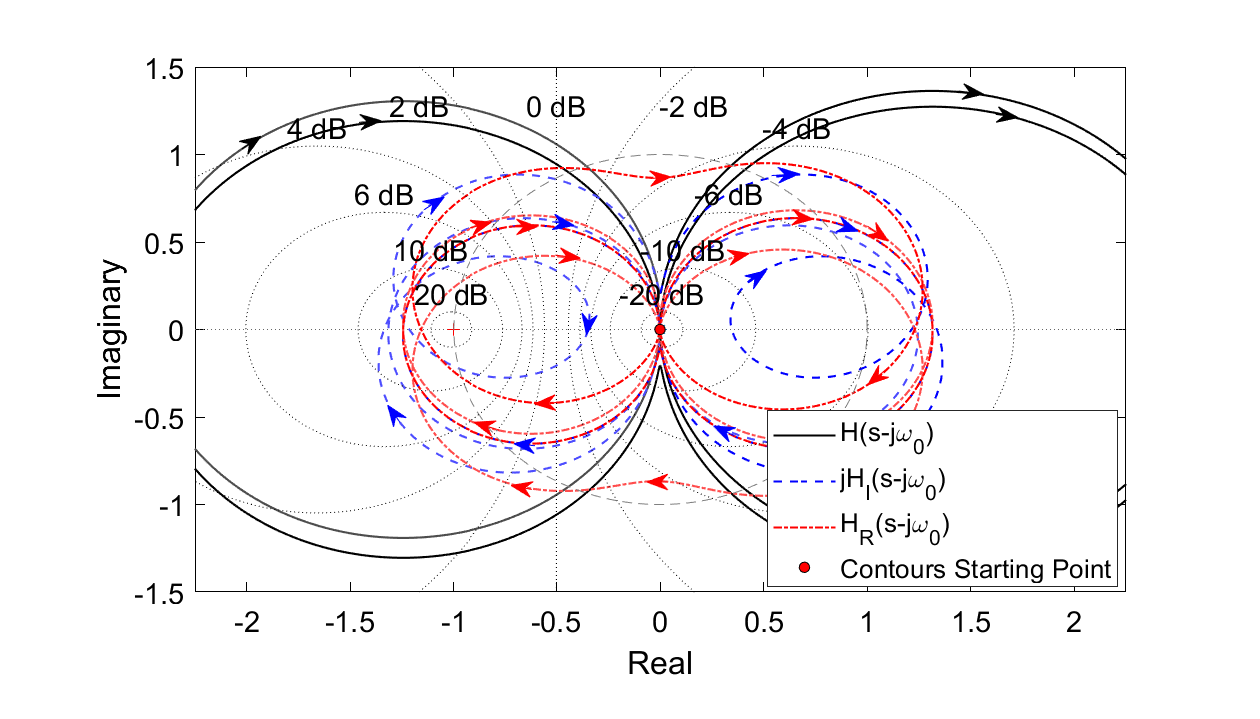
\includegraphics[clip, trim=1cm 0cm 1cm 0cm, width=1\columnwidth]{FIGS/FIG13.eps}
	     \caption{Nyquist contours of the vertically shifted transfer function $\mathfrak{H}(s)$, and its real $\mathfrak{H}_\mathrm{R}(s)$ and imaginary $\mathrm{j}\mathfrak{H}_\mathrm{I}(s)$ parts (the contours of $\omega~<~0$ are depicted in a lighter color and the starting point of $\omega \rightarrow -\infty$ is shown by a red circular marker).}
	     \label{FIG13}
	     \vspace{-3mm}
	 \end{figure}
	 
	 These margins show that without the involvement of any controller, the system closed-loop transfer function is unstable. It can also be seen that the imaginary transfer function $\mathrm{j}\mathfrak{H}_\mathrm{I}(s)$ is closer to unsuitability region than the real part $\mathfrak{H}_\mathrm{R}(s)$. Therefore, these margins partially show that the imaginary transfer function is more sensitive against the input changes than the real part, and in comparison to the real part, the imaginary part can be chosen for the feedback loop to stabilize the dynamics of the system as it contains more system information.
	 
	 The following shows the way by which samples are taken from $Y_\mathrm{I}(s)$ (obtained from $\mathfrak{H}_\mathrm{I}(s)$), and they are fed back to the close loop discrete controller so that the system can be stabilized. By taking samples from the quadrature component of the transmitter current $i_\mathrm{T}(t)$, the sampler observes only the imaginary part of the vertically shifted transfer function ($\mathfrak{H}_\mathrm{I}(s)$). Hence, for the proposed technique of sampling, the generic closed-loop block diagram of the system shown in Fig.~\ref{FIG11} is reconfigured to what is shown in Fig.~\ref{FIG14}(a), which can be further simplified into Fig.~\ref{FIG14}(b).
	 
	 %% FIG14
	 \begin{figure}
	    \begin{center}
	        \subfloat[]{
	                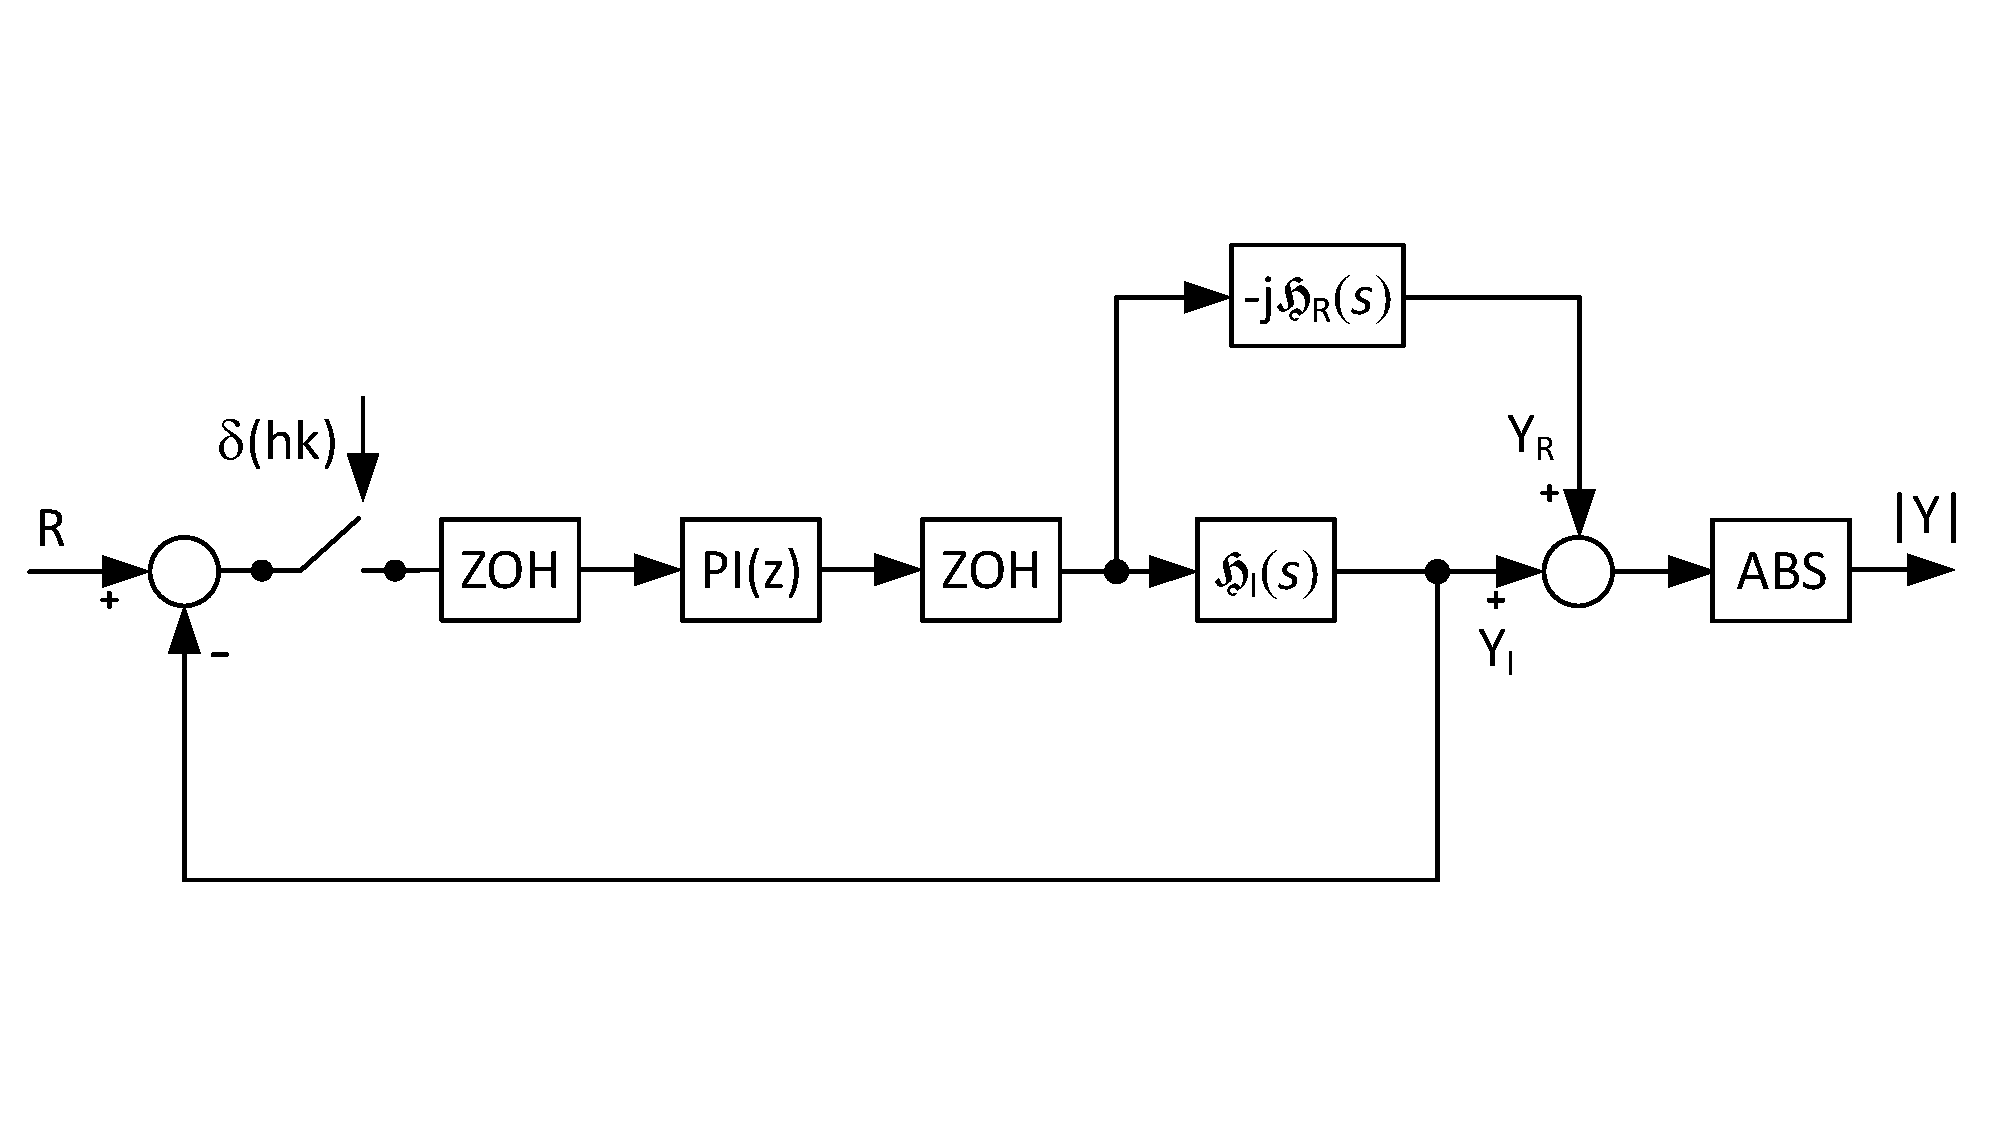
\includegraphics[clip, trim=-5mm 40mm -5mm 40mm, width=1\columnwidth]{FIGS/FIG14A.pdf}
	                }\\
	                \vspace{-3mm}
	        \subfloat[]{
	                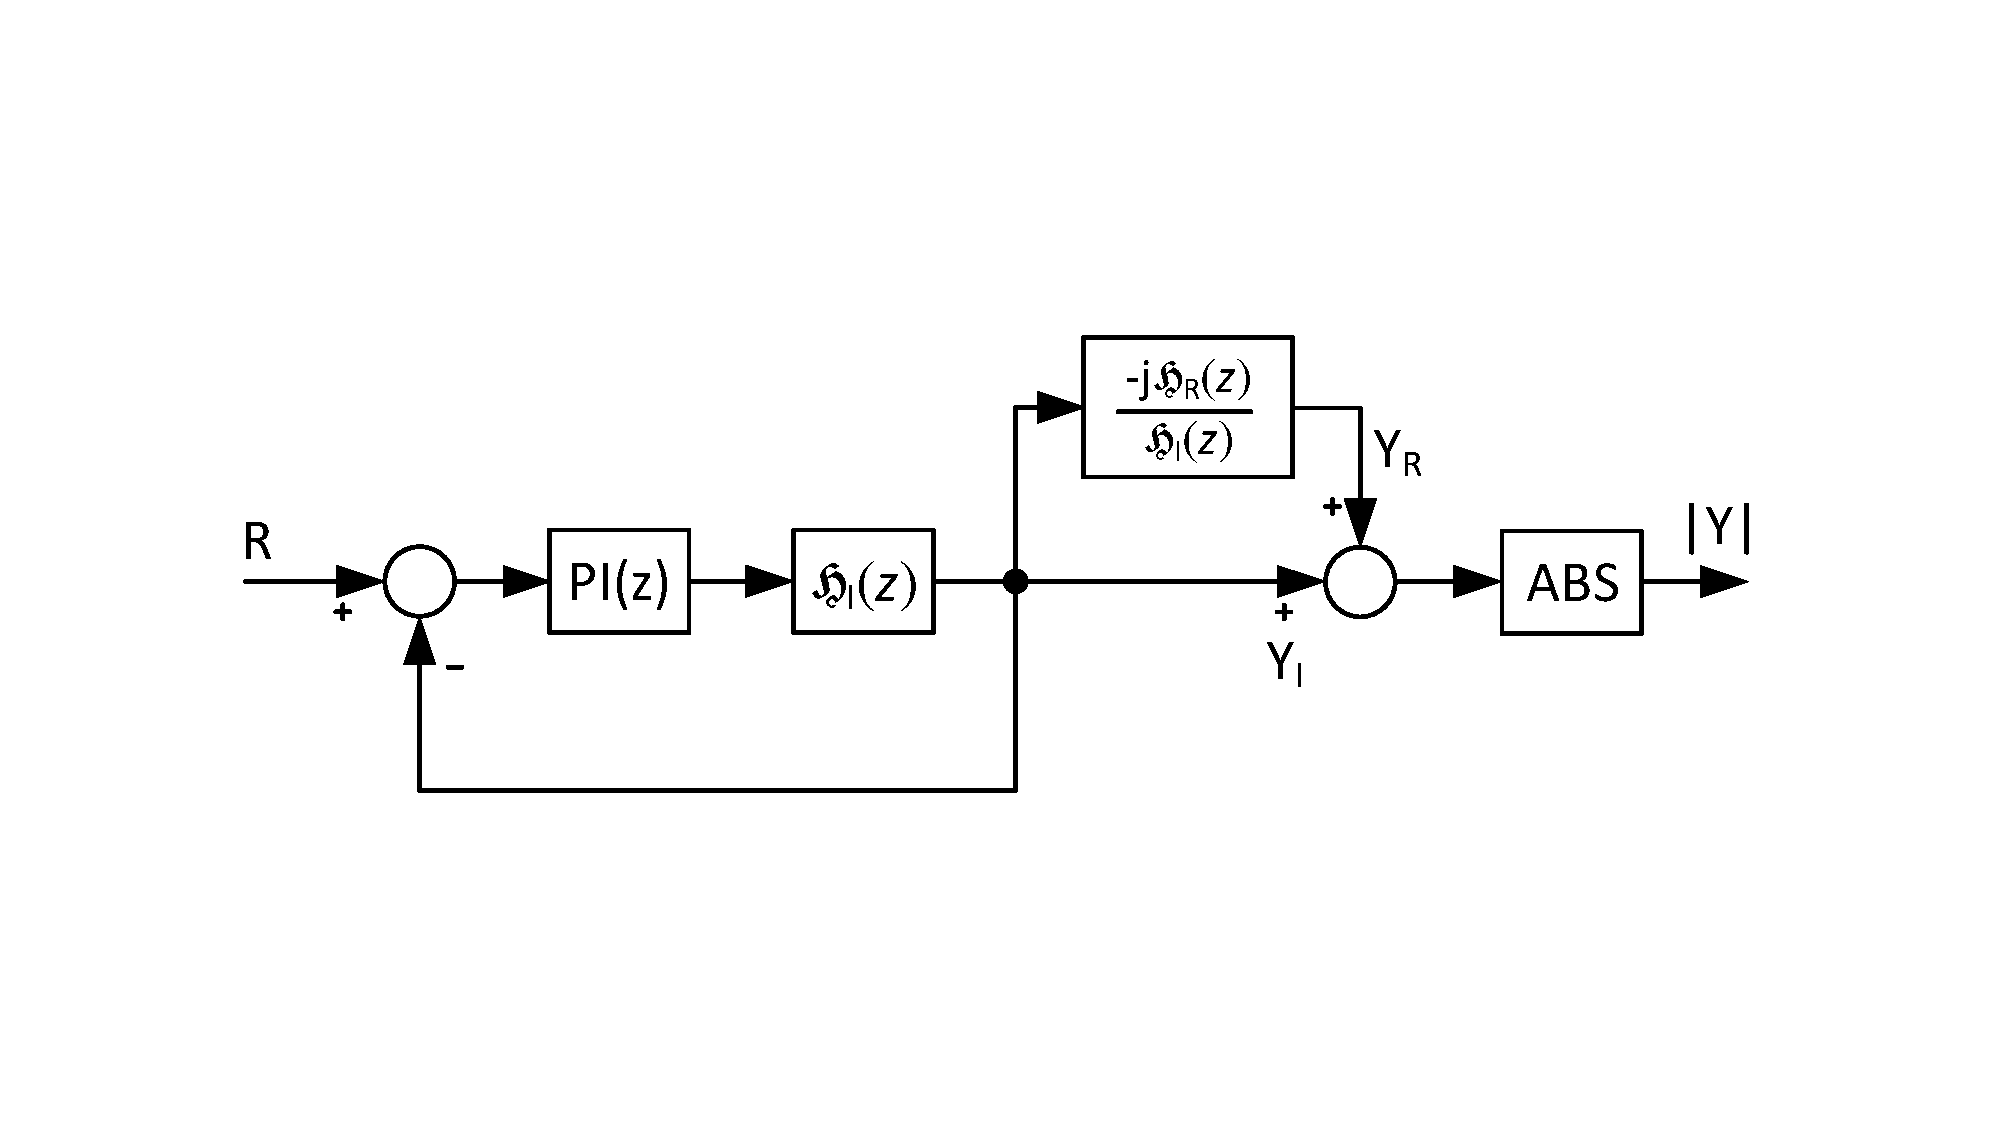
\includegraphics[clip, trim=-5mm 50mm -5mm 50mm, width=1\columnwidth]{FIGS/FIG14B.pdf}
	                }
	    \end{center}
	    \vspace{-3mm}
	    \caption{Reconfigured block diagram of the feedback loop for $\mathfrak{H}(s)$ shown in Fig.~\ref{FIG11}; (a) Imaginary sampled system consisting of $\mathfrak{H}_\mathrm{I}(z)$ loop transfer function, which can be simplified into the block diagram shown in (b).}
	    \label{FIG14}
	    \vspace{-3mm}
	\end{figure}
	 
	 
	 To achieve a desirable stability for the obtained system shown in Fig.~\ref{FIG14}(b), the discrete domain loop transfer function of $\mathrm{PI}(z)\mathfrak{H}_\mathrm{I}(z)$ needs to meet the required stability margins, and $\mathfrak{H}_\mathrm{I}(z)$ should possess stable zeros. {\color{red}In the proposed approach, the highest achievable sampling interval for the given system is $T_\mathrm{S}=\pi/\omega_0$.} For this sampling rate, discrete domain poles and zeros of $\mathfrak{H}_\mathrm{I}(z)$ are depicted in Fig. \ref{FIG15} which show that sampled plant has stable zeros and poles. Therefore, $-\mathrm{j}{\mathfrak{H}_\mathrm{R}(z)}/{\mathfrak{H}_\mathrm{I}(z)}$ branch of the sampled control system shown in Fig.~\ref{FIG14}(b) is stable.
	 
	 %% FIG15
	 \begin{figure}
	     \centering
	     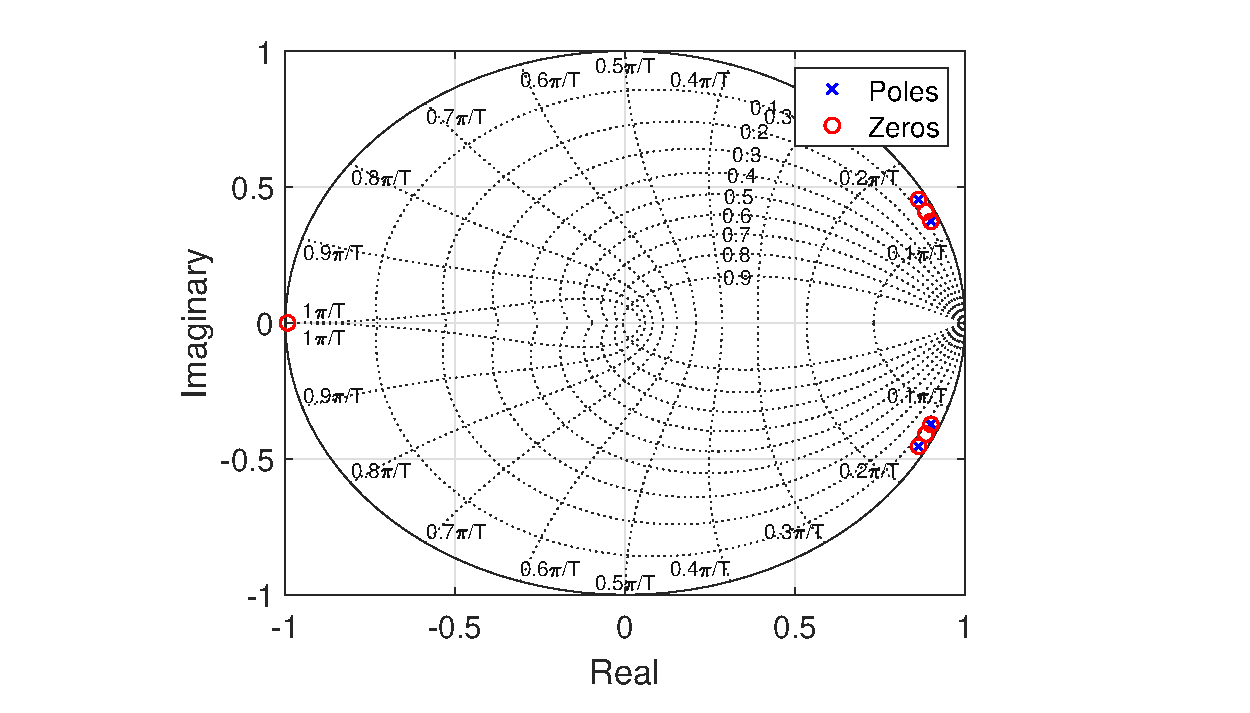
\includegraphics[clip, trim=0.7cm 0cm 1cm 0cm, width=1\columnwidth]{FIGS/FIG15.eps}
	     \caption{Poles and zeros of the sampled plant $\mathfrak{H}_\mathrm{I}(z)$ for the sampling interval of $T_\mathrm{S}=2\pi/\omega_0$.}
	     \label{FIG15}
	     \vspace{-3mm}
	 \end{figure}
	 
	 Having the sampling interval of $T_\mathrm{S}=2\pi/\omega_0$, in the next step, the discrete domain PI controller coefficients are tuned to achieve desirable stability margins. This is done with the use of Nyquist diagram obtained from the sampled system shown in Fig.~\ref{FIG16}. In this diagram, the solid blue line is related to the stable closed-loop which is obtained by setting $K_\mathrm{p}=0.2$ and $K_\mathrm{i}=40\mathrm{k}$. The corresponding stability margins for the stable closed-loop are $\mathrm{PM}(\mathrm{PI}(z)\mathfrak{H}_\mathrm{I}(z))=89.3^\circ$ and $\mathrm{GM}(\mathrm{PI}(z)\mathfrak{H}_\mathrm{I}(z))=7.49~\mathrm{dB}$.
	 %Under other conditions, for $K_\mathrm{p}=0.5$ and $K_\mathrm{i}=100~\mathrm{k}$, the open-loop transfer function would be unstable as depicted in the solid red line.

	 %% FIG16
	 \begin{figure}
	     \centering
	     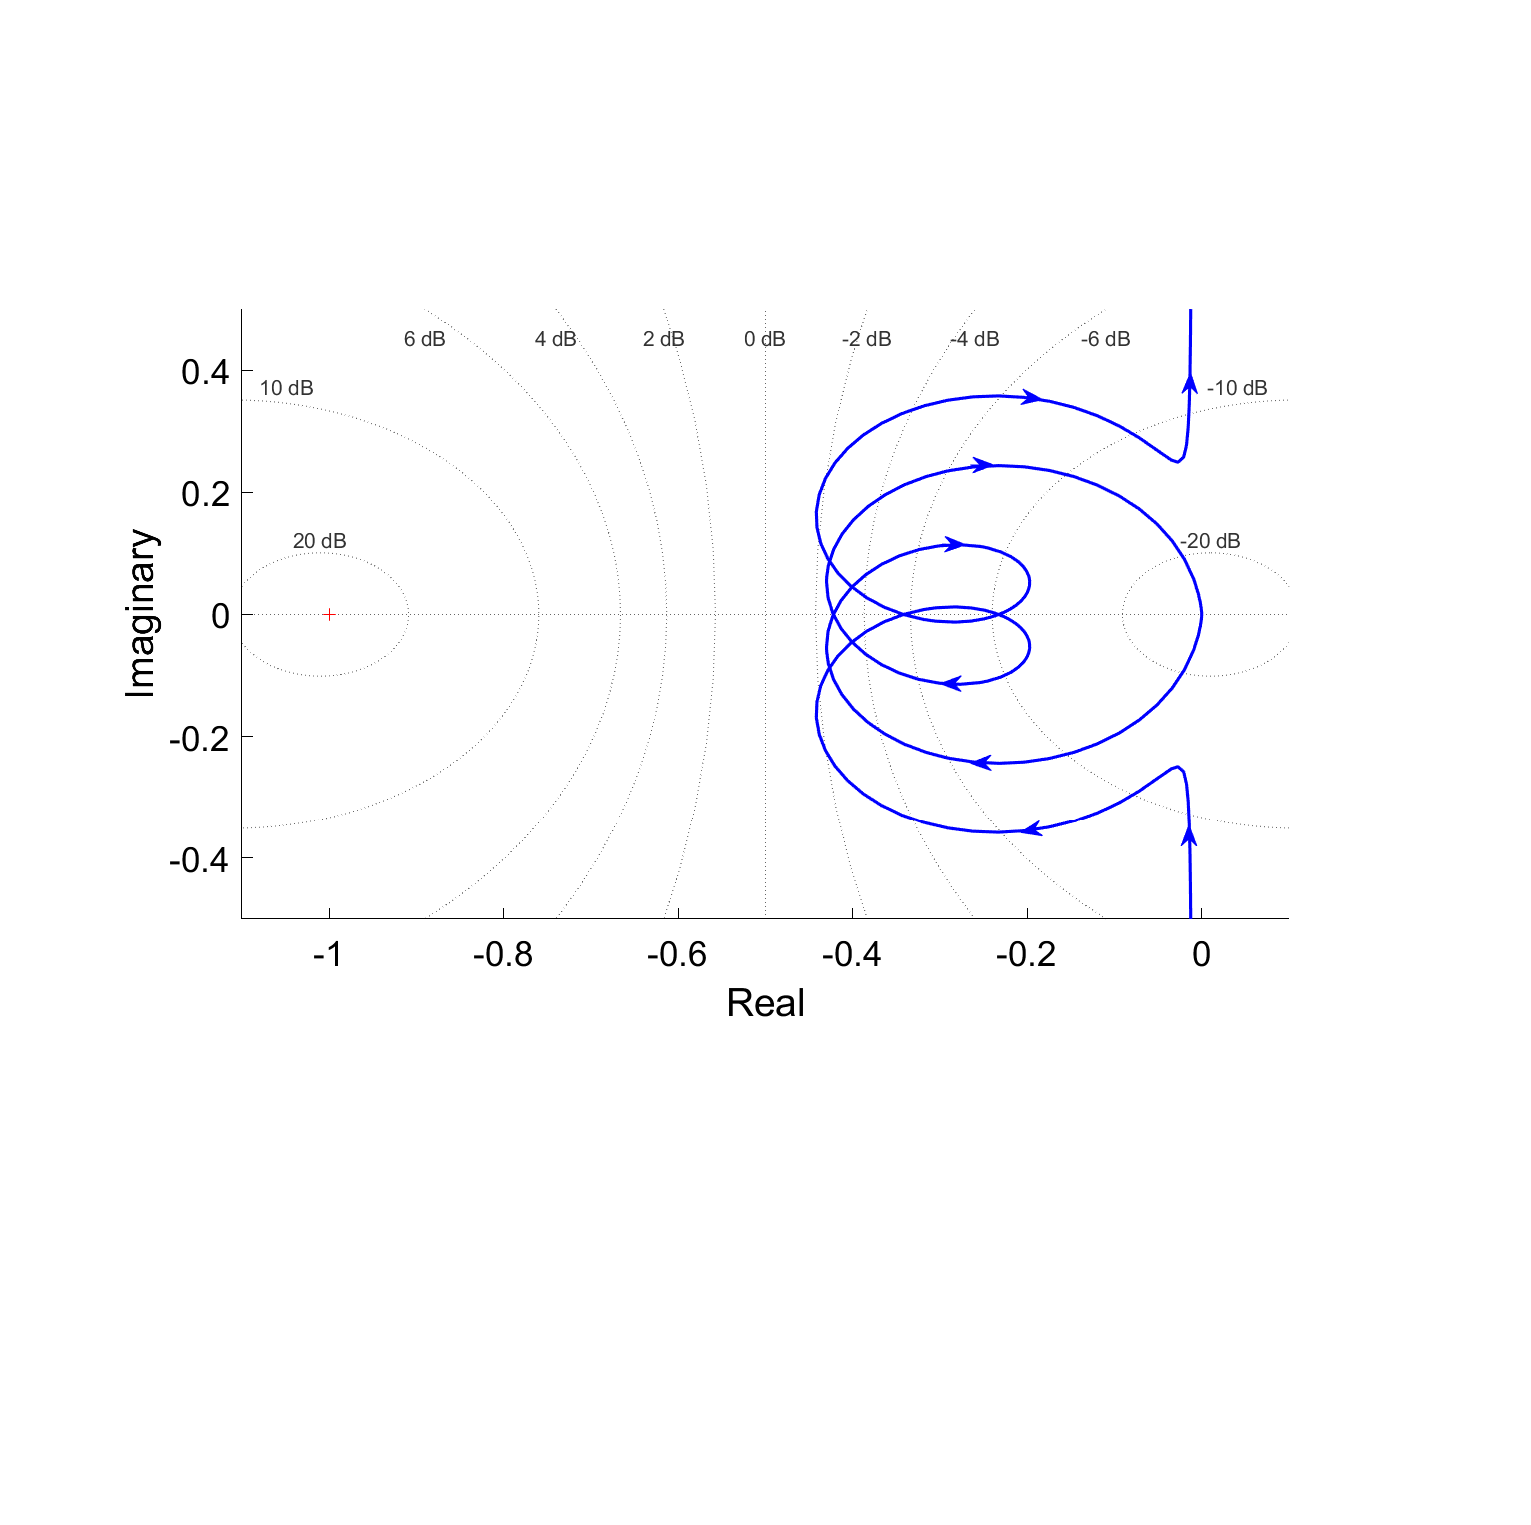
\includegraphics[clip, trim=1.75cm 8.25cm 2.75cm 4cm, width=1\columnwidth]{FIGS/FIG16.eps}
	     \caption{Nyquist diagrams of the stable (solid-blue line) open-loop discrete domain transfer function $\mathrm{PI}(z)\mathfrak{H}_\mathrm{I}(z)$.}
	     \label{FIG16}
	     \vspace{-3mm}
	 \end{figure}
	 
	 To show that by taking samples from the imaginary contents of the output signal is sufficient to make the proposed system stable, the system shown in Fig.~\ref{FIG2} is simulated based on the specifications given in Table I and for the obtained coefficients for $K_\mathrm{p}$ and $K_\mathrm{i}$. The response of $i_\mathrm{T}$ after applying a step change of amplitude (reference signal) is shown in Fig.~\ref{FIG17}. In the simulations, the detailed models of the H-Bridge converter and LCC network are included, and to have a higher time resolution for the sampled system, the input signal of $i_\mathrm{T}$ is rectified and sampled at the moments of input voltage $v_\mathrm{in}$ zero crossings where $i_\mathrm{T}$ can reveal its quadrature component. The obtained envelope signal is fed to the PI controller and by properly tuning the gain of the duty ratio, the controller can generate the desired phase angle $\phi$ {\color{red}between the PWMs of the inverter legs} so that the transmitter current $i_\mathrm{T}$ follows its set point ($I_\mathrm{T,ref}$).
	 
	 %% FIG17
	 \begin{figure}
	 \vspace{0.4cm}
	     \centering
	     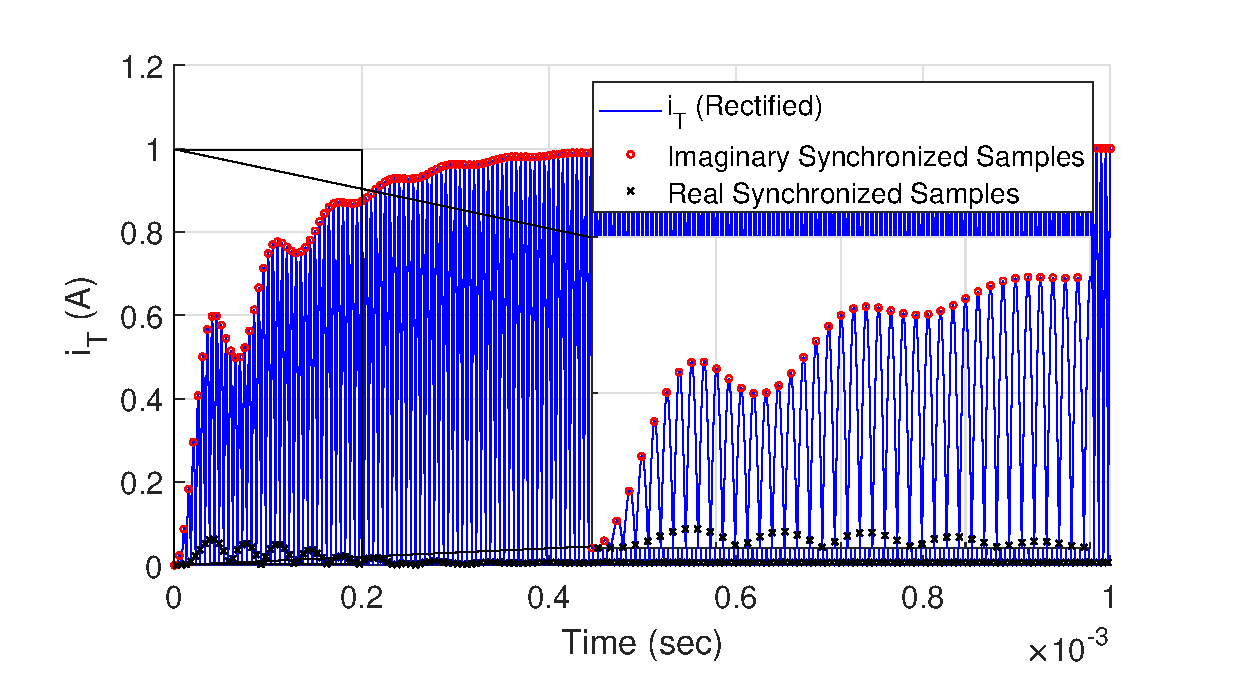
\includegraphics[clip, trim=0.7cm 0cm 1cm 0cm, width=1\columnwidth]{FIGS/FIG17.eps}
	     \caption{Time-domain strictly proper $i_\mathrm{T}$ signal obtained from the simulated system shown in Fig.~\ref{FIG2}. Blue line shows the rectified transmitter current, red circular markers show the imaginary PWM-synchronized samples, and black crossed markers show the real PWM-synchronized samples.}
	     \label{FIG17}
	     \vspace{-3mm}
	 \end{figure}
	 
	  %% I AM HERE
	 Worthy to mention that as the proposed technique of SOPWMS2 relies on ZOH sampling, its discrete domain poles and zeros are changed when the sampling interval changes. As such, unlike the continuous domain system transfer function, dynamic behavior of the system in discrete domain can be influenced by the sampling rate. %Although the stability of continuous domain poles is enough to make sure all the discrete domain poles are stable, the expansion of discrete domain zeros strictly rely on the sampling rate. 
	 In other words, a stable continuous domain system with all zeros and poles on the left-half of the s-plane (minimum-phase system) is not necessarily stable in discrete domain \cite{UNSTABLE_1,UNSTABLE_2}.
	 
	 Therefore, the influence of change in sampling interval on the sampled system stability is studied below. It is worth of mentioning that, in this work, to increase the rate of information, the transmitter current is rectified ($i_\mathrm{T}$), and the samples are taken per each half-cycle of the input voltage fundamental. Therefore, in this work, the sampling interval is set to $T_{\mathrm{S}0}=\pi/\omega_0=5~\mathrm{\mu s}$. 
	 To start with, discrete domain poles and zeros of the open-loop sampled system ($\mathrm{PI}(z)\mathfrak{H}_\mathrm{I}(z)$) are derived for different sampling intervals. For clarity, $h$ is defined as the ratio of the sampling period $T_\mathrm{S}$ to the minimum feasible period of sampling $T_{\mathrm{S}0}$ ($h={T_\mathrm{S}}/{T_{\mathrm{S}0}}$). 
	 %To realize the proposed approach of PWM-synchronized sampling {the sampling period needs to be an integer multiplex of the minimum feasible sampling period ($T_\mathrm{S0}$)}. 
	 To show how poles and zeros of the sampled system move on z-plane, they are calculated when sampling ratio $h$ changes from $0.1/T_\mathrm{S0}$ to $2/T_\mathrm{S0}$, and their displacement is shown in Fig.~\ref{FIG18}. This also gives some insights about the importance of discrete domain analysis for other sample-based approaches of envelope detection.
	 
	 %% FIG18
	 \begin{figure}
	     \centering
	     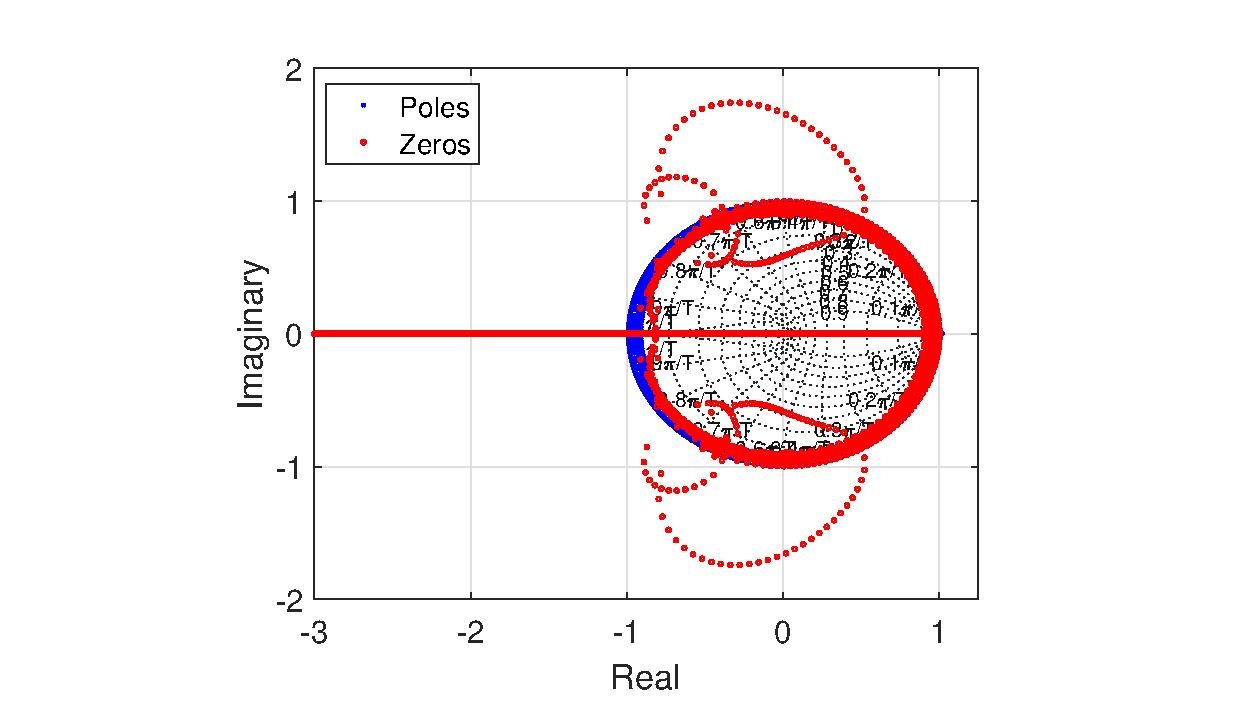
\includegraphics[clip, trim=1cm 0.1cm 1cm -0.1cm, width=1\columnwidth]{FIGS/FIG18.eps}
	     \caption{Discrete domain displacement of poles and zeros of the open-loop sampled system $\mathrm{PI}(z)\mathfrak{H}_i(z)$ when $h$ changes from $0.1h_0$ to $2h_0$.}
	     \label{FIG18}
	     \vspace{-3mm}
	 \end{figure}
	 
	 %% FIG19
	 \begin{figure}
	     \centering
	     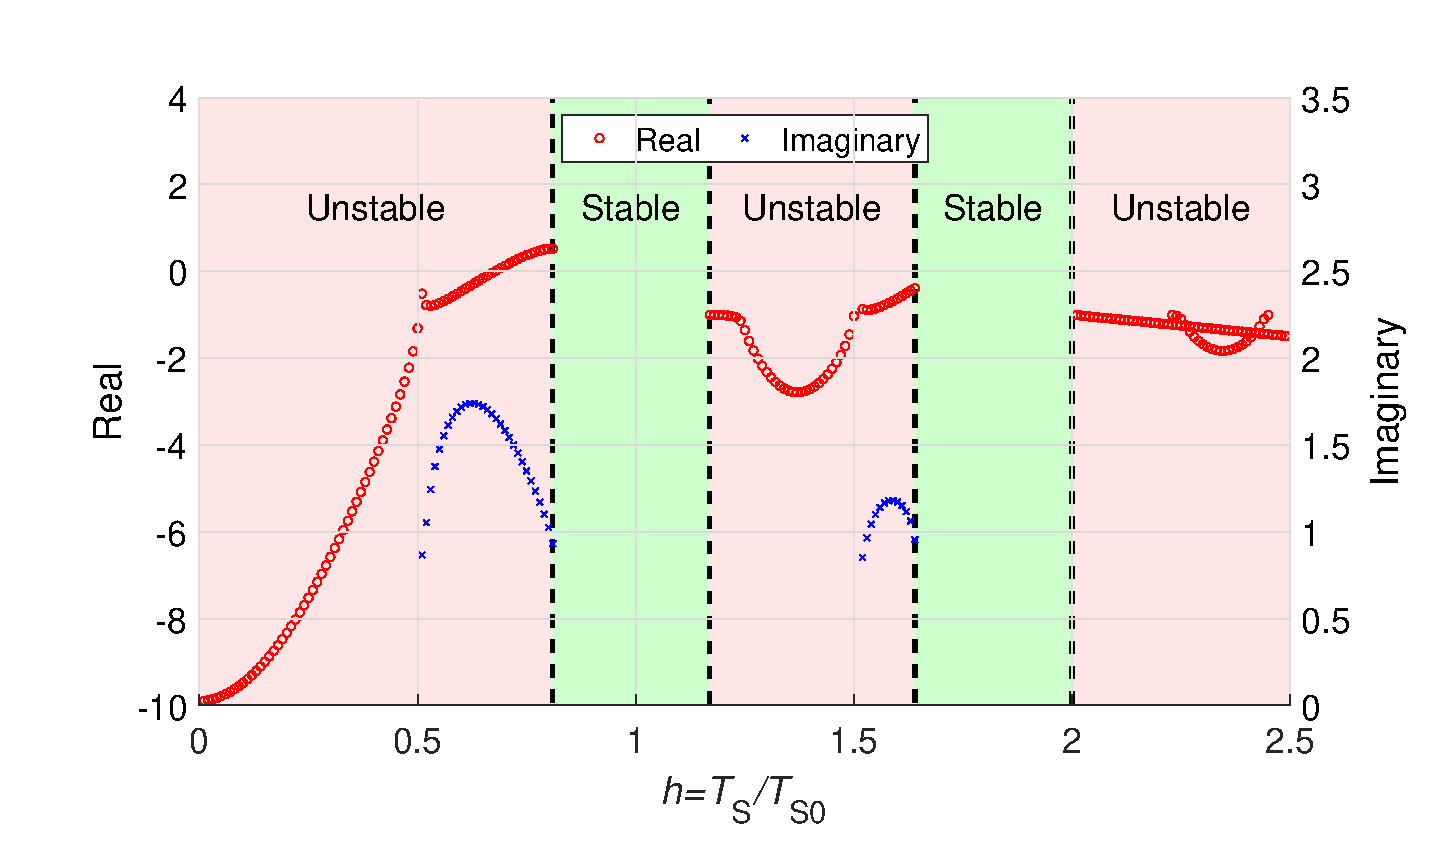
\includegraphics[clip, trim=1cm 0cm 0cm 0.4cm, width=1\columnwidth]{FIGS/FIG19.eps}
	     \caption{Discrete domain displacement of the unstable zeros in the sampled open-loop system $\mathrm{PI}(z)\mathfrak{H}_i(z)$ when $h$ changes from $0.1/T_\mathrm{S0}$ to $2/T_\mathrm{S0}$, red circular markers and blue crossed markers show the real and imaginary parts of the unstable zeros respectively.}
	     \label{FIG19}
	     \vspace{-3mm}
	 \end{figure}
	 
	 To have a better understanding of the influence of the sampling rate ($f_\mathrm{s}=1/T_\mathrm{S}$) on the open-loop {\color{red}unstable zero dynamics}, real and imaginary parts of these zeros are depicted in Fig.~\ref{FIG19}. This figure shows that there are certain rates of sampling at which some zeros of the open-loop transfer function move into the unstable regions. {\color{red}This figure also implies that for the feasible rate of sampling ($h=1$), there is a $20\%$ room for jittering for the synchronizing clock pulse. This tolerance against the clock pulse jittering, is less than $20\%$ when the rectified signal is directly fed to the controller, but still enough to effectively stabilize a real case scenario.} Referring to the fact that the poles and zeros of a discrete domain PI controller are located on the horizontal axis, the complex zeros belong to $\mathfrak{H}_\mathrm{I}(z)$ can lead to the instability of $-\mathrm{j}{\mathfrak{H}_\mathrm{R}(z)}/{\mathfrak{H}_\mathrm{I}(z)}$ and, consequently, the instability of the whole system. Hence, the necessity of studying the behavior of the sampled-system in different sampling rates is clear.
	 
	 As it can be seen in Fig.\ref{FIG17}, after implementing the proposed sampling technique and properly tuning the PI controller, the system can be effectively stabilized only by taking samples from the quadrature term of the transmitter current $i_\mathrm{T}$. 
	 %% HAVE A LOOK AT ME
	 %{\color{red} It is worthy to mention that as the stability with the use of SOPWMS2 is the major concern of this work, the effect of different controllers on the dynamic behavior of this paper is left to be done in future works.}
	 In the next section, the experimental results obtained from the WPT system are presented.
	 
	 
	 %In this  $\mathfrak{H}_\mathrm{I}(s)$ and $\mathfrak{H}_\mathrm{R}(s)$
	 
	 
	 \section{Experimental Results}
	 To prove the validity of the SOPWMS2 technique, the WPT system under study is experimentally built as shown in Fig.~\ref{FIG20}, and its specifications are given in Table~\ref{TBL1}.
	 {\color{red}The experimental scenario is designed such that the stability of the system is maintained, and the reference signal in the proposed system is tracked properly.}
	  %% FIG20
	 \begin{figure}
	    \begin{center}
	        \subfloat[]{
	                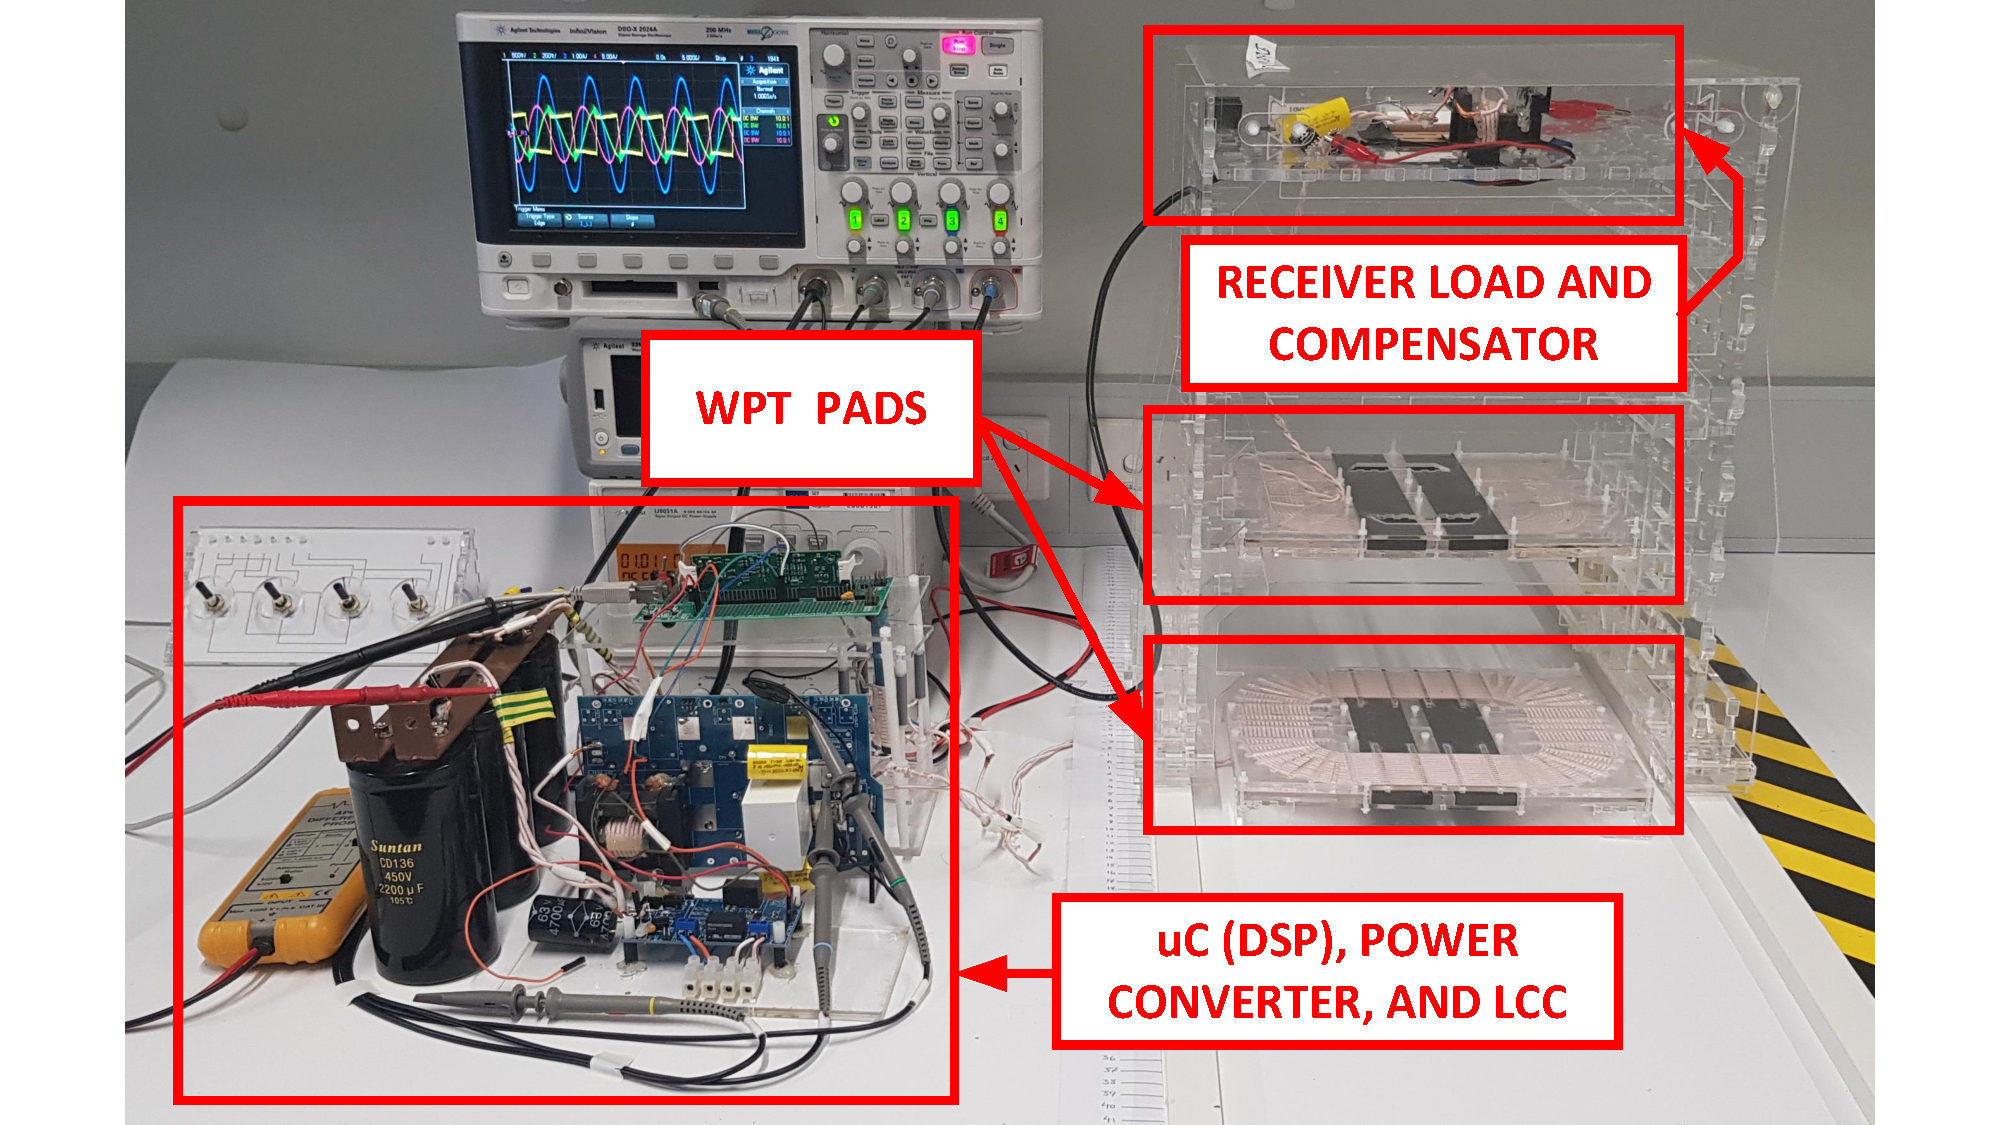
\includegraphics[clip, trim=20mm 0mm 20mm 0mm, width=1\columnwidth]{FIGS/FIG18A.pdf}
	                }\\
	                \vspace{-3mm}
	        \subfloat[]{
	                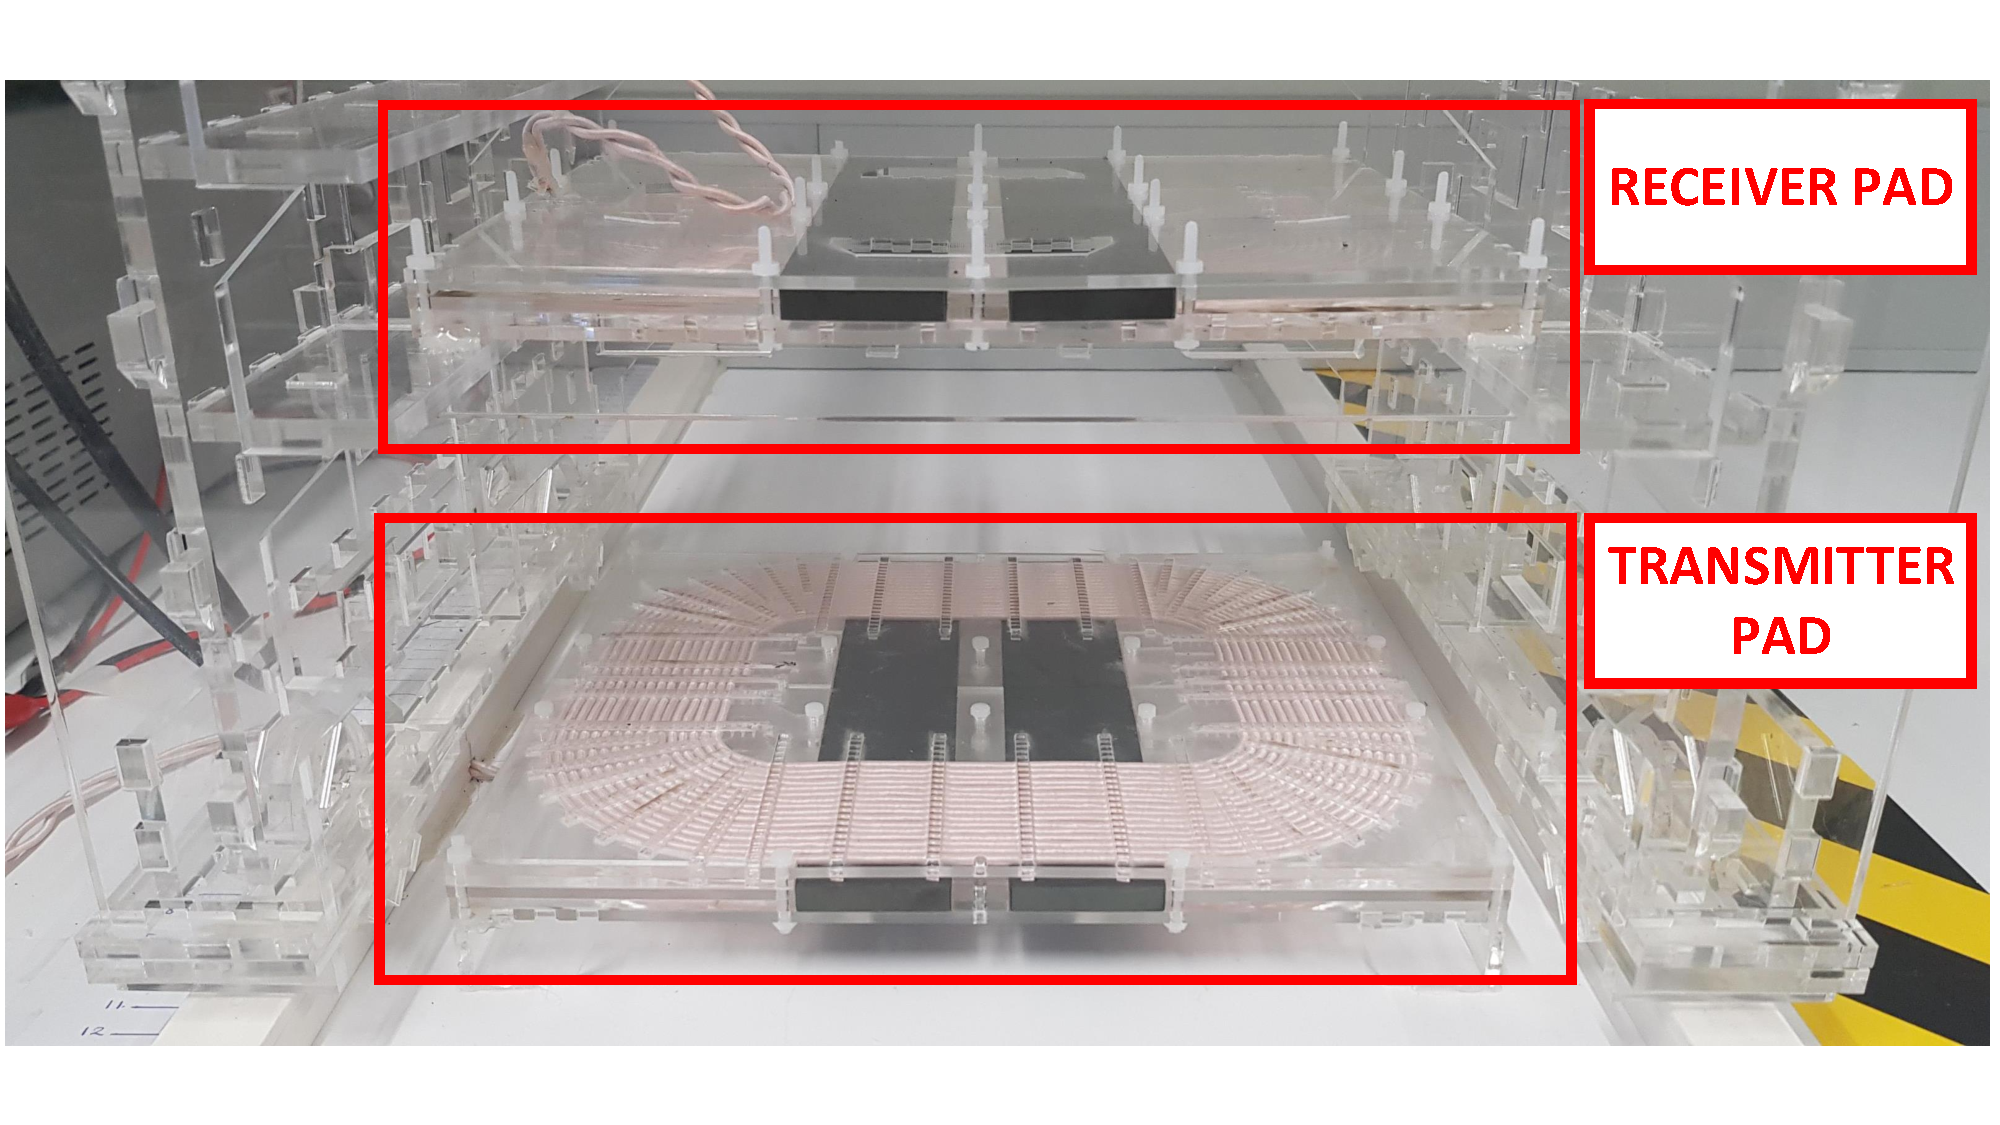
\includegraphics[clip, trim=0mm 10mm 0mm 10mm, width=1\columnwidth]{FIGS/FIG18B.pdf}
	                }\\
	                \vspace{-3mm}
	        \subfloat[]{
	                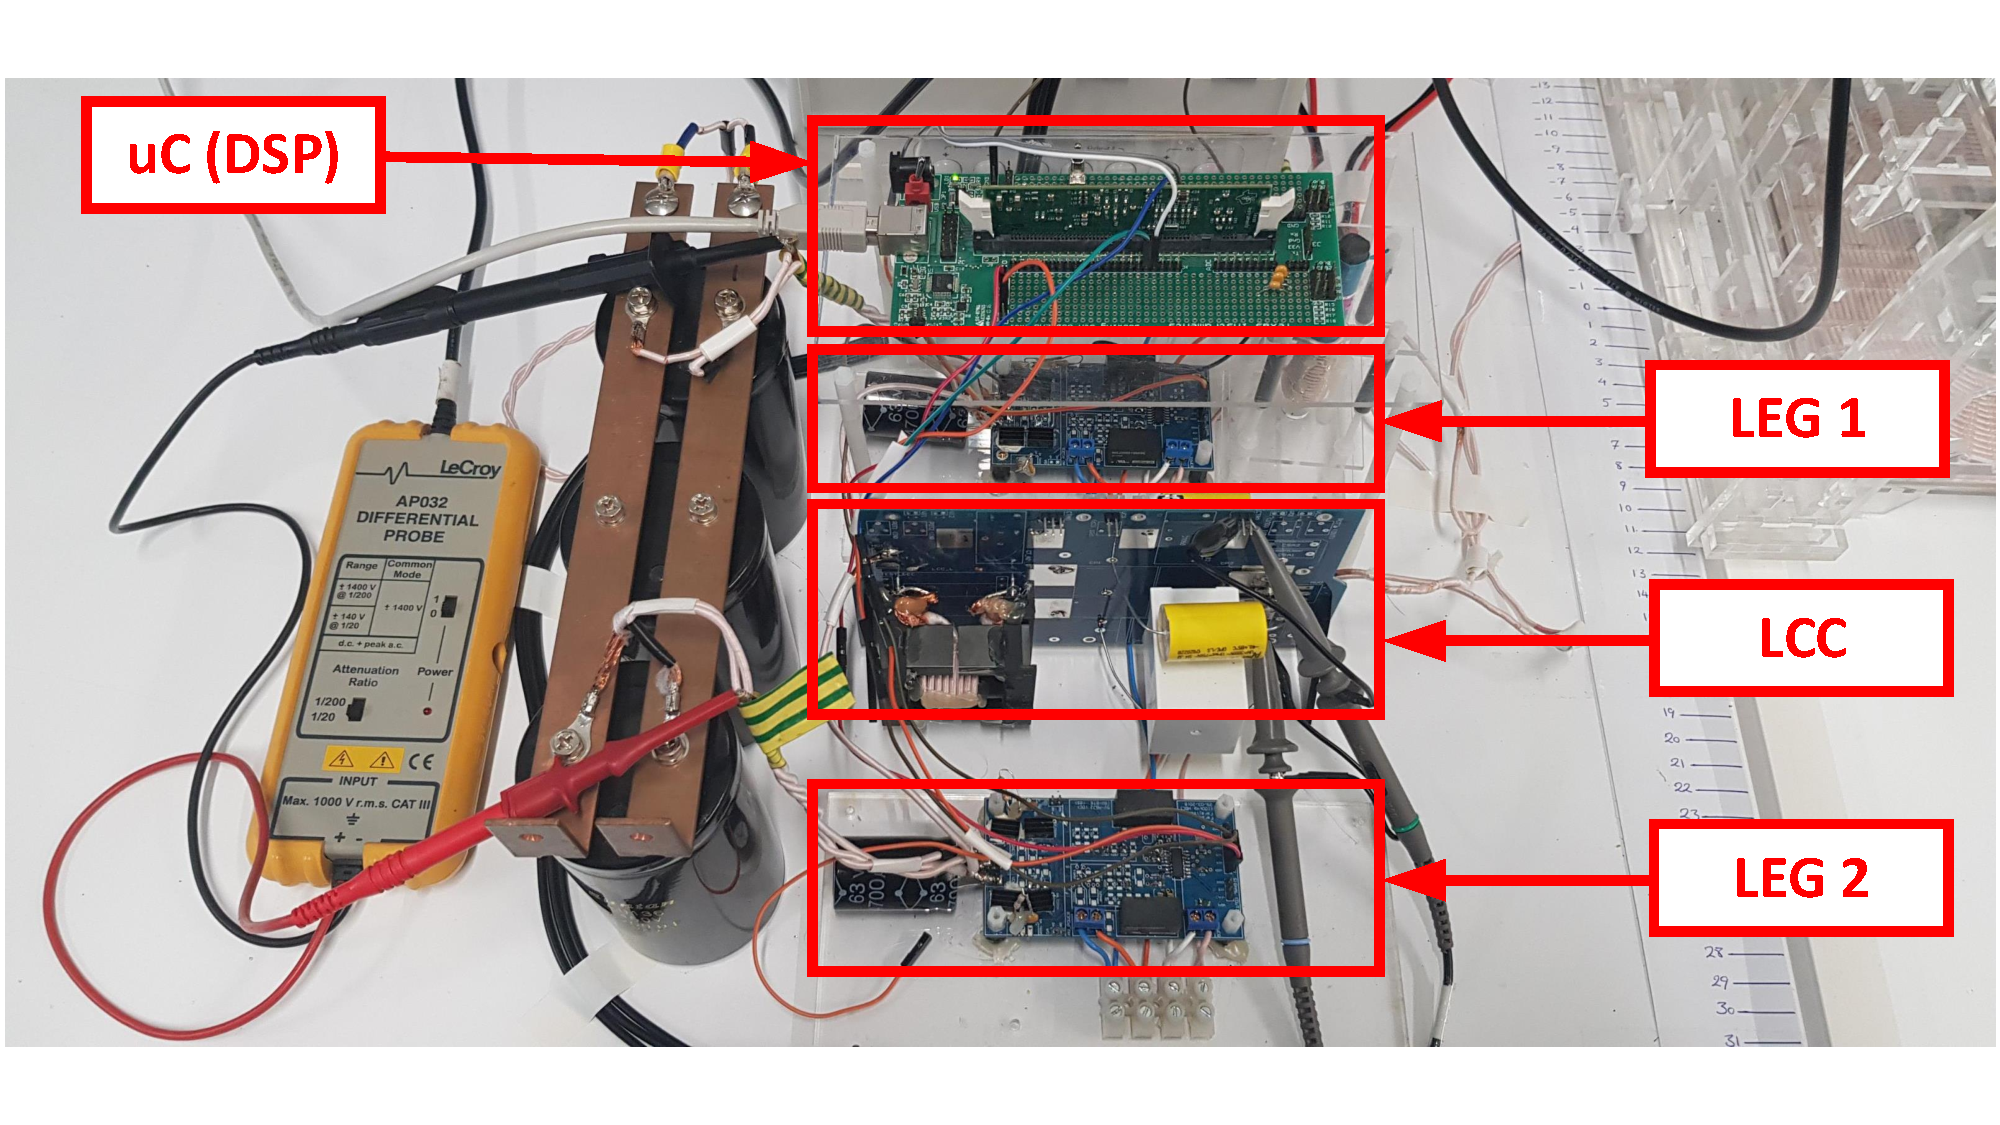
\includegraphics[clip, trim=0mm 10mm 0mm 10mm, width=1\columnwidth]{FIGS/FIG18C.pdf}
	                }
	    \end{center}
	    \vspace{-3mm}
	    \caption{The experimental setup; (a) whole the setup, (b) WPT pads, and (c) transmitter driving system.}
	    \label{FIG20}
	    \vspace{-3mm}
	\end{figure}
	 
	 %% TBL1
	 \begin{table} [b]
	    \begin{center}
	    \caption{Simulated and experimental specifications of the WPT system.}
	    \label{TBL1}
	            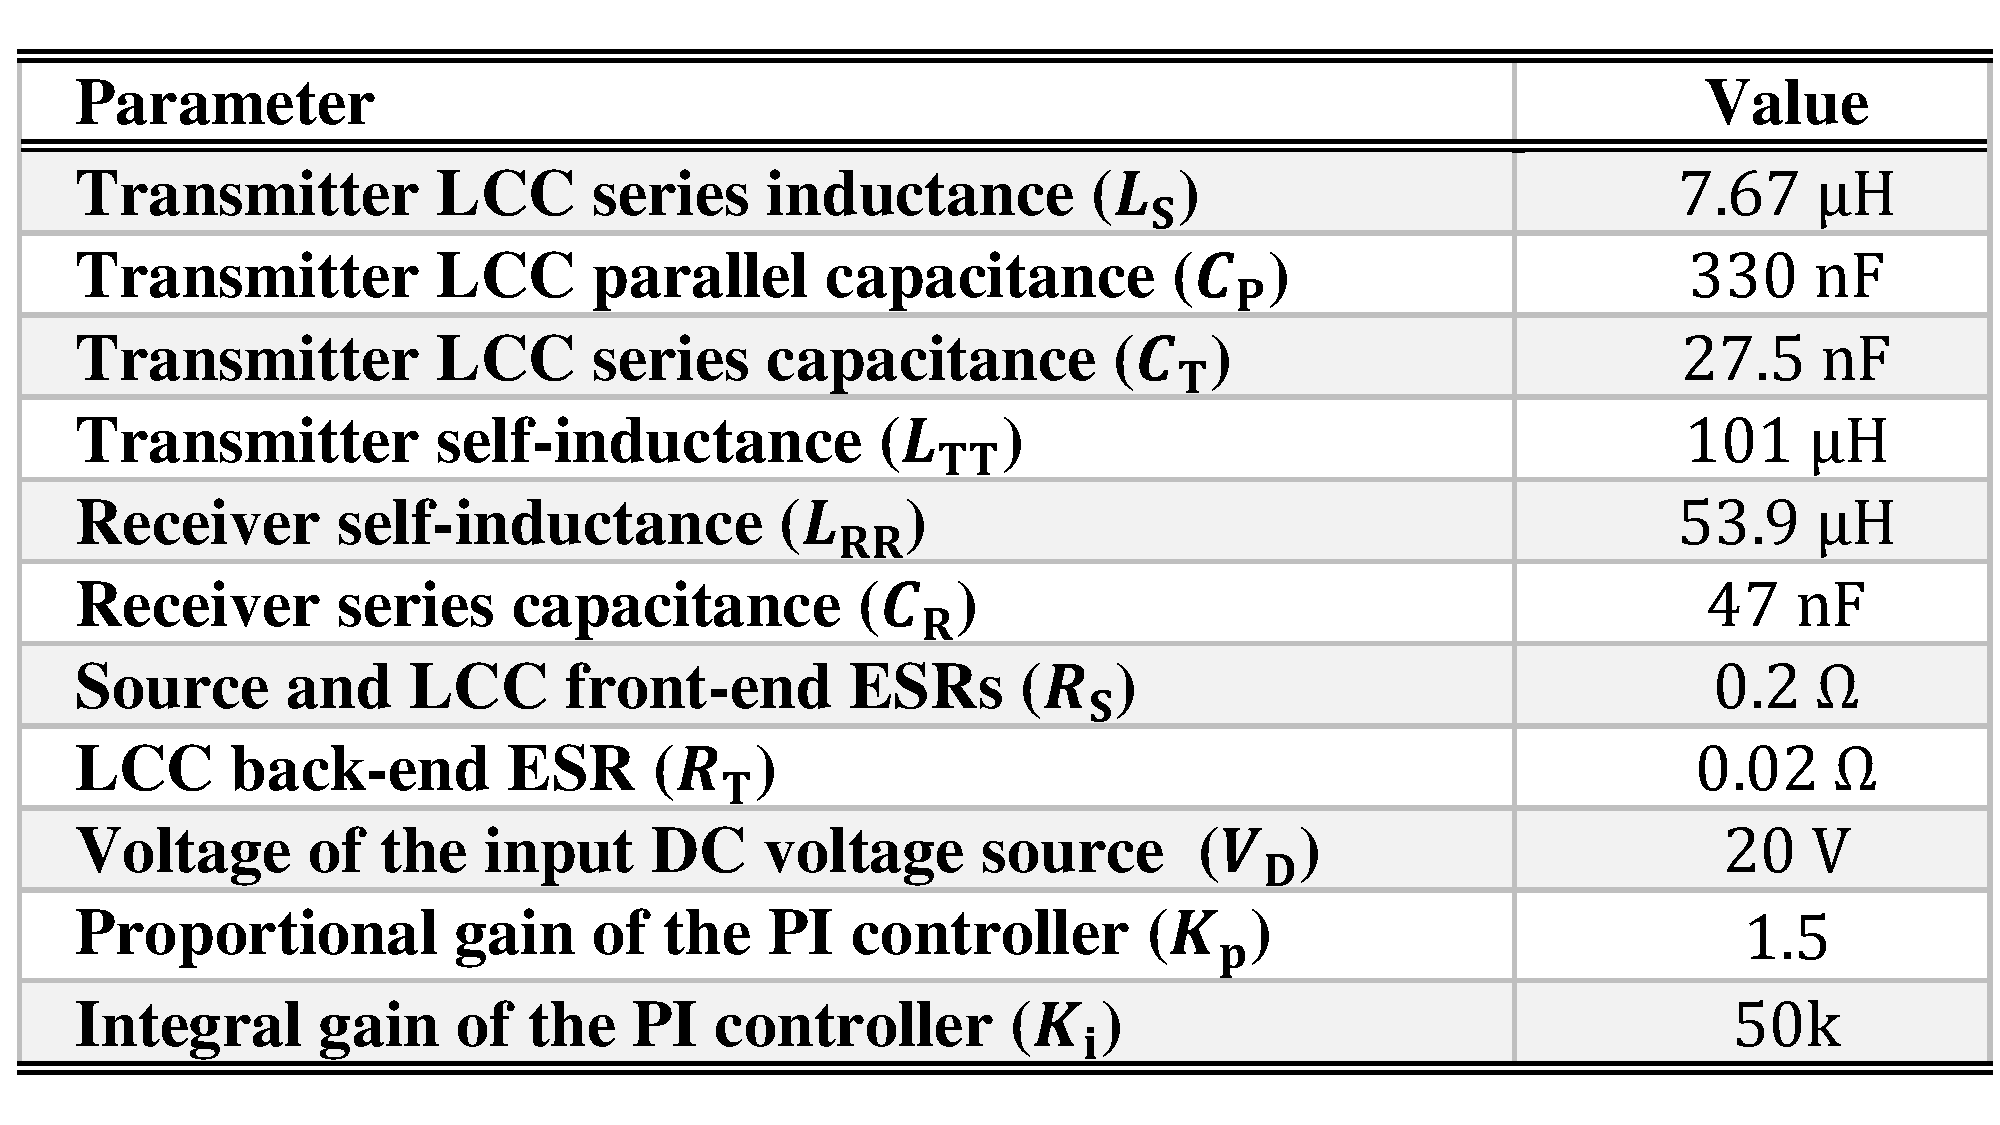
\includegraphics[clip, trim=0mm 10mm 0mm 10mm, width=1\columnwidth]{FIGS/TBL1.pdf}
	    \end{center}
	    \vspace{-3mm}
	\end{table}
	 
	 %In the first experiment a full-scale step of input voltage $V_{\mathrm{in}}$ ($0\%$ to $100\%$ is applied to the system without and with the presence of receiver. The results of this experiment is shown in Figs.~\ref{FIG21}(a) and (b) respectively.
	 In these experiments, step changes in the transmitter reference current $i_{\mathrm{T,ref}}$ for the cases of 0 A to 2 A and 1 A to 2 A for loaded and unloaded conditions are applied and the system responses are investigated.
	 
	 %% FIG21
	 \begin{figure}
	    \begin{center}
	        \subfloat[]{
	                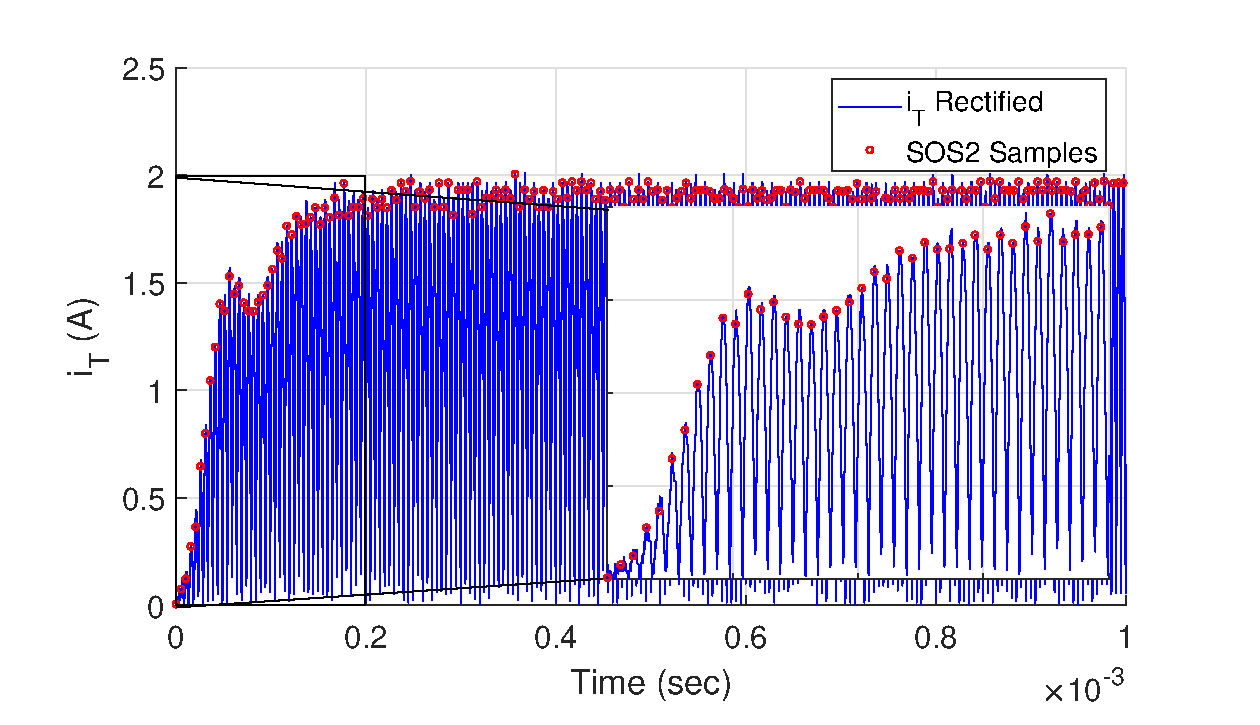
\includegraphics[clip, trim=0mm 1mm 0mm 6mm, width=1\columnwidth]{FIGS/FIG19A.eps}
	                }
	                \\
	                \vspace{-3mm}
	        \subfloat[]{
	                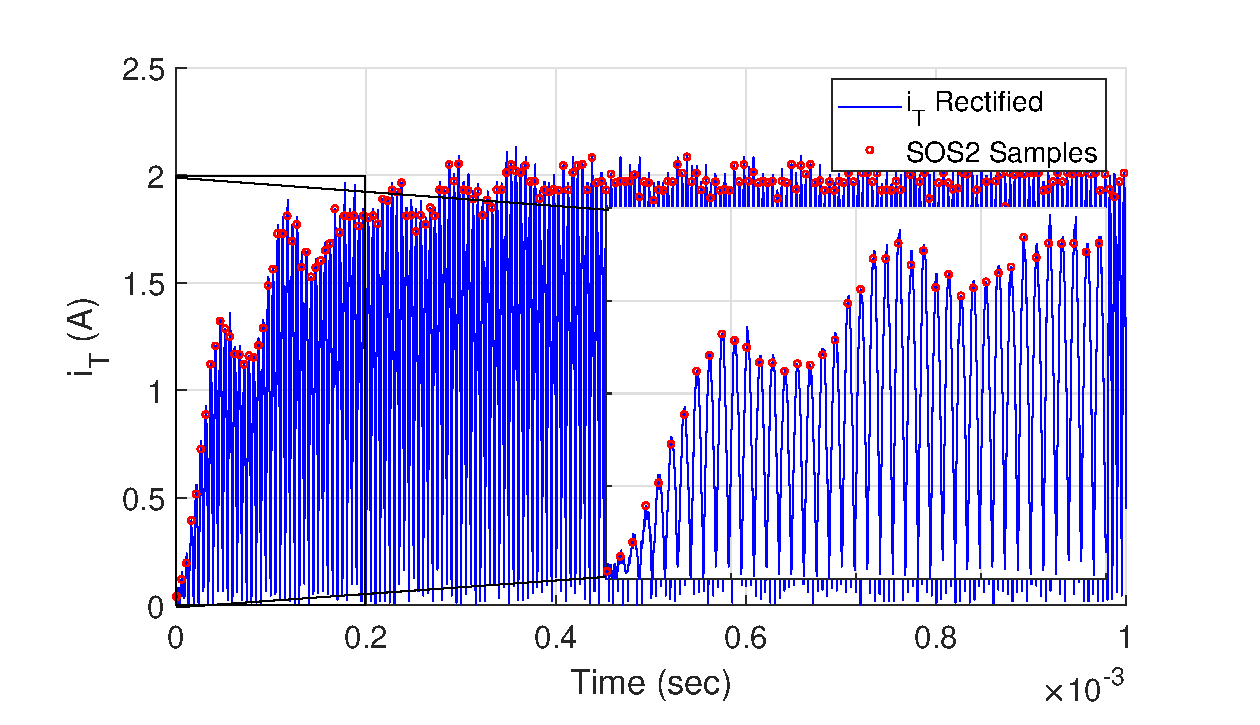
\includegraphics[clip, trim=0mm 1mm 0cm 6mm, width=1\columnwidth]{FIGS/FIG19B.eps}
	                }
	    \end{center}
	    \vspace{-3mm}
	    \caption{Experimental results for a full-scale change in the step change of input voltage for (a) no-load condition (no coupling between transmitter and receiver) and (b) loaded condition (transmitter and receiver interact).}
	    \label{FIG21}
	    \vspace{-3mm}
	\end{figure}
	 
	 For the first case of $i_{\mathrm{T,ref}}$ change from 0 A to 2 A, it can be seen in Fig.~\ref{FIG21}, the transmitter current $i_{\mathrm{T}}$ follows the input reference signal of $i_\mathrm{T,ref}$ effectively. The single-oriented PWM-synchronized samples also can lead to the estimation of the envelope of the output dynamic phasor. Comparing the no-load (no interaction with the receiver) and loaded (interaction with the receiver at the aligned position of $x=0~\mathrm{cm}$) conditions in the proposed signal, it is clear that the presence of the load (receiver) adds more delay in the response time of the system, which is in-line with what is explained in Section II.
	 In the next study, the no-load and loaded responses are obtained for a step change in $i_{\mathrm{T,ref}}$ from 50\% to 100\% of the rated current (2 A). The  experimental results achieved from this study are given Fig.~{\ref{FIG22}}. These experimental results show that the non-linear behavior of the resonant converter can be properly compensated by the controller and the system can effectively follow the reference signal.
	 
	 {\color{red}Comparing the no-load and full load conditions in Figs.~\ref{FIG21} and \ref{FIG22} it can be seen that although the loaded condition takes more time to get damped, there is a ringing around the reference value of $I_\mathrm{T,ref}~=~2\mathrm{A}$ for almost $0.1~\mathrm{ms}$, which is larger than that of the no-load condition. The reason of such a ringing in the loaded condition is to do with the non-linear behavior of the converter and the type of the controller. In case of using higher order controllers, such as second order lead-lag converter, this phenomenon can be effectively handled. Although this phenomenon is well understood, as the main goal of this study is to analyse the system for the proposed technique of SOPWMS2, the controller is kept to a simple PI controller. Such a development in the controller is to be carried out as future work.}
	 As shown in zoom-in views of Figs.~\ref{FIG21} and \ref{FIG22}, it can be concluded that the proposed sampling technique can be effectively used to capture the envelope of the output variable $i_\mathrm{T}$ and stabilize its dynamics.
	 
	 %% FIG22
	 \begin{figure}[t]
	    \begin{center}
	        \subfloat[]{
	                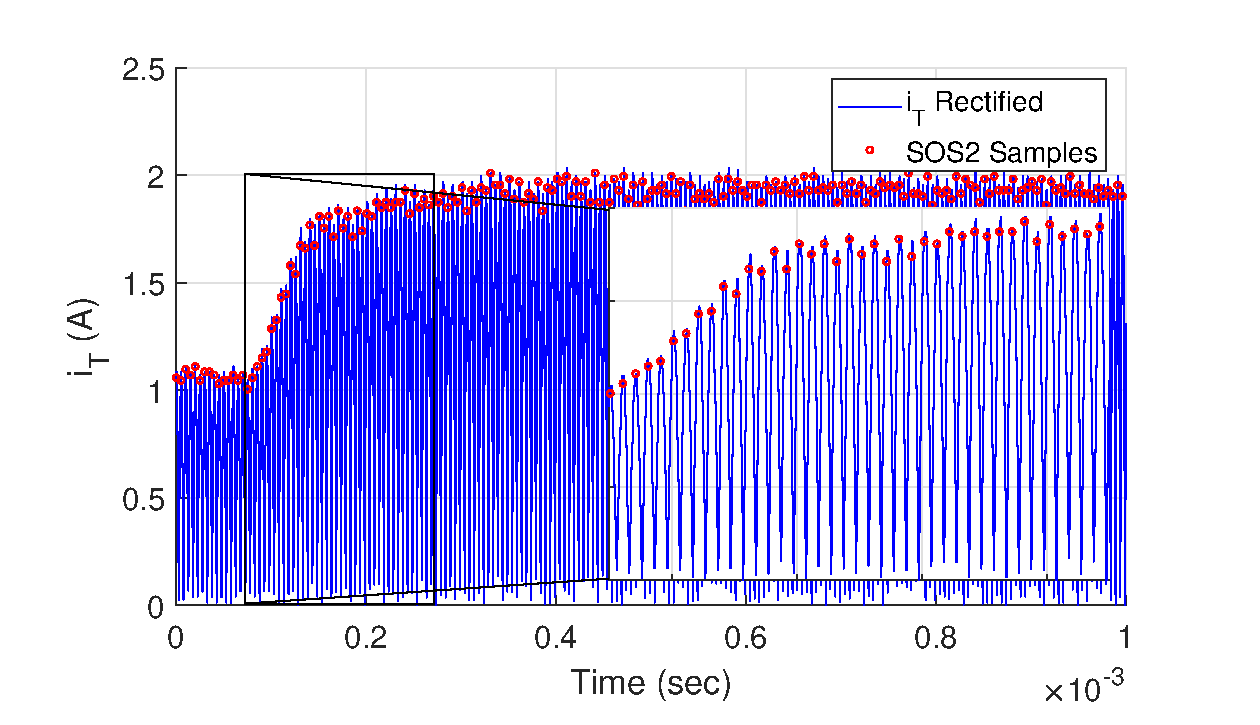
\includegraphics[clip, trim=0mm 1mm 0mm 6mm, width=1\columnwidth]{FIGS/FIG20A.eps}
	                }
	                \\
	                \vspace{-3mm}
	        \subfloat[]{
	                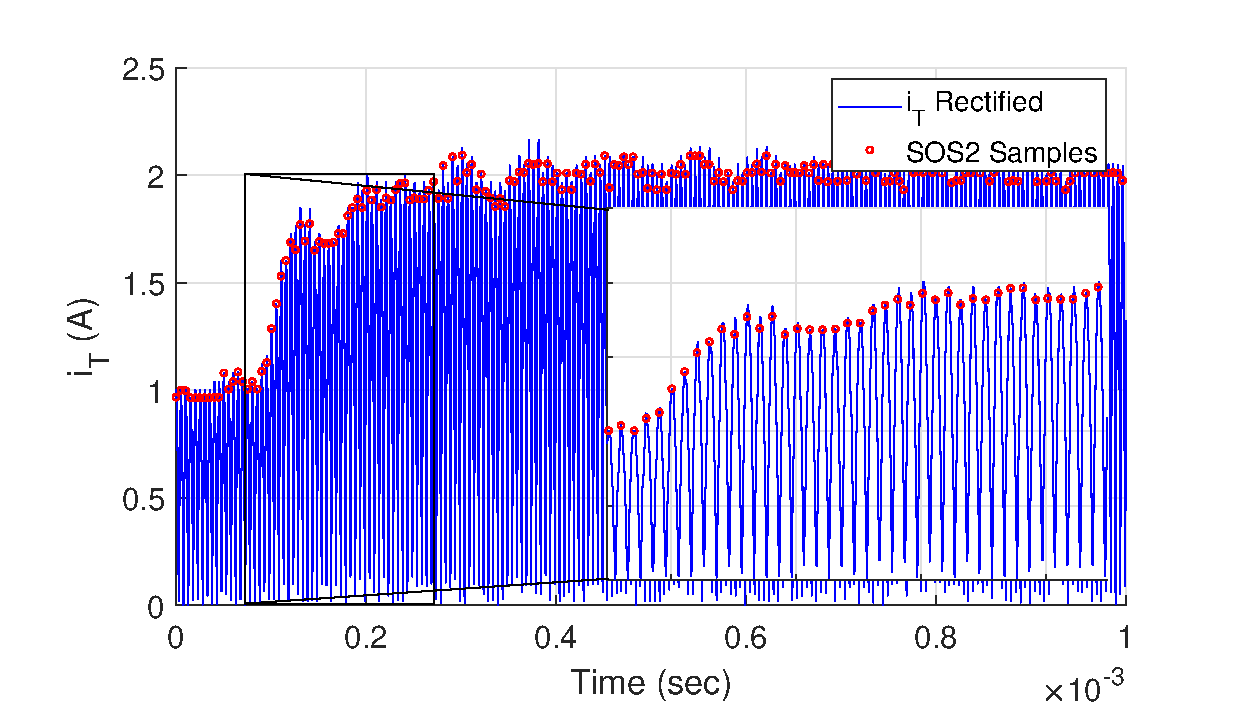
\includegraphics[clip, trim=0mm 1mm 0mm 6mm, width=1\columnwidth]{FIGS/FIG20B.eps}
	                }
	    \end{center}
	    \vspace{-3mm}
	    \caption{Experimental results for a 50\% change in the step change of input voltage for (a) no-load condition (no coupling between transmitter and receiver) and (b) loaded condition (transmitter and receiver interact).}
	    \label{FIG22}
	    \vspace{-3mm}
	\end{figure}
	
	\section{Conclusion}
	Deriving the dominant behavior of an LCC wireless power transmitter pad in its effective range of operation, a new technique of envelope estimation is proposed in this article. Owing to the simplicity of synchronization with PWM signals and minimum required rate of sampling, the proposed technique offers a simple solution to observe and control the dynamic behavior of high frequency systems. 
	%This technique can effectively estimate the envelope of the output signal, and
	%The angle of sampling is tuned accordance to the dominant behavior of the envelope transfer function, and the controller is tuned to apply a proper bandwidth to stabilize the system with a minimum rate of sampling.
	%{\color{blue}It is shown that the envelope transfer function is obtainable by making a vertical shift in its $s$-parameter at the size of the input signal fundamental frequency $\omega_0$.} Therefore, by properly tuning the controller, an effective bandwidth of frequency is applied to the plant (the proposed wireless power transfer system).
	%By taking at least one sample in each cycle of fundamental (in the effective frequency bandwidth of operation), it can evaluate the envelope of the output signal $i_\mathrm{T}$, and it can be effectively used to stabilize the system dynamics. 
	By using the proposed technique of sampling, the quadrature component of $i_\mathrm{T}$ can be obtained, and it can lead to the determination of its envelope effectively so that the system can be stabilized.
	With the use of Nyquist stability analysis, the effectiveness of this sampling technique for a simple PI control loop is studied. To have a more realistic view of this concept, the system under study is simulated and experimentally tested, and the obtained results prove the validity of the proposed sampling technique.
	
	%\appendix[Proof of the Zonklar Equations]
	\vspace{0cm}
	\appendix
	%% APPENDIX A
	%\section
		 \begingroup
	 \footnotesize
	  %%EQ12
	  \sloppy{
	\begin{flalign}
	    \mathfrak{H}_\mathrm{R}(s)=&&
	    \nonumber
	\end{flalign}
	\begin{flalign}
	    \mathrm{G}
	    \frac{\left(s-\sigma\right){\left(\omega_1+\omega_2-2\omega_0\right)}}{(s^2-2\sigma s+(\omega_1-\omega_0)^2-\sigma^2)(s^2-2\sigma s+(\omega_2-\omega_0)^2-\sigma^2)}&&
	    \label{EQ12}
	\end{flalign}
	}
	%%EQ13
	\begin{flalign}
	    \mathfrak{H}_\mathrm{I}(s)=&&
	    \nonumber
	\end{flalign}
	\begin{flalign}
	    -\mathrm{j}\mathrm{G}
	    \frac{\left(s^2-2\sigma s+\sigma^2-(\omega_1-\omega_0)(\omega_2-\omega_0)\right){\left(\omega_1+\omega_2-2\omega_0\right)}}{(s^2-2\sigma s+(\omega_1-\omega_0)^2-\sigma^2)(s^2-2\sigma s+(\omega_2-\omega_0)^2-\sigma^2)}&&
	    \label{EQ13}
	\end{flalign}
	\endgroup
	 
	 
	 \noindent where,
	 
	 \begingroup
	 \footnotesize
	 \begin{flalign}
	 \mathrm{G}=\frac{\omega_0}{C_{\mathrm{P}}L_{\mathrm{S}}L_{\mathrm{TT}}\left(\omega_0+\omega_1\right)*\left({\omega_0+\omega_2}\right)}&&
	 \nonumber
	 \end{flalign}

     \begin{flalign}
	 \sigma=
	 \underbrace{
	 \left(
	 \frac{1}{3}
	 \right)
	 }_{\text{Refining Coefficient}}
	 \frac{(1+\sqrt{3})}{4}
	 \left(
	 \frac{1}{Q_{\mathrm{S}}}+\frac{1}{Q_{\mathrm{T}}}
	 \right)
	 \omega_0&&
	 \nonumber
	 \end{flalign}

	 \begin{flalign}
	 \omega_1=
	 \left(
	 \sqrt{1+(1-K_\mathrm{SSF})\frac{L_\mathrm{S}}{L_\mathrm{TT}}
	 \left(
	 \frac{1}{2}+
	 \sqrt{\frac{1}{4}+(1-K_\mathrm{SSF})^{-2}\left(\frac{L_\mathrm{S}}{L_{\mathrm{TT}}}\right)^{-1}}
	 \right)
	 }
	 \right)\omega_0&&
	 \nonumber
	 \end{flalign}
	 
	 \begin{flalign}
	 \omega_2=
	 \left(
	 \sqrt{1+(1-K_\mathrm{SSF})\frac{L_\mathrm{S}}{L_\mathrm{TT}}
	 \left(
	 \frac{1}{2}-
	 \sqrt{\frac{1}{4}+(1-K_\mathrm{SSF})^{-2}\left(\frac{L_\mathrm{S}}{L_{\mathrm{TT}}}\right)^{-1}}
	 \right)
	 }
	 \right)\omega_0&&
	 \nonumber
	 \end{flalign}
	 
	 \endgroup
	 
	\bibliographystyle{IEEEtran}% bib style
	\bibliography{bibliography}
	\vspace{-1cm}
	% BIOGRAPHIES START HERE	
	\begin{IEEEbiography}[{
\includegraphics[width=1in,height=1.25in,clip,keepaspectratio]{FIGS/Farzad.jpg}}]
	{Farzad Farajizadeh} 
	(Farajizadeh) (S’14-M'20) received the B.Sc. degree in electrical engineering from the Azad University of Gonabad, Iran, in 2009, the M.S. degree in electrical engineering from the Azad University of Tehran, Tehran, Iran, in 2010, and the Ph.D. in electrical engineering from Queensland University of Technology, Brisbane, Australia, in 2021. He is currently doing his research on wireless power transfer systems, power electronic converters, machine drives, renewable energy conversion, and FACTs.
	\end{IEEEbiography}
    
    \vspace{-1cm}
	\begin{IEEEbiography}
	[{
\includegraphics[width=1in,height=1.25in,clip,keepaspectratio]{FIGS/Mahinda.jpg}}]
	{D. Mahinda Vilathgamuwa}
	(S’90–M’93– SM’99) received the B.Sc. degree in electrical engineering from the University of Moratuwa, Sri Lanka, in 1985, and the Ph.D. degree in electrical engineering from Cambridge University, U.K., in 1993. He joined the School of Electrical and Electronic Engineering, Nanyang Technological University, Singapore, in 1993. He is currently a Professor of power engineering with the Queensland University of Technology, Brisbane, QLD, Australia. He has published over 300 research papers in refereed journals and conferences. His research interests include wireless power, power electronic converters, battery storage, and electromobility. He is an associate editor of IEEE Transactions on Industrial Electronics.
	\end{IEEEbiography}
	
	\vspace{-1cm}
	\begin{IEEEbiography}
	[{
\includegraphics[width=1in,height=1.25in,clip,keepaspectratio]{FIGS/Dejan.png}}]
	{Dejan P. Jovanovic }
	(M'05) received the B.Sc. (Dipl. Ing.) degree in electrical and microelectronic engineering and the M.Sc. degree in systems control engineering from the University of Belgrade, Belgrade, Serbia, in 1996 and 2002, respectively, and the Ph.D. degree in statistics from the University of Queensland, Brisbane, QLD, Australia, in 2014. He has held different positions both in industry and academia. He is currently with the Queensland University of Technology, Brisbane, as Research Fellow within the power engineering group. His research interests include control systems, power electronics and application of machine learning in fault diagnosis and fault-tolerant control. Dr. Jovanovic won the IEEE 2005 Future Energy Challenge for a single-phase adjustable speed motor drive.
	\end{IEEEbiography}
	
	
	\begin{IEEEbiography}
	[{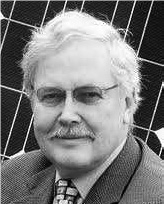
\includegraphics[width=1in,height=1.25in,clip,keepaspectratio]{FIGS/Gerard.png}}]
	{Gerard Ledwich}
	(SM’89) received the Ph.D. degree in electrical engineering from the University of New-castle, Newcastle, NSW, Australia, in 1976. He is a research Professor of electric power with the School of Electrical Engineering and Computer Science, Queensland University of Technology, Brisbane, QLD, Australia. His research interests include power systems, power electronics, and wide area control of smart grid.
	\end{IEEEbiography}
	%% BIOGRAPHIES END HERE
	\vspace{5cm}
	
\end{document}